
\documentclass[master]{thesis-uestc}
\usepackage{listings}  % 引入 listings 宏包,用于显示代码
\usepackage{enumitem}
\usepackage{placeins}  % 导言区添加
\usepackage{tabularx}
\usepackage{array} % 若未加载 array 宏包
\usepackage{makecell}
\usepackage{xeCJK}
\usepackage{fontspec}
\title{面向长尾分布的对比学习故障诊断方法研究}{}

\author{王本浩}{Wang Benhao}
\advisor{周雪\chinesespace 教授}{Dr. Xue Zhou}
\school{电子科技大学(深圳)高等研究院}{Shenzhen Institute for Advanced Study, UESTC}
\major{电子信息}{Electronic Information}
\studentnumber{202222280517}
% \author{王本浩}{Wang Benhao}
% \advisor{*\chinesespace *}{*}
% \school{电子科技大学(深圳)高等研究院}{Shenzhen Institute for Advanced Study, UESTC}
% \major{电子信息}{Electronic Information}
% \studentnumber{202222280517}
% \author{*}{*}
% \advisor{*\chinesespace 教授}{*}
% \school{电子科技大学(深圳)高等研究院}{Shenzhen Institute for Advanced Study, UESTC}
% \major{电子信息}{Electronic Information}
% \studentnumber{*}
\begin{document}

\makecover

\begin{chineseabstract}
    随着工业系统复杂度的不断提升,设备智能监测与故障诊断技术在保障工业生产安全和高效运行中扮演着关键角色。现实工业环境中的故障检测数据通常呈现典型的长尾分布,即头部类别(如正常状态)样本数量充足,而尾部类别(如罕见故障)样本稀少,造成严重的数据不平衡问题。这种长尾分布导致传统诊断模型往往偏向于头部类别,降低了对尾部故障的识别能力,影响了整体诊断效果和泛化能力。自监督对比学习作为一种无需大量标签即可学习有效特征的技术,近年来在故障诊断领域获得广泛关注。然而,现有对比学习方法一定程度依赖人工设计的数据增强模块,其性能受增强策略的差异性和语义一致性显著影响,在故障特征微弱或数据复杂的场景下表现出较大波动,且缺乏自适应调整能力,限制了其在工业实际中的应用。

    为此,本文提出了一种基于自适应数据增强优化的对比学习故障诊断框架。该框架通过对比学习训练编码器,并对编码器提取的特征质量进行动态评估,利用 CMA-ES 算法作为控制器,自动调整数据增强模块的参数。以线性评估准确率作为反馈指标,解决了传统人工设计增强方法在准确性与多样性上的不足,有效促进孪生网络学习到更深层次的语义特征。在 CWRU 数据集上,本文方法在 SimSiam、SimCLR、BYOL、SwAV 和 MoCo v2 等五种主流对比学习模型上均取得显著提升。在训练集样本均匀分布时,在两个数据集上平均提升达2.56\%。在样本不平衡度极高的条件下,在两个数据集上平均提升达3.92\%,充分展示了其对长尾分布数据的鲁棒性和适应性。

    进一步地,本文设计了结合半监督学习与基于类别边距调节优化了微调过程的两阶段微调方法(Semi-Marc),该方法在微调阶段引入决策边界动态调整机制,有效缓解了长尾分布对分类层性能的负面影响。通过伪标签指导的半监督训练和边界优化,Semi-Marc 显著提升了模型对尾部故障类别的识别能力。实验结果表明,在自适应数据增强优化基础上,Semi-Marc 方法在多种主流对比学习模型中均实现进一步性能提升,在两个数据集上平均提升约1.78\%,验证了其良好的通用性和有效性。综上所述,本文提出的方法为解决长尾分布下的故障诊断问题提供了有力支持,具有较好的应用前景和推广价值。


\chinesekeyword{故障诊断,长尾学习,对比学习,孪生网络}
\end{chineseabstract}

\begin{englishabstract}
    With the increasing complexity of industrial systems, intelligent monitoring and fault diagnosis technologies play a crucial role in ensuring the safety and efficient operation of industrial production. In real-world industrial environments, fault detection data often exhibits a typical long-tailed distribution: head classes (e.g., normal condition) have sufficient samples, while tail classes (e.g., rare faults) have very few, leading to a severe data imbalance problem. This long-tailed distribution causes traditional diagnostic models to be biased toward head classes, thereby reducing their ability to identify tail faults and affecting the overall diagnostic performance and generalization capability. Self-supervised contrastive learning, as a technique that can learn effective features without requiring large amounts of labeled data, has received widespread attention in the fault diagnosis field in recent years. However, existing contrastive learning methods still partially rely on manually designed data augmentation modules, and their performance is significantly affected by the variability and semantic consistency of the augmentation strategy. In scenarios where fault features are weak or data is complex, these methods show large performance fluctuations and lack adaptive adjustment capabilities, which limit their practical application in industry.

    To address this issue, this thesis proposes a contrastive learning fault diagnosis framework optimized by adaptive data augmentation. This framework trains an encoder via contrastive learning and dynamically evaluates the quality of features extracted by the encoder. The CMA-ES algorithm is used as a controller to automatically adjust the parameters of the data augmentation module. By using linear evaluation accuracy as a feedback indicator, the proposed method solves the limitations of traditional manually designed augmentation in terms of accuracy and diversity, and effectively promotes the learning of deeper semantic features by the twin networks. On the CWRU dataset, the proposed method shows significant improvements across five mainstream contrastive learning models, including SimSiam, SimCLR, BYOL, SwAV, and MoCo v2. When the training samples are uniformly distributed, the average improvement on two datasets reaches 2.56\%. Under conditions of extremely high data imbalance, the average improvement reaches 3.92\%, fully demonstrating its robustness and adaptability to long-tailed data.

    Furthermore, this thesis designs a two-stage fine-tuning method, Semi-Marc, which combines semi-supervised learning and category-margin-based adjustment to optimize the fine-tuning process. This method introduces a dynamic decision boundary adjustment mechanism during fine-tuning, effectively mitigating the negative impact of long-tailed distribution on the classification layer. Through semi-supervised training guided by pseudo-labels and boundary optimization, Semi-Marc significantly enhances the model's ability to identify tail fault classes. Experimental results show that, based on adaptive data augmentation optimization, the Semi-Marc method achieves further performance improvements across multiple mainstream contrastive learning models, with an average improvement of approximately 1.78\% on two datasets. This verifies its good generalization and effectiveness. In summary, the method proposed in this thesis provides strong support for solving fault diagnosis problems under long-tailed distribution and demonstrates promising application potential and practical value.


\englishkeyword{Fault Diagnosis, Long-Tail Learning, Contrastive Learning, Siamese Network}
\end{englishabstract}

\thesistableofcontents

\chapter{绪\hspace{6pt}论}

\section{研究工作的背景与意义}

智能故障诊断是预测性健康管理(Prognostics and Health Management, PHM)系统中的核心组成部分,旨在实现设备故障的高效检测与精准识别,从而保障系统的安全与稳定运行。PHM 技术在各类关键工业装备中得到广泛应用,如复杂机械系统和高精度运转设备,具有重要的工程实践价值。智能故障诊断的有效性直接关系到生产过程的安全性、连续性与可靠性,具有重要的现实意义。例如,旋转机械是现代工业中的核心设备,长期在高温、疲劳、重载等复杂工况下运行,若发生故障,不仅可能引发严重事故,还会造成巨大的经济损失,甚至威胁人员安全。

智能故障诊断技术已在多个典型工业领域得到广泛应用,包括制造业与工业自动化领域,通过对生产设备的状态监测和故障预警,有效提升生产效率和设备利用率;轨道交通与桥梁监测领域,利用故障诊断技术保障交通运输安全及基础设施的长期稳定;以及医疗设备领域,智能诊断有助于确保医疗设备的可靠性与医疗服务的连续性。

\begin{figure}[h!]
    \centering
    \subfloat[]{
        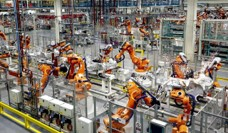
\includegraphics[width=0.3\textwidth]{app1.jpg}
        \label{fig:app1}
    }
    \subfloat[]{
        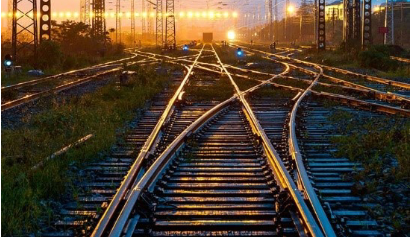
\includegraphics[width=0.3\textwidth]{app2.png}
        \label{fig:app2}
    }
    \subfloat[]{
        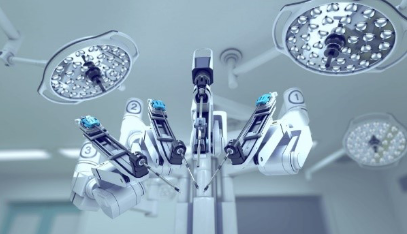
\includegraphics[width=0.3\textwidth]{app3.png}
        \label{fig:app3}
    }
    \caption{智能故障诊断的典型应用场景示意图:(a) 制造业与工业自动化;(b) 轨道交通与桥梁监测;(c) 医疗设备}
    \label{fig:application_scenes}
\end{figure}

在高维特征空间中,许多人工构造的特征可能存在冗余性或与目标任务无关,进而导致分类器性能波动,甚至引发过拟合问题,影响模型的泛化能力。特征提取的难题不仅增加了诊断系统的复杂性和实施成本,还影响了故障诊断模型的稳定性、可靠性和适用性。因此,如何自动化、智能化地提取具有鲁棒性和泛化能力的故障特征,成为智能故障诊断领域亟待解决的重要问题。

现实中的故障检测数据通常呈现长尾分布,这是一种偏态分布,其中头部类包含大量正常数据,而尾部类则包含较少的故障数据。长尾分布数据在现实世界中广泛存在,大规模数据集通常呈现出长尾分布的特性。面向长尾分布数据的学习任务,是故障诊断领域普遍面临的挑战之一,尤其在稀有故障的识别中更为突出。例如,正常工作状态的数据通常远多于故障工作状态,或者常见故障状态的数据量远多于罕见故障状态。现实中的故障检测数据往往服从长尾分布,这种分布是一种典型的偏态分布,如图~\ref{fig_long_tail}所示:大规模训练数据中,头部类别的样本数量占据主导地位,而尾部类别的样本数量相对稀少,并呈现逐渐递减的趋势。长尾分布的数据常伴随显著的样本不平衡问题,导致训练过程中模型倾向于关注头部类别,从而削弱了对尾部类别的识别性能。当样本分布均衡时,各类别在特征空间中具有清晰的区分边界,并占据较宽广的特征空间。然而,当数据分布失衡呈现长尾分布时,尾部类别的特征分布变得狭窄,并依附于头部类别附近,从而扭曲了特征空间结构,降低了类别间的多样性与区分性。在使用长尾数据训练神经网络时,模型性能容易受到头部类别的影响,导致尾部类别的表现较差。然而,对尾部类别样本的错分往往带来更大的实际损失,因此研究尾部类别样本具有重要的现实意义。如何基于长尾分布的故障检测数据有效训练故障检测模型,已成为一个具有重要价值的研究难题。
\begin{figure}[h]
    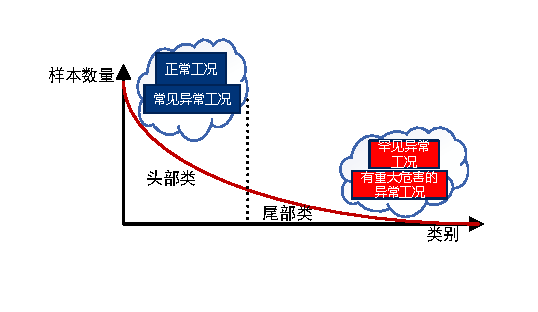
\includegraphics[width=9cm]{long_tail.pdf}
    \caption{长尾分布示意图}
    \label{fig_long_tail}
\end{figure}

长尾分布数据对现代深度学习框架提出了巨大的挑战。即使使用数据重采样、类平衡损失等专门技术,在极端类不平衡的情况下,模型性能仍然显著下降。因此,为了更有效地应对这一挑战,深入理解长尾学习对特征分布的影响至关重要。然而,与平衡数据的学习情景不同,长尾学习中的标签扮演着一个复杂而矛盾的角色,形成了标签价值的困境。一方面,有标签的监督学习通常比无监督学习能够训练出更准确的分类器,这突显了标签的积极作用;另一方面,长尾的标签分布会自然引入“标签偏差”,其中头部类别在很大程度上驱动决策边界的学习,导致对尾部类别的压制。这表明,标签既是推动学习的动力,也可能成为性能下降的原因,可以说是一把双刃剑。自监督学习的提出旨在减少对人工标注数据的依赖,使得即便在缺乏标注数据的情况下,网络仍能高效地进行训练。自监督学习在预训练阶段通过人工构造输入数据的代理任务使特征层网络学习到有效的特征表示,完全摆脱了对标签的依赖。只在对最终的分类器层进行微调过程中运用了标签,从而最大限度地减小“标签偏差”带来的影响。文献\cite{zhang2021federated}指出,额外的自监督预训练能够显著提升常规长尾学习算法的性能,并已在CIFAR-LT、ImageNet-LT等视觉识别长尾数据集上得到验证。尽管在故障诊断的长尾学习领域,半监督学习、集成学习、样本加权等方法已经取得一定进展,但应用自监督学习方法的研究仍相对较少。因此,应用自监督学习解决长尾分布数据故障诊断问题仍是一个具有重要意义的研究方向。
% \begin{figure}[h]
%     \subfloat[]{
%         \label{tsne_mean_distribution}
%         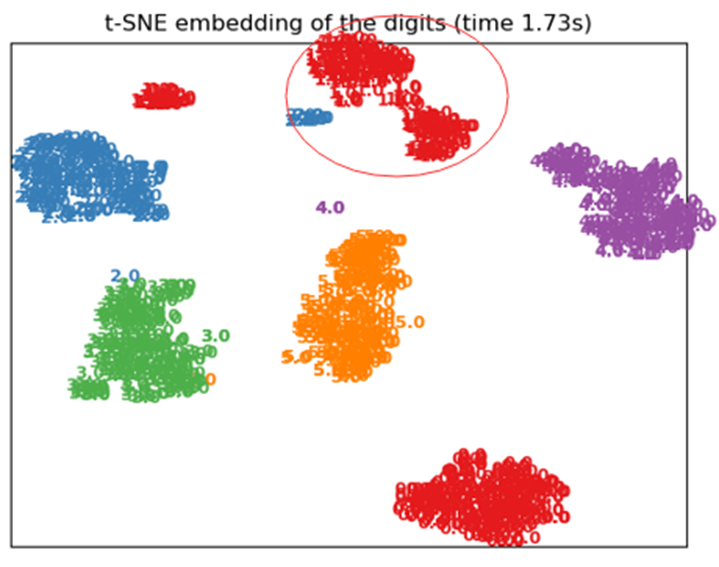
\includegraphics[width=6.77cm]{tsne_mean_distribution.png}
%     }
%     \subfloat[]{
%         \label{tsne_lt_distribution}
%         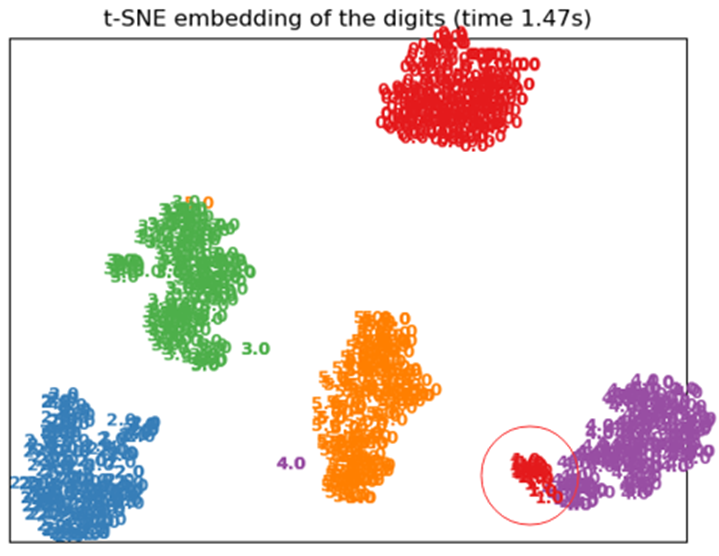
\includegraphics[width=6.77cm]{tsne_lt_distribution.png}
%     }
%     \caption{均匀/长尾分布数据的tsne图(a)样本均匀分布时的T-SNE分布图(b)尾部类“1”类样本个为30,头部类样本个数为180个时的T-SNE分布图}
%     \label{long-tail result}
% \end{figure}

% 目前,在视觉识别领域,长尾学习已提出多种前沿方法,如变分自编码器\citing{kingma2013auto}、生成对抗网络\citing{goodfellow2020generative}、CB(Class-Balanced)Loss\citing{cui2019class}、自监督学习\citing{yang2020rethinking}、以及Marc决策面调整算法\citing{wang2023margin}等。然而,在故障诊断的长尾学习领域,常见的方案包括半监督学习\citing{nanjing2023faultdetection}、集成学习\citing{吴亮2023基于多级学习的长尾分布下交通多目标检测}、样本加权\citing{cumm2023faultdiagnosis}等,相较而言,前沿的长尾学习方法在故障诊断中的应用较少。因此,提出一个结合前沿长尾学习方法的故障诊断模型具有重要的现实意义。
\FloatBarrier  % 阻止后续浮动体越过这条线

\section{故障诊断基本流程}
故障诊断的基本流程通常包括数据采集、信号预处理、特征选择、模型训练与优化、以及故障识别与诊断结果分析等步骤。在现代工业系统中,设备状态的监测依赖于多种传感器,如加速度传感器、声发射传感器、电流传感器和温度传感器等,以采集振动、声音、电流和温度等信号,从而提供反映设备健康状况的数据基础。由于采集到的原始信号往往受到噪声干扰,信号预处理成为数据分析的关键步骤,常见的方法包括滤波、归一化、去趋势以及信号分解,以提高数据质量并增强关键特征的可识别性。

在信号预处理的基础上,特征提取是故障诊断中的核心环节,其目的是从原始信号中提取能够反映设备运行状态的关键信息。根据信号分析方式的不同,特征可以分为时域、频域和时频域特征。时域特征如均值、均方根、偏度、峰值因子和峭度等,主要用于描述信号的统计特性;频域特征通过傅里叶变换提取主频分量、功率谱密度和边频带特征,以揭示设备的动态特性;时频域特征则通过小波变换、短时傅里叶变换或其他时频分析方法提取,分析信号的非平稳性和时变特征。由于部分手工提取的特征可能存在冗余或无关信息,特征选择成为优化故障诊断性能的重要手段,通常采用主成分分析、互信息分析或递归特征消除等方法筛选最具诊断价值的特征,本文构造了深度神经网络并采用自监督学习方法训练特征层网络提取深层特征。

在获得高质量的特征后,模型训练是智能故障诊断系统构建的核心环节。传统的机器学习方法,常见的分类方法包括支持向量机、随机森林、K近邻和决策树等,依赖于人工构建的特征,能够在特定工况下实现较高的分类精度。然而,随着深度学习的发展,卷积神经网络、循环神经网络、Transformer和图神经网络等深度学习模型展现出更强的特征自动提取和故障识别能力,特别是在面对复杂工况和海量数据时,其优势尤为明显。由于工业环境中的数据分布通常存在不均衡问题,模型训练过程中需要考虑数据重采样、类别平衡损失等策略,以降低类别不平衡对故障识别能力的影响。此外,超参数优化在提升模型泛化能力和稳定性方面也起着至关重要的作用。

在训练得到故障诊断模型后,测试数据的输入可实现自动故障识别与分类。常见的故障类型包括轴承故障(如滚动体故障、内圈故障和外圈故障)、齿轮故障(如齿面点蚀、断齿和偏磨)以及电机故障(如定子故障、转子故障)等。故障分类的准确性通常采用准确率、召回率、F1-score等指标进行评估,以确保模型的可靠性和实用性。最终,故障诊断的核心目标是为设备维护和运行决策提供有效支持。通过诊断结果分析,可以实现设备健康状态评估、故障预警、剩余寿命预测以及故障溯源分析等功能,从而优化维护策略,提高设备运行的安全性和可靠性。随着深度学习、迁移学习和自监督学习等技术的不断发展,智能故障诊断方法正在逐步突破传统方法的局限,未来研究将进一步探索如何在复杂工况下提升诊断模型的鲁棒性和适用性,以推动智能运维的发展。
\FloatBarrier  % 阻止后续浮动体越过这条线

\section{故障诊断的研究现状}
近年来,故障诊断的研究如火如荼。薛阳等人\citing{xue2022multimodal}基于CWRU滚动轴承故障数据提出将多模态结合与卷积神经网络相结合,提取时域和频域两个模态的特征,实现时频域双模态结合对故障类型的联合诊断,相较于单时域或单频域的卷积神经网络故障诊断模型均有提升。郭文军等人\citing{郭文军2022EMD}构建了经验模态分解与自回归相结合的深度特征提取方法,增强了隐层筛选故障特征的能力。特征提取在构建故障诊断模型中至关重要,因此得到了国内外学者的广泛关注。传统时域信号特征提取方法,如快速傅里叶变换、小波包分解、小波变换和经验模态分解均有良好应用。近年来,随着神经网络的发展,基于机器学习的特征提取方法也迅速发展,诸如基于粒子群优化的自适应多稳态欠阻尼随机共振方法\citing{杨波2022自适应随机共振在信号特征提取中的应用},堆叠自动编码器\citing{蒋爱国2018基于多模态堆叠自动编码器的感应电机故障诊断},多尺度核卷积神经网络\citing{李永刚2023一种基于},以及利用递归图编码将振动信号转换为增强信号特征的二维图像的技术\citing{张龙2023采用递归图编码技术与残差网络的滚动轴承故障诊断}均取得了显著成果。

随着深度学习技术的快速发展,故障诊断领域涌现出大量基于深度神经网络的方法,进一步提升了故障识别的准确率和自动化程度。卷积神经网络因其强大的特征提取能力,广泛应用于时域、频域及时频域信号的特征学习。周文宣等人\citing{周文宣2021一种基于多尺度卷积神经网络的滚动轴承故障诊断方法}基于多尺度卷积神经网络实现了旋转机械故障识别,显著提升了复杂工况下故障检测效果。循环神经网络与长短时记忆网络在序列数据建模方面表现出色,适用于机械振动等时间序列信号的故障诊断。

与此同时,自监督学习与对比学习技术逐渐受到关注。通过设计预训练任务,无需大量标注数据即可学习具有判别力的特征表示。孙伟等人提出基于对比学习的轴承故障诊断方法,有效提升了模型对未知故障类型的识别能力。孪生网络作为对比学习的重要架构,通过构建正负样本对优化相似度度量,在故障诊断领域得到应用,有效缓解了标签稀缺问题。

然而,实际工业数据中普遍存在长尾分布现象,大多数故障类型样本稀少,少数类别样本丰富,严重影响诊断模型的泛化能力和尾部类别识别准确率。针对这一问题,部分研究开始采用长尾学习策略,包括重采样、重加权以及基于边距调整的决策边界校准,提升尾部类别的检测性能。尽管如此,结合自监督学习和长尾学习的研究仍较有限,且如何充分利用无标签数据辅助模型学习仍是关键挑战。

综上,智能故障诊断领域正经历从传统特征工程向端到端深度学习与自监督学习的转变,长尾分布和样本不平衡成为研究重点。本文基于对比学习与自监督学习框架,结合自适应数据增强和半监督边距调整技术,致力于提升故障诊断模型在长尾场景下的鲁棒性和识别性能。


\section{长尾分布下的自监督与对比学习研究现状}
\subsection{长尾学习研究现状}
在现实世界中,许多任务的数据分布存在“长尾”现象,即少数类样本数量远少于多数类样本,导致模型在训练时更倾向于学习头部类(多数类)的特征,而忽视尾部类(少数类)。这种类别不平衡现象在故障诊断任务中尤为常见,特别是在设备健康状态数据采集中,正常状态样本往往远多于各类故障状态,容易造成诊断模型对少见故障识别能力不足。

针对这一问题,国内外学者提出了多种应对策略,主要分为三个方面,如图~\ref{longtail_solution}所示:

首先是在样本层面进行调整,包括欠采样与过采样。欠采样方法如随机欠采样、NearMiss~\citing{shen2016near}、编辑最近邻(ENN)~\citing{wilson1972asymptotic}等,试图通过减少头部类样本平衡整体数据分布;过采样方法如随机过采样、SMOTE~\citing{chawla2002smote}、变分自编码器(VAE)~\citing{kingma2013auto}和生成对抗网络(GAN)~\citing{goodfellow2020generative}等则致力于通过合成新样本扩充尾部类数量。然而,采样策略可能引入噪声,影响数据分布的真实性,导致模型误判或过拟合。

其次是在损失函数层面引入类别平衡机制,通过修改损失函数的权重以强调尾部类样本。例如,类频率逆加权方法~\citing{huang2016learning},在线难例挖掘(OHEM)与Focal Loss~\citing{lin2017focal}通过对难分类样本赋予更高权重,增强模型对不平衡数据的敏感性。Cui等人提出的CB(Class-Balanced)Loss~\citing{cui2019class}通过引入与“有效样本数”相关的平衡因子,进一步缓解了极度不均的类别分布。

第三类方法是模型结构层面的改进,包括集成学习、自监督学习、迁移学习、度量学习与元学习等新兴技术。例如,Marc(Margin Calibration)算法~\citing{wang2023margin}通过边距调整优化模型的决策边界,有效提升尾部类识别能力。Yang等人~\citing{yang2020rethinking}结合半监督与自监督学习,在无标签数据中进行伪标签扩充,改善尾部类特征分布,提高整体模型性能。此外,通过结构解耦,即在特征提取器与分类器之间建立独立训练机制~\citing{zhou2020bbn,kang2019decoupling},可缓解分类器对头部类的依赖性,从而增强尾部类识别能力。

目前,国内外对长尾学习问题的研究已取得丰富成果。例如,Liu等人~\citing{liu2020deep}提出一种基于“特征云”的数据增强方法,利用头部类样本的类内方差信息迁移至尾部类,以提升尾部类特征表达能力,该方法已在面部识别中验证有效性。Yang等人~\citing{yang2020rethinking}通过自监督预训练和半监督微调相结合的方法显著提高长尾分类准确性,并指出高维特征空间中的对比学习在长尾学习中具有明显优势。

在图像识别领域,吴磊等人~\citing{wu2023personalized}设计了结合残差结构的多专家识别框架,通过个性化信息增强模块和两阶段训练机制,有效提高中尾部类别的识别性能。吴亮等人~\citing{吴亮2023基于多级学习的长尾分布下交通多目标检测}则提出多级分组分类器与注意力特征重结合模块,通过Logit联合调整缓解组间不平衡问题,实现了更高的精度与鲁棒性。

\begin{figure}[h]
    \centering
    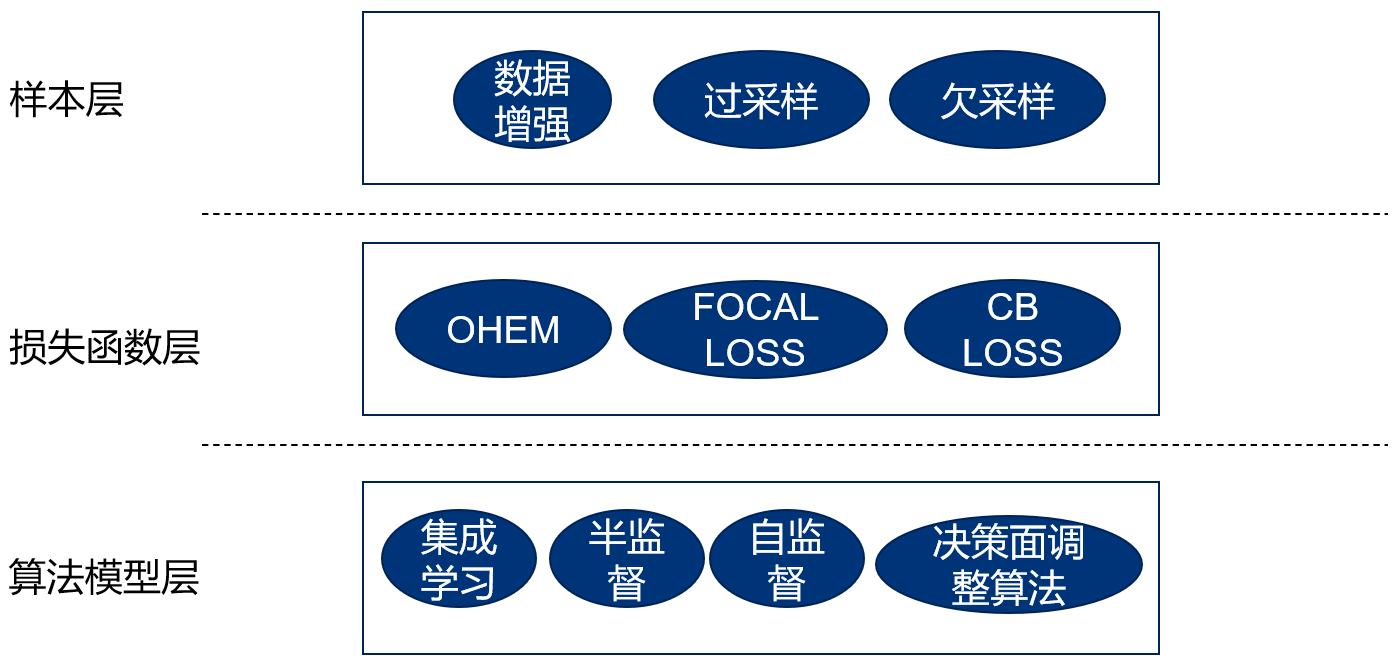
\includegraphics[width=11cm]{longtail_solution.png}
    \caption{长尾学习常见方法}
    \label{longtail_solution}
\end{figure}

综合来看,目前多数研究集中在计算机视觉领域,尤其是在CIFAR-LT、ImageNet-LT等标准图像数据集上验证算法性能,而在故障诊断这一工业领域,针对长尾学习问题的研究尚不充分。尽管Yang等人~\citing{yang2020rethinking}的研究为故障诊断中应用自监督预训练提供了良好启示,但其对半监督机制的适用性尚待进一步论证。吴磊~\citing{wu2023personalized}与吴亮~\citing{吴亮2023基于多级学习的长尾分布下交通多目标检测}提出的集成学习结构在提升尾部类性能方面表现优异,若结合自监督机制或迁移学习,其性能有望进一步提升。Wang等人~\citing{wang2023margin}提出的Marc算法结构简洁,适应性强,但其在故障诊断中的适用性与有效性仍需深入研究。

因此,将前沿长尾学习方法尤其是自监督对比学习方法引入故障诊断任务中,并在模型的预训练与微调阶段进行系统优化,不仅具有理论创新意义,更具重要的工程应用价值。本文将重点围绕模型层面的改进展开研究,探讨自监督预训练与长尾学习结合的深度诊断框架设计。

\FloatBarrier  % 阻止后续浮动体越过这条线

\subsection{自监督学习的发展历程和研究现状}

2019年,MoCo\citing{He_2020_CVPR}的提出掀起了视觉自监督学习的热潮,随后SimCLR\citing{chen2020simple}、BYOL\citing{grill2020bootstrap}、SwAV\citing{caron2020unsupervised}等主流自监督学习算法相继问世,使得该领域呈现出百花齐放、百家争鸣的繁荣局面。2021年末,MAE\citing{he2022masked}的提出进一步促进了自监督学习的发展,并将其提升到了一个全新的高度。然而,这一成就的背后,自监督学习经历了长期的迭代与发展。

目前,国内外学者对自监督预训练方法展开了大量研究。例如,在计算机视觉领域,Yang等人\citing{yang2020rethinking}研究了不平衡样本标签信息在模型训练中的价值,提出了一种半监督学习方法,该方法通过利用原模型识别无标签数据并生成伪标签来扩充原数据集,并验证了自监督预训练的有效性。此外,该研究还发现,样本维度越高,性能提升越显著,这为自监督预训练在故障诊断长尾学习领域的应用提供了有力支持。Doersch等人\citing{doersch2015unsupervised}提出了基于局部图像块位置预测的自监督任务,随机抽取图像中的两个块,训练模型预测一个块相对于另一个块的位置。Zhang等人\citing{zhang2016colorful}构建了基于图像上色的自监督任务,将图像转换到CIE Lab颜色空间后,提取其中的L通道作为模型输入,引导模型预测对应的a和b通道颜色信息。Gidaris等人\citing{gidaris2018unsupervised}通过人为旋转图像不同角度,并将旋转角度作为监督信号训练模型,从而实现图像语义特征的自监督学习。文献\cite{noroozi2017representation}提出了一种新的表示学习方式,通过基于计数视觉原语的人工监督信号来进行训练,而无需任何人工标注。核心思想是利用图像变换与表示变换之间的等变关系。文献\cite{caron2018deep}提出了利用KMeans算法生成样本的伪标签,将其作为数据的真实标签训练网络,用网络新提取的特征重新生成KMeans伪标签,以此重复。

近年来,自监督预训练方法也逐步应用于故障诊断领域,并受到广泛关注。例如,Zhang等人\citing{zhang2022prior}提出了基于先验知识的自监督任务,利用卷积自编码器进行训练,在小样本学习任务中取得了良好表现。Senanayaka等人\citing{senanayaka2020toward}采用One-Class SVM输出的标签作为代理标签,使用自监督预训练的卷积神经网络进行故障特征提取。W. Zhang等人\citing{zhang2021federated}提出了一种基于信号块交换的自监督任务,即通过打乱时域信号块顺序构造“伪数据”,并训练模型区分原始数据和伪数据。实验结果表明,该方法在特征提取任务中表现优异。

综上所述,尽管文献\cite{doersch2015unsupervised, zhang2016colorful, gidaris2018unsupervised}等研究在计算机视觉领域取得了重要进展,但其方法在故障诊断任务中的直接应用仍面临一定困难。然而,这些研究的思路为故障诊断领域的自监督预训练任务设计提供了有益的启示。例如,文献\cite{senanayaka2020toward}提出的One-Class SVM生成的标签可以结合聚类算法,使其适用于多分类任务;文献\cite{zhang2021federated}提出的信号块交换方法与文献\cite{doersch2015unsupervised}提出的图像块位置预测任务在思路上具有一定相似性,值得探索其结合的可能性。此外,文献\cite{zhang2022prior, senanayaka2020toward, zhang2021federated}提出的自监督预训练方法在任务设计上仍具有较大的创新空间,且在长尾学习任务中的应用尚未得到充分探索。因此,故障诊断领域的自监督预训练仍处于发展初期,借鉴计算机视觉领域的前沿自监督任务,提出更具创新性和更高性能的自监督预训练任务,仍具有重要的研究价值和挑战。
\FloatBarrier  % 阻止后续浮动体越过这条线

\subsection{对比自监督学习和孪生网络的发展历程和研究现状}

自监督学习的核心目标是在无人工标注的情况下自动提取有效特征\citing{min2021cross}。近年来,对比自监督学习作为无监督学习的重要分支之一,通过构造正负样本对,使模型能够学习更具判别性的特征表示。它逐渐成为研究热点,并在图像识别任务中取得了最先进的性能。许多相关算法相继被提出,例如动量对比学习\citing{He_2020_CVPR}、对比预测编码\citing{oord2018representation}以及用于视觉表征学习的简单对比学习框架\citing{chen2020simple}。

这些方法的核心思想是通过拉近相同样本的不同视图(正样本对)并推远不同样本(负样本对)来学习有意义的特征表示。对比学习方法通常依赖存储在记忆库中的大量负样本,以提高对比学习效果\citing{wu2018unsupervised}。此外,一些其他对比学习方法不依赖负样本,而是计算两个正样本对之间的相似性,例如SwAV\citing{caron2020unsupervised}、BYOL\citing{grill2020bootstrap}以及SDCT\citing{yuan2020self}。

在对比自监督学习中,孪生网络(Siamese Network)因其适用于比较不同样本的网络结构,具有独特优势。Laine和Aila\citing{laine2016temporal}提出了基于孪生网络的$\pi$-model,用于训练深度神经网络,该方法在半监督学习场景下依赖不同的正则化规则与数据增强策略。Zheng和Yang\citing{zheng2019unsupervised}提出了一种“记忆正则化”机制,其核心思想是让主模型自身(而非外部模块)学习域内知识,以实现无监督场景自适应。Zhao等人\citing{zhao2021deep}提出了基于相互学习和知识蒸馏的训练方法,以提高视觉目标跟踪任务的性能。SimSiam\citing{chen2021exploring}采用简化的孪生网络结构,该网络无需构造负样本对、大批量训练和动量编码器,并在计算机视觉任务中展现出卓越性能。

由于对比学习模型高度依赖数据增强模块提供的视图差异性与语义一致性,其在故障诊断领域的性能受到增强策略质量的显著影响,尤其在故障特征弱或数据分布复杂的场景下,表现出较大的性能波动。本文从理论上分析了对比学习数据增强模块对训练的意义以及所需要的数据增强方法需要具备的特质,同时通过一种自动搜索最优增强参数的方法解决对比学习需要经过人工挑选数据增强方法和设定数据增强模块的参数的问题。
\FloatBarrier  % 阻止后续浮动体越过这条线

\section{本文的主要贡献与创新}

本论文聚焦于面向长尾分布数据的自监督学习故障诊断,主要的创新点和贡献如下:

\begin{enumerate}[label={(\arabic*)}]
    \item 提出了一种基于自适应数据增强优化的对比学习故障诊断网络框架。该框架引入 CMA-ES 控制策略,根据编码器输出特征的分类性能动态调整数据增强参数,从而提升增强策略的多样性与语义一致性,有效增强模型对复杂和稀疏故障模式的感知能力。
    
    \item 在上述框架基础上,进一步提出并优化了一种结合半监督学习与类别边距调节的两阶段微调方法(Semi-Marc)。该方法通过伪标签引导的半监督学习与决策边界动态调整机制,有效缓解了长尾分布对分类层带来的不利影响,提升了模型对尾部故障类别的判别能力与泛化性能。
\end{enumerate}


\section{本论文的结构安排}

本文的章节结构安排如下:

第一章介绍了研究的背景与意义,分析了传统故障诊断方法在处理长尾分布数据时面临的挑战,并重点回顾了国内外在长尾学习算法领域的研究进展与现有局限性。

第二章阐述了长尾学习与自监督学习范式的基本概念,介绍了为孪生网络对比学习的理论基础,并介绍了实验使用的数据集和研究对象。

第三章提出了基于自适应数据增强优化的对比学习故障诊断网络框架,详细描述了框架各模块的设计与实现,并从实验与理论两个层面验证了框架的有效性。通过准确率、t-SNE分布图以及对无标签数据集规模等参数的敏感性分析,证明了该自适应数据增强框架在现有SOTA的对比学习方法能有较大的提升。

第四章提出了结合半监督边距调整优化的对比学习的微调框架,旨在减轻孪生网络在微调阶段受长尾效应影响的问题。实验结果表明,该微调框架提升了诸多模型的整体性能,展示了其良好的普适性。

第五章总结了全文的研究工作,并对未来可能的研究方向进行了展望。


\chapter{对比学习方法理论与故障诊断数据集基础}
\section{自监督学习相关理论}
自监督学习是一种近年来迅速发展的表示学习范式,旨在无需依赖人工标注的前提下,从大量未标注数据中自动学习出具有泛化能力的特征表示。这一方法的核心在于通过构造合理的辅助任务,生成伪监督信号,进而引导模型在原始数据上进行表征学习。这样一来,模型可以从海量无标签数据中挖掘出潜在的结构规律,学习出能够迁移到下游任务的通用特征。如图~\ref{self_supervise_procedure}所示,自监督学习的整体流程通常可分为两个阶段:首先是预训练阶段,然后是微调阶段。

\begin{figure}[h]
    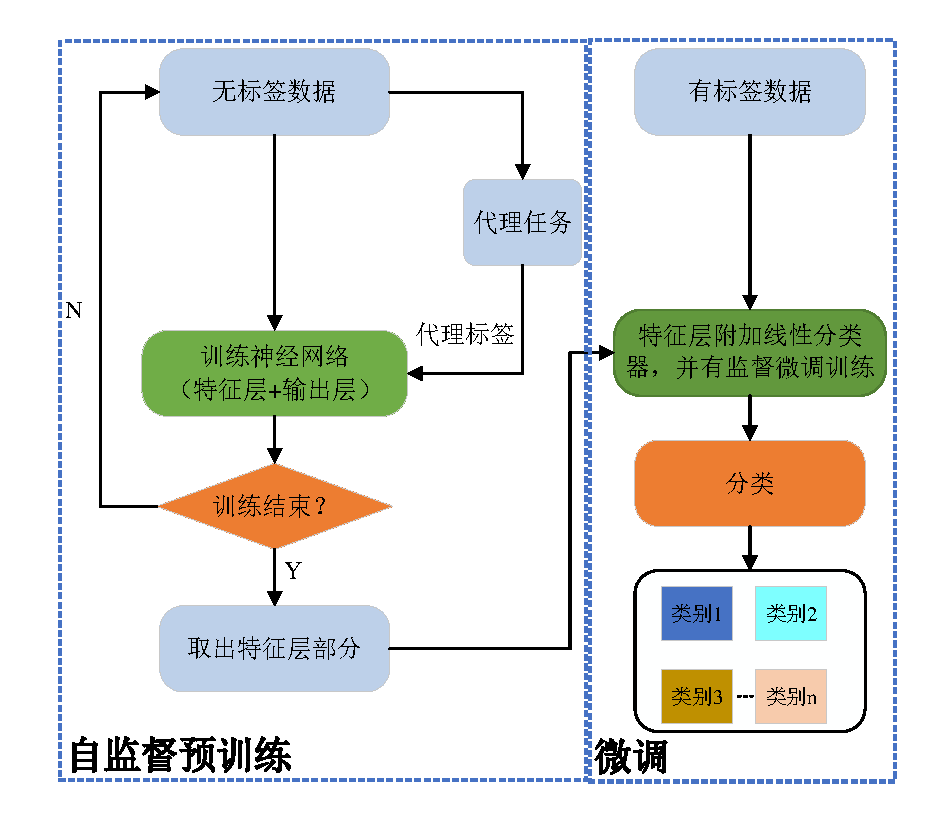
\includegraphics[width=12cm]{self_supervise_procedure.pdf}
    \caption{自监督训练范式流程}
    \label{self_supervise_procedure}
\end{figure}

在预训练阶段,完全不使用人工标注的类别信息,而是依靠数据自身的属性构建任务,引导模型从输入中提取关键特征。常见的辅助任务包括图像重建、遮挡区域预测、视角一致性判断和样本对比等,这些任务都能促使模型学习到更深层次、更具鲁棒性的表征。在这一过程中,模型从数据中获取的信息更加全面,不仅可以规避类别标签稀缺带来的限制,还能有效减缓类别不均衡对模型初始化的影响。由于模型学习到的是数据中的通用结构信息,因此训练出的特征在多种任务和不同数据分布中均具有良好的迁移能力,有助于提升模型的泛化性能。

在微调阶段,利用自监督预训练获得的网络参数作为模型的初始状态,再结合具体任务的监督信号进行优化训练。这一阶段的目标是使模型在保持通用特征的基础上,进一步学习与特定任务相关的判别信息。通过这种方式,模型不仅能够在目标任务上获得更优的表现,还能在面对复杂场景或数据分布变化时保持更强的稳健性。值得注意的是,自监督预训练与微调训练是相互独立的两个过程,因此可以灵活地结合各种已有的不平衡学习方法,如样本重加权、损失函数调整和数据增强等技术,进一步提高模型在类别不均衡环境下的性能表现。

总的来看,自监督学习为特征提取提供了一种高效、灵活且不依赖人工标签的解决方案。在面对实际应用中常见的数据不平衡问题时,自监督学习能够通过独立的预训练阶段先行提取高质量的通用特征,从而减小类别不平衡带来的影响。此外,这种方法还具备极强的兼容性,能够与现有各类算法无缝融合,为构建更加鲁棒和高效的智能系统提供了坚实的基础。

\section{孪生网络与对比学习相关理论}
对比学习是一种通过比较正负样本对来提取有意义特征的学习方法。其基本假设是在学习到的特征嵌入空间中,相似样本应聚集在一起,而不相似样本应远离彼此。通过将学习任务视为辨别任务,对比学习能够帮助模型识别数据中的潜在特征和相似性。对比学习可分为监督对比学习和自监督对比学习两类。

监督对比学习是对比学习的一个子领域,依赖于标注数据来明确区分相似与不相似的样本。在监督对比学习中,模型通过训练数据对及其对应标签来学习哪些数据点是相似的,哪些是不相似的。其目标是学习一个表示空间,其中具备相似特征的实例聚集在一起,而特征不相似的实例则被推开。一种常用的优化目标是信息噪声对比估计(InfoNCE)损失函数,它通过最大化正样本对的相似性并最小化负样本对的相似性来优化模型。通过优化该目标,模型能够有效区分正负样本,进而提升下游任务的性能。

自监督对比学习则不同于监督学习,它从未标注的数据中学习深层且有效的特征表示。自监督对比学习通过设计代理任务,从未标注数据中生成正负样本对。这些代理任务旨在促使模型捕获数据中有意义的特征和相似性。自监督对比学习中常见的策略之一是利用数据增强技术构造同一样本的多个不同视图,并将这些视图作为正样本对,而来自不同样本生成的实例则作为负样本对。通过训练模型识别并区分正负样本对,模型能够学习到更丰富的语义信息,并在下游任务中取得较好的推广效果。下面以简单暹罗孪生网络为例,介绍孪生网络对比学习的过程和理论。

简单暹罗孪生网络(SimSiam——Simple Siamese)\citing{chen2021exploring}架构(图~\ref{simsiam_arch})将信号$x$中的两个随机增强视图$x_1$和$x_2$作为输入。这两个视图由编码器(Encoder)网络$f$处理,该网络由骨干网络(例如ResNet\citing{he2016deep})和投影器(Projector)组成。编码器$f$在两个视图之间共享权重。预测器(Predictor)$h$转换一个视图的输出并将其与另一个视图进行匹配。将两个输出向量表示为$p_1 \triangleq h(f(x_1))$和$z_2 \triangleq f(x_2)$,最小化它们的负余弦相似度:
\begin{equation}
    \mathcal{D}(p_1, z_2) = -\frac{p_1}{\|p_1\|_2} \cdot \frac{z_2}{\|z_2\|_2}
    \label{eq:distance}
\end{equation}  
其中,$\|\cdot\|_2$ 是 $\ell_2$范数。加入停止梯度(Stop-Grad)
\begin{equation}
    D(p_1, \text{stopgrad}(z_2))
    \label{eq:sg_cos_loss}
\end{equation}

定义对称损失函数
\begin{equation}
    \mathcal{L} = D(p_1, \text{stopgrad}(z_2)) + D(p_2, \text{stopgrad}(z_1))
\label{eq:cos_loss}
\end{equation}
该损失函数作用于单段信号,总损失值在计算所有信号的损失后取平均值。损失函数的最小值为-1。

简单暹罗孪生网络的伪代码如表\ref{table:simsiam_code}所示。

\begin{figure}[h]
    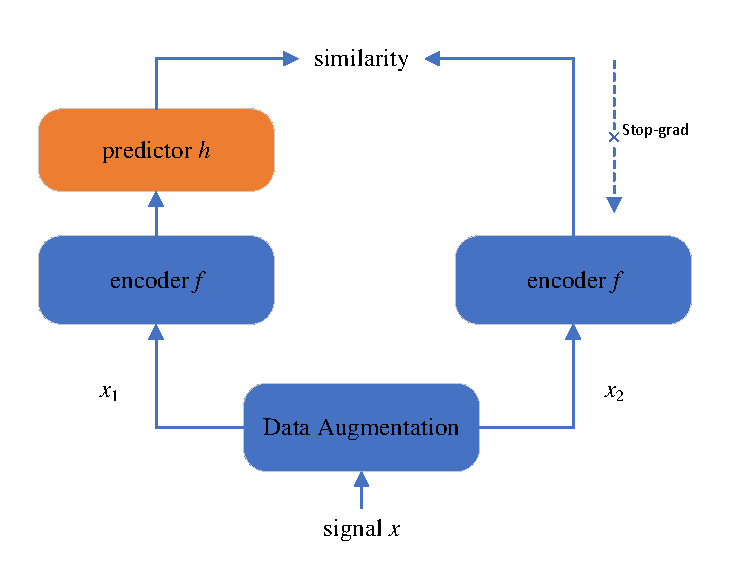
\includegraphics[width=11cm]{simsiam_arch.pdf}
    \caption{简单暹罗孪生网络}
    \label{simsiam_arch}
\end{figure}

\begin{table}
    \caption{{\CJKfamily{song}简单暹罗孪生网络的伪代码,用Pytorch描述}}
    \begin{tabular}{@{}l@{}}
    \toprule
    \multicolumn{1}{@{}l@{}}{\textbf{{\CJKfamily{song}简单暹罗孪生网络Pytorch伪代码}}} \\
    \midrule
    \begin{lstlisting}[basicstyle=\fontspec{Times New Roman}, frame=none]
#f: 骨干网络 + 投影器 MLP
#h: 预测器 MLP
for x in loader:  # 加载一个包含 n 个样本的小批量数据 x
    x1, x2 = aug(x), aug(x)  # 随机数据增强
    z1, z2 = f(x1), f(x2)  # 投影,形状为 n-by-d
    p1, p2 = h(z1), h(z2)  # 预测,形状为 n-by-d
    L = D(p1, z2)/2 + D(p2, z1)/2  # 损失函数

    L.backward()  # 反向传播
    update(f, h)  # SGD 更新

def D(p, z):  # 负余弦相似度
    z = z.detach()  # 停止梯度
    p = normalize(p, dim=1)  # 对 p 进行 L2 归一化
    z = normalize(z, dim=1)  # 对 z 进行 L2 归一化
    return -(p * z).sum(dim=1).mean()  # 计算负余弦相似度
    \end{lstlisting} \\
    \bottomrule
    \end{tabular}
    \label{table:simsiam_code}
\end{table}

引入停止梯度的设计暗示了另一个潜在的优化问题正在被隐式解决。SimSiam 是一种类似于期望最大化(EM)算法的方法,隐式涉及两组变量并解决两个潜在的子问题。停止梯度操作的引入是为了引入额外的变量集。

考虑以下形式的损失函数:
\begin{equation}
\label{eq:loss}
\mathcal{L}(\theta,\eta)=\mathbb{E}_{x,\mathcal{T}}\left[\|\mathcal{F}_{\theta} (\mathcal{T}(x))-\eta_{x}\|^{2}_{2}\right].
\end{equation}
其中,$\mathcal{F}$ 是由 $\theta$ 参数化的网络,$\mathcal{T}$ 是数据增强,$x$ 是输入样本。期望 $\mathbb{E}[\cdot]$ 是对输入样本和数据增强的分布进行的。为了便于分析,这里使用均方误差 $\|\cdot\|^{2}_{2}$,如果向量是 $\ell_{2}$-归一化的,则等效于余弦相似度。暂时不考虑预测器,稍后再讨论。

在式(\ref{eq:loss})中,引入了另一组变量,记为 $\eta$。$\eta$ 的大小与输入样本数量成正比。直观上,$\eta_{x}$ 是输入样本 $x$ 的表示,下标 ${}_{x}$ 表示使用输入样本索引访问 $\eta$ 的子向量。$\eta$ 不一定是网络的输出;它是一个优化问题的参数。

通过这种形式化,考虑解决以下问题:
\begin{equation}
\label{eq:min_loss}
\min_{\theta,\eta}\mathcal{L}(\theta,\eta).
\end{equation}
这里的问题是针对 $\theta$ 和 $\eta$ 的。这种形式化类似于 KMeans 聚类。变量 $\theta$ 类似于聚类中心:它是编码器的可学习参数。变量 $\eta_{x}$ 类似于样本 $x$ 的分配向量(在 KMeans 中是一个 one-hot 向量),它是 $x$ 的表示。

同样类似于 KMeans,式(\ref{eq:min_loss})中的问题可以通过交替算法解决,固定一组变量并解决另一组变量。形式上,可以在以下两个子问题之间交替:
\begin{equation}
\label{eq:theta_subproblem}
\theta^{t} \leftarrow \arg\min_{\theta}\;\mathcal{L}(\theta,\eta^{t-1})
\end{equation}
\begin{equation}
\label{eq:eta_subproblem}
\eta^{t} \leftarrow \arg\min_{\eta}\;\mathcal{L}(\theta^{t},\eta)
\end{equation}
其中,$t$ 是交替的索引,“$\leftarrow$”表示赋值。

可以使用随机梯度下降(SGD)来解决子问题(\ref{eq:theta_subproblem})。停止梯度操作是一个自然的结果,因为梯度不会反向传播到 $\eta^{t-1}$,而 $\eta^{t-1}$ 在这个子问题中是一个常数。

子问题 (\ref{eq:eta_subproblem}) 可以独立地为每个 $\eta_{x}$ 求解。现在的问题是最小化$\mathbb{E}_{\mathcal{T}}\left[\|\mathcal{F}_{\theta^{t}}(\mathcal{T}(x))-\eta_{x} \|_{2}^{2}\right]$,其中期望是对数据增强 $\mathcal{T}$ 的分布进行的。由于使用均方误差,可以通过以下方式轻松求解:

\begin{equation}
\label{eq:eta_update}
\eta_{x}^{t}\leftarrow\mathbb{E}_{\mathcal{T}}\Big{[}\mathcal{F}_{\theta^{t}}( \mathcal{T}(x))\Big{]}.
\end{equation}
这表明 $\eta_{x}$ 被赋值为 $x$ 在数据增强分布上的平均表示。

SimSiam 可以通过在式(\ref{eq:theta_subproblem})和式(\ref{eq:eta_subproblem})之间进行一次交替来近似。首先,通过仅对数据增强采样一次(记为 $\mathcal{T}^{\prime}$)并忽略 $\mathbb{E}_{\mathcal{T}}[\cdot]$ 来近似式(\ref{eq:eta_update}):
\begin{equation}
\label{eq:eta_approx}
\eta_{x}^{t}\leftarrow\mathcal{F}_{\theta^{t}}(\mathcal{T}^{\prime}(x)).
\end{equation}
将其代入子问题 (\ref{eq:theta_subproblem}),得到:

\begin{equation}
\label{eq:theta_update}
\theta^{t+1}\leftarrow\arg\min_{\theta}\mathbb{E}_{x,\mathcal{T}}\Big{[}\big{\| }\mathcal{F}_{\theta}(\mathcal{T}(x))-\mathcal{F}_{\theta^{t}}(\mathcal{T}^{ \prime}(x))\big{\|}_{2}^{2}\Big{]}.
\end{equation}
现在 $\theta^{t}$ 在这个子问题中是一个常数,而 $\mathcal{T}^{\prime}$ 由于其随机性暗示了另一个视图。这种形式化展示了孪生网络架构。其次,如果通过一步 SGD 减少损失来实现式(\ref{eq:theta_update}),那么可以接近 SimSiam 算法:一个自然带有停止梯度操作的孪生网络。

根据定义,预测器 $h$ 期望最小化:
\begin{equation}
\mathbb{E}_{x}\Big{[}\big{\|}h(z_{1})-z_{2}\big{\|}_{2}^{2}\Big{]} 
\label{eq:target_of_h}
\end{equation}
其中,$z_i = \mathcal{F}(x_i)$,$x_i$表示输入$x$的第$i$个视图。$h$ 的最优解应满足:对于任何输入$x$, $h(z_{1})\!=\!\mathbb{E}_{z}[z_{2}]\!=\!\mathbb{E}_{\mathcal{T}}\big{[}\mathcal{F}( \mathcal{T}(x))\big{]}$ 。这个项类似于式(\ref{eq:eta_update})中的项。在式(\ref{eq:eta_approx})的近似中,期望 $\mathbb{E}_{\mathcal{T}}[\cdot]$ 被忽略了。$h$ 的使用可能填补了这一空白。在实践中,实际计算期望 $\mathbb{E}_{\mathcal{T}}$ 是不现实的。但神经网络(例如预测器 $h$)可能能够学习预测期望,而 $\mathcal{T}$ 的采样隐式分布在多个 epoch 中。

根据上述讨论,$h$ 的最优解应满足 $h(z_1) = E_z[z_2]$。假设 $h$ 为线性映射,则有 $h(E[z_1]) = E[z_2]$。同时,根据对称损失函数式~(\ref{eq:cos_loss}),$h$ 的最优解应满足 $h(z_2) = E_z[z_1]$。将此关系代入,得到 $h(E[z_1]) = E[z_2]$,进一步推导得 $h(h(z_2)) = E[z_2]$。因此,可表示为:
\begin{equation}
    h(h(x)) = E[x]
    \label{eq:derivation_of_h}
\end{equation}

这表明,在满足最优解的条件下,$h$ 很可能是输入变量 $x$ 到其期望值的平滑映射。假设 $h = E$,显然这是式~(\ref{eq:derivation_of_h}) 的一个特解。基于此,子问题~(\ref{eq:theta_subproblem}) 可以表述为:

\begin{equation}
    \arg\min_{\theta} \left[\| \mathcal{F}_{\theta}(x_1) - E(z_2) \|_2^2 + \| \mathcal{F}_{\theta}(x_2) - E(z_1) \|_2^2 \right]
\end{equation}

因此,SimSiam 的目标是最小化两个视图 \( x_1 \) 和 \( x_2 \) 输出特征期望值之间的距离,即使得 \( E(\mathcal{F}_\theta(x_1)) = E[z_2] \) 且 \( E(\mathcal{F}_\theta(x_2)) = E[z_1] \),从而促使模型学习到在数据增强下保持不变的深层次语义。图~\ref{simsiam_derivation_of_features} 直观展示了模型训练前后特征分布的变化。在训练前,多个相似样本的两个视图的特征在特征空间中可能位于距离较远且形态各异的区域;而在训练后,两个视图的特征空间趋于重叠,且期望值之间的距离显著缩小。这表明,编码器成功学习到了对数据增强不敏感的深层次语义特征。此时,当 \( h \) 计算出 \( E[z_1] \) 时,即可得到式~(\ref{eq:target_of_h}) 的最优解,对于 \( z_2 \) 同理。

然而,如果数据增强模块没有有效地带来多样化的特征空间分布(例如,训练前两个视图的特征空间已经趋于重叠),那么当 \( h \) 学习到预测期望的能力时,编码器可能不再需要进一步学习那些与数据增强无关的深层语义特征。

\begin{figure}[h]
    \centering
    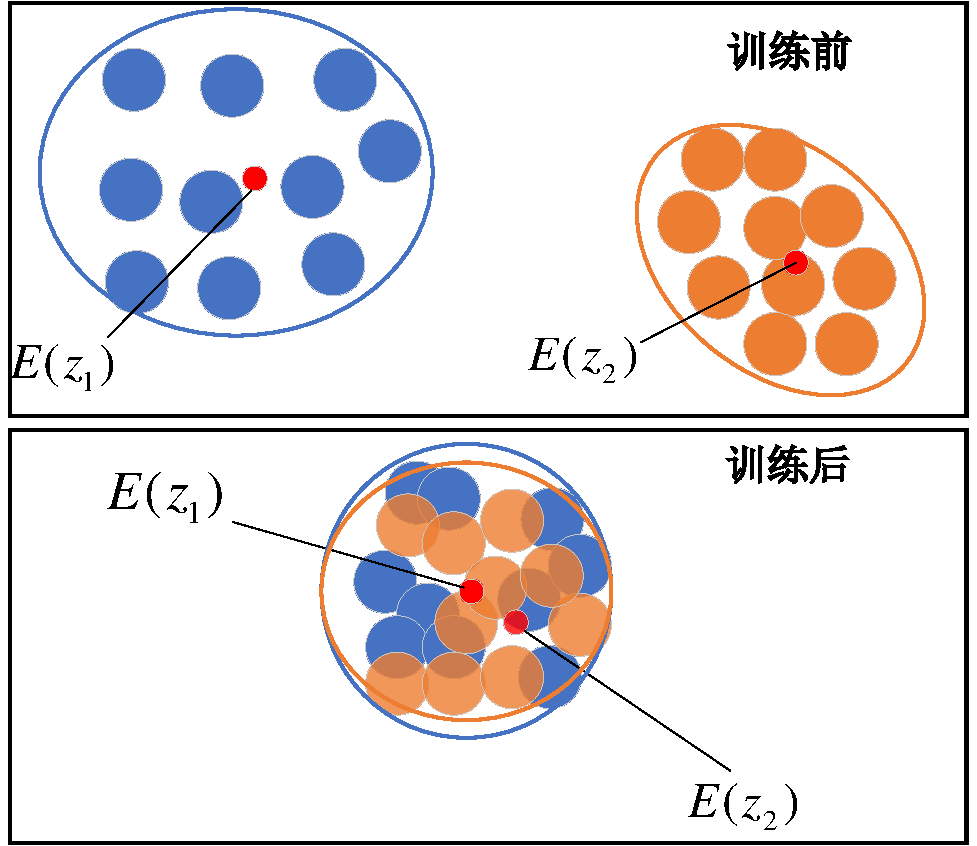
\includegraphics[width=8cm]{simsiam_derivation_of_features.pdf}
    \caption{不同视图的模型特征输出分布的变化示意图}
    \label{simsiam_derivation_of_features}
\end{figure}

\section{特征可视化与优化方法理论基础}
\subsection{t-SNE降维原理}
t-SNE,全称为 t 分布随机邻域嵌入,是一种被广泛应用的非线性降维方法,常用于将高维数据映射到二维或三维空间,以便借助散点图直观展示数据的分布特征和聚类结构。该方法在图像识别、文本分析和高维特征可视化等任务中表现出色,能够有效揭示数据在低维空间中的内在结构。

t-SNE 的降维过程可以概括为三个主要环节。首先,在高维空间中,t-SNE 计算任意两点之间的相似度。对于每对数据点,其相似度通过条件概率表示,其中任意两个数据点 \(x_i\) 和 \(x_j\) 的相似度 \(p_{ij}\) 定义如下:

\begin{equation}
p_{ij} = \frac{\exp\left( -\frac{\|x_i - x_j\|^2}{2\sigma_i^2} \right)}{\sum_{j \neq i} \exp\left( -\frac{\|x_i - x_j\|^2}{2\sigma_i^2} \right)}
\end{equation}

其中,\(\|x_i - x_j\|\) 表示两点之间的欧氏距离,\(\sigma_i\) 是与数据点 \(x_i\) 相关的局部尺度参数,用于控制其邻域范围。这种方式确保了模型在高维空间中对每个点的局部结构进行精确建模,从而更好地反映数据的分布特性。

接下来,t-SNE 将数据映射到低维空间,并在该空间中重新计算数据点之间的相似度。与高维空间中采用的高斯分布不同,t-SNE 在低维空间中采用 t 分布来定义点之间的相似度,计算公式如下:

\begin{equation}
q_{ij} = \frac{\left( 1 + \|y_i - y_j\|^2 \right)^{-1}}{\sum_{j \neq i} \left( 1 + \|y_i - y_j\|^2 \right)^{-1}}
\end{equation}

其中,\(y_i\) 和 \(y_j\) 分别表示低维空间中的数据点向量,\(\|y_i - y_j\|\) 是它们之间的欧氏距离。t 分布的重尾特性可以有效缓解低维空间中的“拥挤问题”,使得不同簇之间的距离得以清晰拉开,从而增强聚类结构的可视化效果。

为了尽可能保持高维空间中的数据相似度关系,t-SNE 通过最小化高维与低维之间的相似度分布差异来优化嵌入过程。这一优化目标通过 Kullback-Leibler 散度进行度量,其定义如下:

\begin{equation}
\text{KL}(P || Q) = \sum_{i,j} p_{ij} \log \frac{p_{ij}}{q_{ij}}
\end{equation}

其中 \(P\) 表示高维空间的相似度分布,\(Q\) 表示低维空间的相似度分布。通过反复迭代优化,t-SNE 会不断调整低维空间中各数据点的位置,使得两种分布之间的差异最小化,从而实现高质量的降维可视化。

综上所述,t-SNE 以其在保持局部结构、突出聚类特征以及适应复杂分布等方面的优势,已成为高维数据可视化领域中不可或缺的重要工具。

t-SNE降维伪代码见表\ref{table:tsne_code}。
\begin{table}[h]
    \caption{{\CJKfamily{song}t-SNE算法伪代码}}
    {\CJKfamily{song} % 只让这个表格内容中文是宋体
    \begin{tabular}{@{}l@{}} % 去左右边距,左对齐
    \toprule
    \multicolumn{1}{@{}l@{}}{\textbf{t-SNE算法伪代码}} \\
    \midrule
    \begin{lstlisting}[basicstyle=\fontspec{Times New Roman}, frame=none]
# 输入: 高维数据 X = {x1, x2, ..., xn}
# 输出: 低维数据 Y = {y1, y2, ..., yn}
# Step 1: 计算高维空间中数据点之间的相似度 p_ij
for i = 1 to n:  # 对每个数据点 xi
    for j = 1 to n:
        # 计算 xi 和 xj 之间的欧氏距离,并转化为条件概率 p_ij
        dist_ij = norm(xi - xj)
        p_ij = exp(-dist_ij^2 / (2 * sigma_i^2)) / \
               sum(exp(-dist_ij^2 / (2 * sigma_i^2)) for all j)
        P[i][j] = p_ij  # 存储 p_ij    
# Step 2: 初始化低维空间中的数据点 Y
Y = random_initialization(n, d)  # 随机初始化低维空间中的数据点
# Step 3: 迭代优化:最小化KL散度
for t = 1 to T:  # 最大迭代次数 T
    # 计算低维空间中的相似度 q_ij
    for i = 1 to n:
        for j = 1 to n:
            dist_ij = norm(yi - yj)
            q_ij = (1 + dist_ij^2)^(-1) / \
                   sum((1 + dist_ij^2)^(-1) for all j)
            Q[i][j] = q_ij  # 存储 q_ij

    # 计算KL散度并计算梯度
    KL = sum(P[i][j] * log(P[i][j] / Q[i][j]) for all i and j)
    gradients = compute_gradients(P, Q, Y)  # 计算梯度    
    # Step 4: 更新低维空间中的数据点 Y
    Y = Y - learning_rate * gradients  # 梯度下降更新低维数据点
    # Step 5: 终止条件判断
    if converged(KL):  # 如果KL散度收敛
        break
return Y  # 返回降维后的低维数据 Y
    \end{lstlisting} \\
    \bottomrule
    \end{tabular}
    }
    \label{table:tsne_code}
\end{table}
\FloatBarrier  % 阻止后续浮动体越过这条线

\subsection{K-Means聚类原理}
K-Means 是一种经典的无监督学习算法,其核心思想是通过最小化样本点与各自簇中心之间的距离,将数据划分为 K 个簇。该算法在图像分割、客户细分、文档聚类以及特征提取等多个领域被广泛应用。算法步骤如下:
K-Means 是一种经典的无监督学习算法,其核心思想是通过最小化样本点与各自簇中心之间的距离,将数据划分为 \(K\) 个簇。该方法在图像分割、客户细分、文档聚类、特征提取等多个应用场景中被广泛采用。K-Means 的整体流程包括初始化、簇分配、质心更新、重复迭代以及标签匹配等步骤。

K-Means 算法的伪代码如表~\ref{table:kmeans_code} 所示,清晰展示了其基本流程与实现逻辑。

\begin{table}[h]
    \caption{{\CJKfamily{song}KMeans算法伪代码}}
    {\CJKfamily{song}
    \begin{tabular}{@{}l@{}}
    \toprule
    \multicolumn{1}{@{}l@{}}{\textbf{KMeans算法伪代码}} \\
    \midrule
    \begin{lstlisting}[basicstyle=\fontspec{Times New Roman}, frame=none]
# 输入: 数据集 X = {x1, x2, ..., xn}, 簇数 K, 最大迭代次数 T
# 输出: 簇标签 {y1, y2, ..., yn}

# 初始化:随机选择 K 个数据点作为初始质心 C = {c1, c2, ..., cK}
for t = 1 to T:  # 最大迭代次数 T
    for i = 1 to n:  # 对每个数据点 xi
        # 计算每个质心的距离,分配数据点给最近的质心
        distances = []  # 初始化一个空列表
        for cj in C:  # 对每个质心 cj
            dist = norm(xi - cj)  # 计算 xi 到 cj 的距离
            distances.append(dist)  # 添加到距离列表
        yi = argmin(distances)  # 分配数据点 xi 到最近的质心
        # 更新数据点的簇标签
        labels[i] = yi
    
    for j = 1 to K:  # 对每个簇
        # 更新质心为簇中所有数据点的均值
        cluster_points = 
            [xi for xi, label in zip(X, labels) if label == j]
        # 计算簇内数据点的均值作为新质心
        C[j] = mean(cluster_points)
    
    # 使用匈牙利算法找到最佳匹配
    optimal_labels = hungarian_algorithm(labels, C)
    
    # 如果质心不再变化
    if no_change_in_centroids(C):  # 如果质心不再变化
        break  # 退出

return optimal_labels  # 返回优化后的簇标签 {y1, y2, ..., yn}
    \end{lstlisting} \\
    \bottomrule
    \end{tabular}
    }
    \label{table:kmeans_code}
\end{table}

在初始阶段,算法从数据集中随机选取 \(K\) 个样本作为初始簇中心。随后,依据最小欧氏距离准则,将每个数据点 \(x_i\) 分配给距离其最近的簇中心 \(c_j\)。两者之间的欧氏距离计算方式如下:

\begin{equation}
\text{Distance}(x_i, c_j) = \| x_i - c_j \|
\end{equation}

完成分配后,算法会重新计算每个簇的质心,即簇内所有数据点的均值,更新公式如下:

\begin{equation}
c_j = \frac{1}{|S_j|} \sum_{x_i \in S_j} x_i
\end{equation}

其中,\(S_j\) 表示第 \(j\) 个簇中的样本集合,\(|S_j|\) 是该簇中样本的数量。簇分配与质心更新这两个步骤不断交替进行,直至簇质心收敛,或达到设定的最大迭代次数为止。

在聚类迭代完成后,为了优化簇标签与真实标签之间的对应关系,可引入匈牙利算法来实现最优匹配。该算法能够最小化聚类标签与真实标签之间的总匹配成本,从而提高聚类评估的一致性与准确性。
\FloatBarrier  % 阻止后续浮动体越过这条线


\subsection{协方差矩阵适应进化策略原理}
协方差矩阵适应进化策略(Covariance Matrix Adaptation Evolution Strategy,CMA-ES)是一种用于连续域全局优化的进化算法。它采用基于种群的搜索机制,通过不断更新搜索分布的均值、步长和协方差矩阵来引导优化过程,尤其擅长处理非线性、非凸、高维的复杂问题。CMA-ES 广泛应用于机器学习中的超参数优化、工程设计以及复杂系统建模等任务中,因其鲁棒性和自适应能力而受到广泛关注。

在每一代中,CMA-ES 首先通过采样生成候选解。候选解的生成方式如下:

\begin{equation}
\mathbf{x}_k^{(g+1)} = \mathbf{m}^{(g)} + \sigma^{(g)} \cdot \mathcal{N}(0, \mathbf{C}^{(g)})
\label{eq:sample}
\end{equation}

其中,\(\mathbf{x}_k^{(g+1)}\) 表示第 \(g+1\) 代中的第 \(k\) 个候选解,\(\mathbf{m}^{(g)}\) 是当前种群的均值向量,\(\sigma^{(g)}\) 为当前步长控制参数,\(\mathbf{C}^{(g)}\) 是协方差矩阵,\(\mathcal{N}(0, \mathbf{C}^{(g)})\) 表示从零均值、协方差为 \(\mathbf{C}^{(g)}\) 的多元正态分布中采样的扰动向量。

随后,根据适应度函数对候选解进行排序,选取前 \(\mu\) 个最优个体来更新新的均值。更新公式如下:

\begin{equation}
\mathbf{m}^{(g+1)} = \sum_{i=1}^{\mu} w_i \mathbf{x}_{i:\lambda}^{(g+1)}
\label{eq:mean_update}
\end{equation}

其中,\(w_i\) 是各候选解的权重系数,\(\mathbf{x}_{i:\lambda}^{(g+1)}\) 表示按照适应度排序后的第 \(i\) 个候选解。

协方差矩阵的更新机制考虑了两个因素:一是路径累计项用于捕捉连续迭代方向上的长期信息,二是基于当前最优样本的分布信息修正协方差结构。更新规则如下所示:

\begin{equation}
\mathbf{C}^{(g+1)} = (1 - c_1 - c_\mu) \mathbf{C}^{(g)} + c_1 \mathbf{p}_c^{(g+1)} (\mathbf{p}_c^{(g+1)})^\top + c_\mu \sum_{i=1}^{\mu} w_i \mathbf{y}_{i:\lambda}^{(g+1)} (\mathbf{y}_{i:\lambda}^{(g+1)})^\top
\label{eq:covariance_update}
\end{equation}

其中,\(\mathbf{p}_c^{(g+1)}\) 是协方差路径,\(\mathbf{y}_{i:\lambda}^{(g+1)} = (\mathbf{x}_{i:\lambda}^{(g+1)} - \mathbf{m}^{(g)}) / \sigma^{(g)}\),而 \(c_1\) 与 \(c_\mu\) 是控制学习率的常数项。

最后,为了进一步控制搜索范围的尺度,CMA-ES 对步长 \(\sigma\) 进行自适应调整,其更新规则如下:

\begin{equation}
\sigma^{(g+1)} = \sigma^{(g)} \exp\left(\frac{c_\sigma}{d_\sigma} \left(\frac{\|\mathbf{p}_\sigma^{(g+1)}\|}{\mathbb{E}[\|\mathcal{N}(0, \mathbf{I})\|]} - 1\right)\right)
\label{eq:stepsize_update}
\end{equation}

其中,\(\mathbf{p}_\sigma^{(g+1)}\) 是步长进化路径,\(c_\sigma\) 和 \(d_\sigma\) 分别表示步长的学习率和阻尼系数,\(\mathbb{E}[\|\mathcal{N}(0, \mathbf{I})\|]\) 是单位高斯分布下向量范数的期望值。

综上所述,CMA-ES 通过协方差矩阵与步长的动态调整,使得算法能够在复杂优化空间中自适应地寻找搜索方向与尺度,兼顾探索与收敛,是解决连续优化问题的强有力工具之一。

\FloatBarrier  % 阻止后续浮动体越过这条线


\section{数据集介绍}
\subsection{凯斯西储大学 CWRU数据集}
所使用的数据集由凯斯西储大学(Case Western Reserve University)提供。图 \ref{cwru_device} 展示了该实验平台的结构配置,其主要包括一台 2 马力的电动机、扭矩编码器、测功机及若干控制电路。实验中使用的轴承为 6205-2RS JEM 型深沟球轴承,分别安装在电机的驱动端和风扇端位置。

轴承故障是通过单点电火花放电加工(Electro-discharge Machining)制造的。根据故障位置,故障类型可分为以下四种:  
外圈故障(Outer Raceway Fault, OF);  
内圈故障(Inner Raceway Fault, IF);  
滚动体故障(Roller Faults, RFs);  
正常状态(Normal Condition, NC)。  
轴承故障的严重程度可由故障直径(Fault Diameter)描述,故障直径指轴承或其他机械部件上出现的故障或损伤的直径尺寸。 故障直径通常用来描述故障的大小和程度,对于故障诊断和预测维护非常重要。故障分类见表\ref{tab:cwru_fault_types}。
\begin{table}[H]
    \centering
    \caption{CWRU 轴承数据集故障类型表,其中0为正常类}
    \renewcommand\arraystretch{1.2}
    \begin{tabular}{ccc}
        \toprule
        序号 & 损伤部位 & 损伤直径 (mm) \\
        \midrule
        0  & - & - \\        
        1  & 外圈OF & 0.007 \\
        2  & 外圈OF & 0.014 \\
        3  & 外圈OF & 0.021 \\
        4  & 内圈IF & 0.007 \\
        5  & 内圈IF & 0.014 \\
        6  & 内圈IF & 0.021 \\
        7  & 滚珠BF & 0.007 \\
        8  & 滚珠BF & 0.014 \\
        9  & 滚珠BF & 0.021 \\
        \bottomrule
    \end{tabular}
    \label{tab:cwru_fault_types}
\end{table}

本研究采集了驱动端轴承的数据,采样频率为 12 kHz,故障类型包括内圈故障、外圈故障和滚动体故障,故障直径分别为 0.007 英寸、0.014 英寸和 0.021 英寸。不同故障类型的波形如图 \ref{cwru_samples} 所示。有关该数据集的更多详细信息,可访问 CWRU 轴承数据中心网站\citing{loparo2012case}。  

\begin{figure}[h]
    \centering
    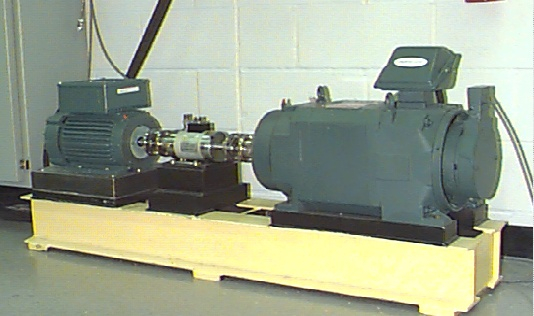
\includegraphics[width=6cm]{cwru_device.jpeg}
    \caption{CWRU轴承测试设备}
    \label{cwru_device}
\end{figure}

\begin{figure}
    \centering
    \subfloat[]{
        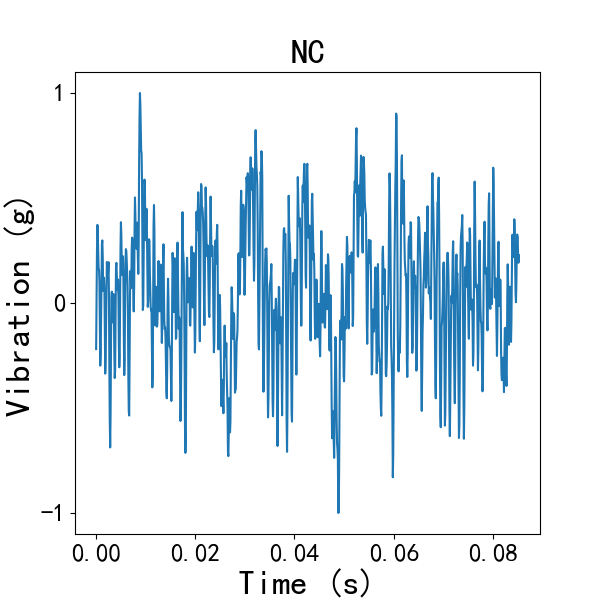
\includegraphics[width=0.28\linewidth]{class_0.png}
        \label{class_0}
    }
    \subfloat[]{
        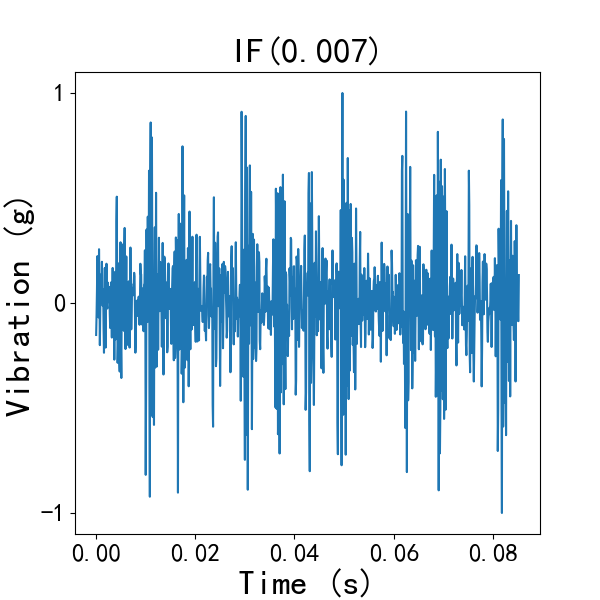
\includegraphics[width=0.28\linewidth]{class_1.png}
        \label{class_1}
    }
    \subfloat[]{
        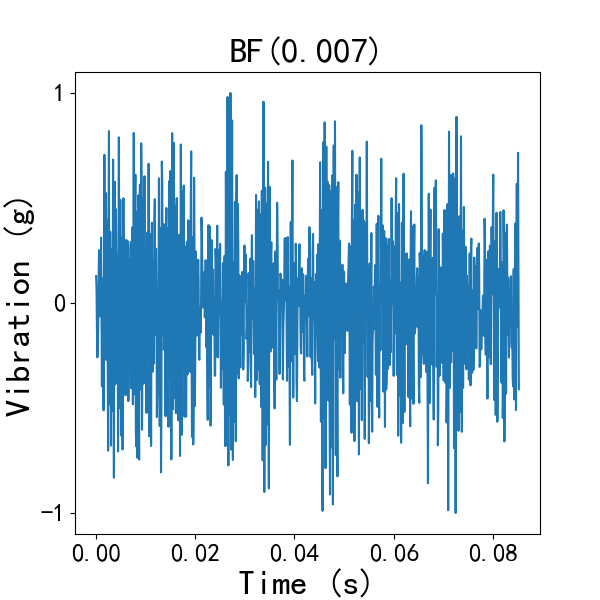
\includegraphics[width=0.28\linewidth]{class_2.png}
        \label{class_2}
    }
    \\ % 换行
    \subfloat[]{
        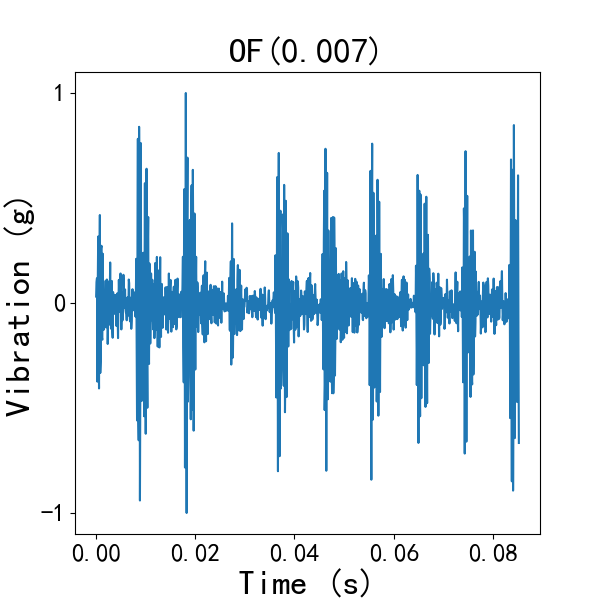
\includegraphics[width=0.28\linewidth]{class_3.png}
        \label{class_3}
    }
    \subfloat[]{
        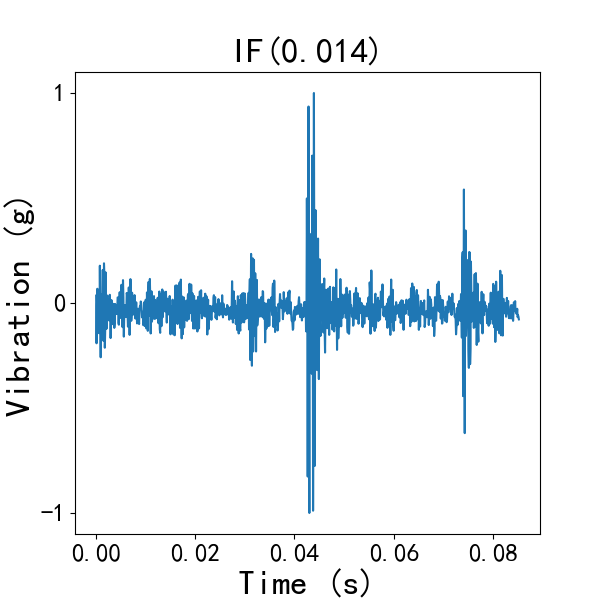
\includegraphics[width=0.28\linewidth]{class_4.png}
        \label{class_4}
    }
    \subfloat[]{
        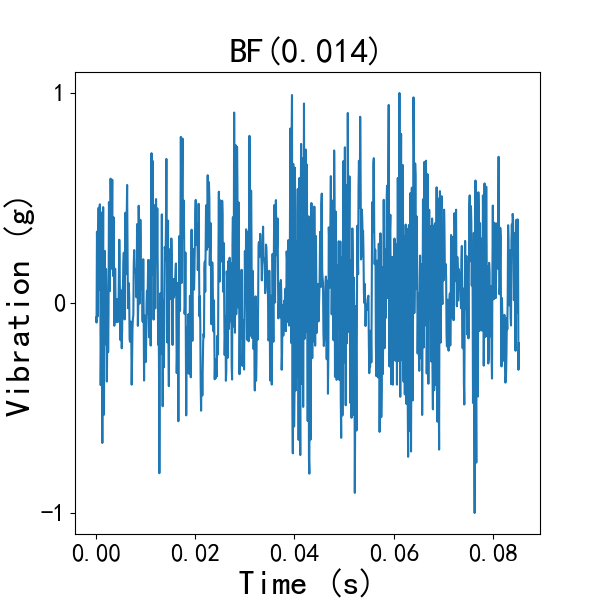
\includegraphics[width=0.28\linewidth]{class_5.png}
        \label{class_5}
    }
    \\ % 换行
    \subfloat[]{
        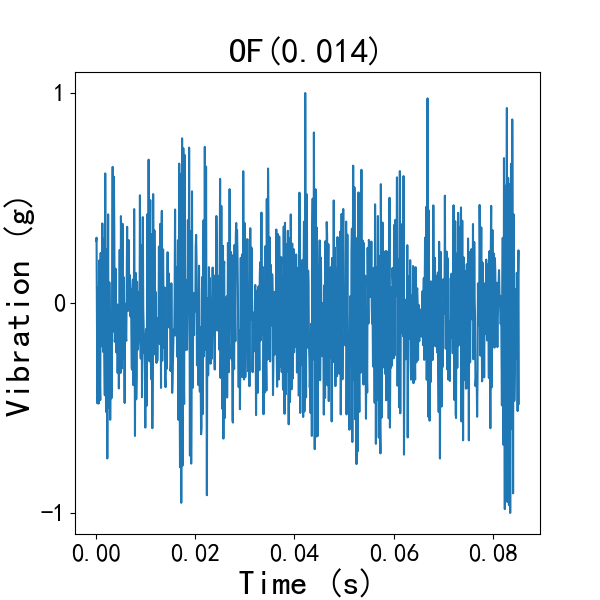
\includegraphics[width=0.28\linewidth]{class_6.png}
        \label{class_6}
    }
    \subfloat[]{
        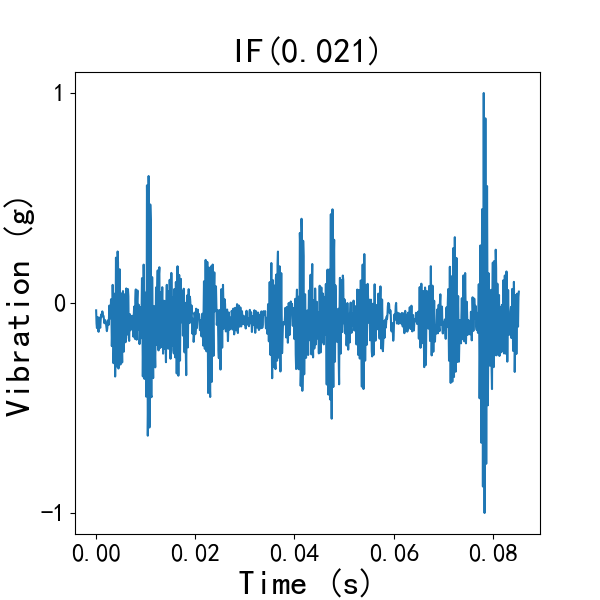
\includegraphics[width=0.28\linewidth]{class_7.png}
        \label{class_7}
    }
    \subfloat[]{
        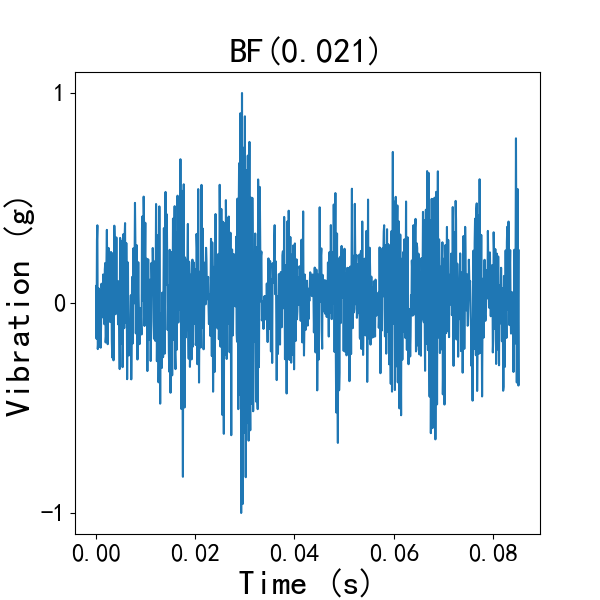
\includegraphics[width=0.28\linewidth]{class_8.png}
        \label{class_8}
    }
    \\ % 换行
    \subfloat[]{
        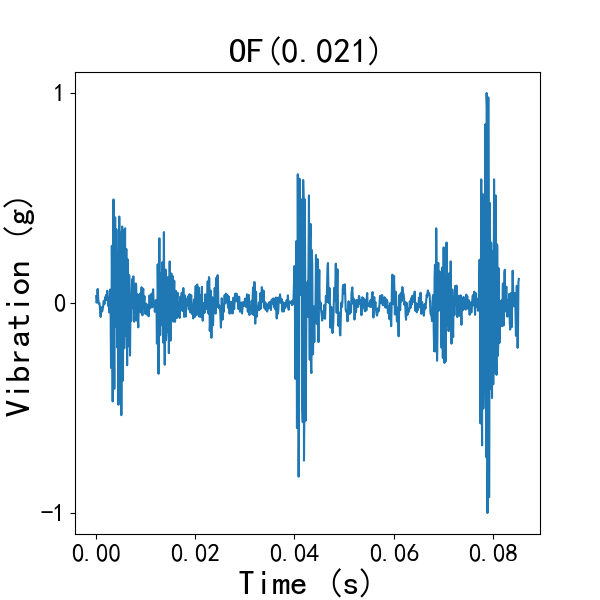
\includegraphics[width=0.28\linewidth]{class_9.png}
        \label{class_9}
    }

    \caption{每个类别的样本信号示例:\textbf{(a)} NC;\textbf{(b)} IF(0.007);\textbf{(c)} BF(0.007)  \textbf{(d)} OF(0.007);\textbf{(e)} IF(0.014);\textbf{(f)} BF(0.014);\textbf{(g)} OF(0.014);\textbf{(h)} IF(0.021);\textbf{(i)} BF(0.021);\textbf{(j)} OF(0.021)}
    \label{cwru_samples}
\end{figure}
\FloatBarrier  % 阻止后续浮动体越过这条线

\subsection{帕德伯恩大学PU数据集}
PU轴承试验台由电机、测矩轴、滚动轴承试验模块、飞轮和负载电机组成,所有测试轴承均为6203型号滚动轴承。故障类别以不同损伤部位、损伤程度、损伤方法区分,加上正常类,共13类,具体故障类型如表\ref{tab:pu_fault_types}所示。
\begin{table}[H]
    \centering
    \caption{PU数据集故障类型分类表,其中0为正常类}
    \renewcommand\arraystretch{1.2}
    \begin{tabular}{ccccccc}
        \toprule
        序号 & 轴承编码 & 制造商 & 损伤程度 & 损伤部位 & 损伤方法 \\
        \midrule
        0  & K001 & IBU & - & - & - \\
        1  & KA01 & MTK & 1 & 外圈 & 电火花加工 \\
        2  & KA03 & LBU & 2 & 外圈 & 电雕刻 \\
        3  & KA05 & LBU & 1 & 外圈 & 电雕刻 \\
        4  & KA06 & LBU & 2 & 外圈 & 电雕刻 \\
        5  & KA07 & LBU & 1 & 外圈 & 转孔 \\
        6  & KA08 & LBU & 2 & 外圈 & 转孔 \\
        7  & KA09 & LBU & 2 & 外圈 & 转孔 \\
        8  & KI01 & MTK & 1 & 内圈 & 电火花加工 \\
        9  & KI03 & LBU & 1 & 内圈 & 电雕刻 \\
        10 & KI05 & LBU & 1 & 内圈 & 电雕刻 \\
        11 & KI07 & LBU & 2 & 内圈 & 电雕刻 \\
        12 & KI08 & LBU & 2 & 内圈 & 电雕刻 \\
        \bottomrule
    \end{tabular}
    \label{tab:pu_fault_types}
\end{table}

\subsection{长尾数据集构造}
模拟构建长尾分布数据集流程如图~\ref{pareto}所示。设定不平衡因子 \(\beta = x_{\text{max}} / x_{\text{min}}\) 为数据集中样本数量最多的类与样本数量最少的类的数量之比。帕累托分布的概率密度函数为 \(p(x) = \frac{\alpha x_{\text{min}}^{\alpha}}{x^{\alpha+1}}\),令$x_{\text{min}} = 1$,则\(p(x) = \frac{\alpha}{x^{\alpha+1}}\)。以不平衡因子构建服从帕累托分布的长尾分布数据集,不同不平衡因子的帕累托分布概率密度函数如图~\ref{paerto_fig_beta}所示,可以看到当最大类与最小类样本数的比值 \(\beta\) 增大时,帕累托分布的形状参数 \(\alpha\) 也随之增大。这表明分布的头部类别占比提高,而尾部类别占比显著降低,长尾效应越发显著。下面将介绍形状参数 \(\alpha\) 的求解方法,以及各类别样本占比的计算步骤。

\begin{figure}[h]
    \centering
    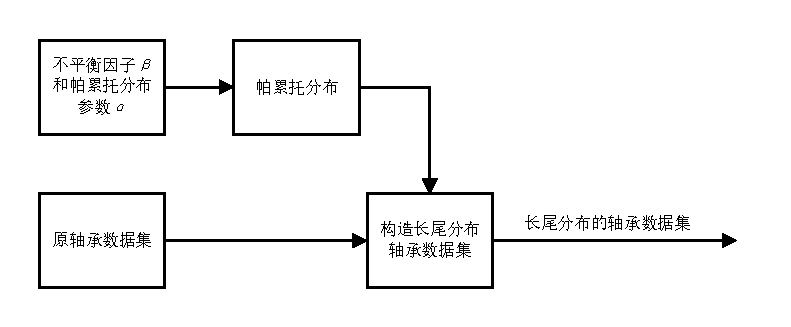
\includegraphics[width=11cm]{pareto.pdf}
    \caption{基于帕累托分布构造长尾分布的轴承数据集流程图}
    \label{pareto}
\end{figure}

\begin{figure}[h]
    \centering
    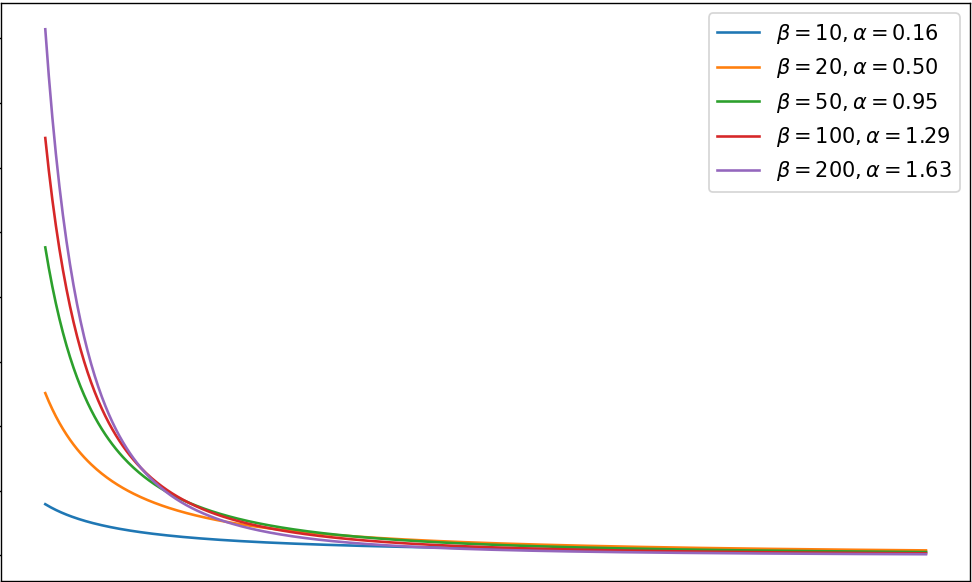
\includegraphics[width=12cm]{paerto_fig_beta.png}
    \caption{不同不平衡因子$\beta$的帕累托分布概率密度图}
    \label{paerto_fig_beta}
\end{figure}

已知帕累托分布的累积分布函数为:
\begin{equation}
F(x) = 1 - x^{-\alpha}, \quad x > 1
\end{equation}

每类的概率定义为:
\begin{equation}
P(n \leq x < n+1) = F(n+1) - F(n) = n^{-\alpha} - (n+1)^{-\alpha}
\end{equation}

设最大类与最小类的样本数比值为 $\beta$,则有以下关系式:
\begin{equation}
\beta = \frac{P(1 \leq x < 2)}{P(n \leq x < n+1)} = \frac{1 - 2^{-\alpha}}{n^{-\alpha} - (n+1)^{-\alpha}}
\end{equation}

目标是
    根据给定的 $\beta$ 和类别总数 $n$,求解形状参数 $\alpha$。
    其次计算每类的样本占比 $P(n \leq x < n+1)$。
    最后将所有类别的概率归一化,使其和为 1。
具体步骤如下:
    
首先求解 $\alpha$,根据 $\beta$ 的定义,解以下非线性方程以确定 $\alpha$:
\begin{equation}
\beta = \frac{1 - 2^{-\alpha}}{n^{-\alpha} - (n+1)^{-\alpha}}
\end{equation}
该方程一般无解析解,可以通过数值方法(如 Newton-Raphson 或其他优化算法)求解。

其次计算每类的概率,每类的概率可以通过以下公式计算:
\begin{equation}
P(n \leq x < n+1) = n^{-\alpha} - (n+1)^{-\alpha}, \quad n = 1, 2, \dots, N
\end{equation}

最后概率归一化,将所有类别的概率归一化,计算归一化后的概率:
\begin{equation}
P_{\text{norm}}(n \leq x < n+1) = \frac{P(n \leq x < n+1)}{\sum_{k=1}^N P(k \leq x < k+1)}
\label{pareto_sample}
\end{equation}
其中 $N$ 为类别总数,归一化后各类别的样本占比之和为 1:
\begin{equation}
\sum_{n=1}^N P_{\text{norm}}(n \leq x < n+1) = 1
\end{equation}

\section{本章小结}
本章系统地介绍了自监督学习的相关理论基础,重点分析了孪生网络与对比学习在特征提取中的关键作用,明确了其在无监督条件下实现语义聚合的优势,同时在理论上分析了孪生网络训练的过程。同时,本章还阐述了用于可视化与聚类分析的 t-SNE 降维算法与 K-Means 聚类原理,为后续特征可视化和聚类评价提供了理论支撑。此外,还对协方差矩阵适应进化策略(CMA-ES)的基本原理进行了简要说明,作为后续优化方法的理论依据。最后,本章详细介绍了实验中使用的轴承故障数据集,包括凯斯西储大学 CWRU 数据集、帕德伯恩大学 PU 数据集,并提出了一种基于帕累托分布的长尾数据集构造方法,为后续验证模型在不平衡样本条件下的性能奠定了数据基础。

\chapter{基于自适应数据增强优化的对比学习故障诊断网络}
在智能制造与设备健康管理领域,针对长尾分布问题,常见的解决方案之一是先通过对比学习训练模型的特征提取层,再训练分类器层。这种方法能够使特征提取层学习到更加鲁棒的特征表示,从而为分类器层的训练提供更加有效的输入。尤其在处理长尾分布数据时,特征提取层的优化尤为关键,因为它直接影响模型对少数类样本的判别能力。

然而,在实际应用中,孪生网络对比学习容易出现“特征坍塌”(representation collapse)现象,即网络输出趋于某种平凡解,导致提取的特征缺乏判别性,从而影响模型性能和泛化能力。

为缓解这一问题,已有研究通过引入投影头、构造负样本对等方式来增强模型的稳定性。但在实际场景中,故障数据往往存在分布不均衡、标签不足等问题,依赖结构调整手段仍难以充分挖掘样本的判别信息。因此,合理的数据增强策略有望在提升特征表达能力方面发挥更为直接的作用,成为改善对比学习效果的关键因素之一。包括基于长短时记忆网络(LSTM)的强化学习方法~\citing{cubuk2018autoaugment}、数据分布密度匹配的贝叶斯优化方法~\citing{lim2019fast},以及遗传算法。


基于此,本章在孪生网络对比学习的故障诊断网络基础上,设计并引入了一种自适应数据增强策略框架,旨在根据数据特征的质量评估自动调整增强模块的参数。该策略通过提升网络对关键故障特征的感知能力,进一步缓解特征坍塌问题。引入自适应数据增强策略后,基于数据增强模块生成样本对进行训练的对比学习模型能够更加灵活地调整特征提取层的学习过程,从而显著提升在长尾数据集上的判别能力。通过实验,本章对增强模块的作用进行了详细分析和验证,评估了其在诊断准确性和鲁棒性方面的影响。


\section{模型整体架构及其模块设计}
\subsection{基于自适应数据增强优化的对比学习故障诊断网络整体结构}

本章提出了一种基于自适应数据增强优化的对比学习故障诊断网络,其结构如图~\ref{simsiam_net}所示。模型训练分为三个阶段。首先,在自适应数据增强驱动的自监督对比学习阶段,原始无标签样本通过数据增强模块生成两个不同视图作为正样本对,输入孪生网络进行对比学习以优化编码器的特征表示能力。随后,编码器提取的特征向量经过特征质量评估模块,通常采用轮廓系数或有标签样本上的分类准确率作为质量指标 $Q$。该指标反馈至数据增强控制器,用以动态调整增强操作的执行概率 $p$ 和增强强度 $s$,实现增强策略的自适应优化。数据增强控制器的实现方式多样。


第二阶段为微调阶段,将第一阶段训练完成的编码器与线性分类层结合,在带标签样本上进行有监督训练。此外,线性分类层也可替换为其他分类器,如KNN或SVM。最后,在故障诊断阶段,将训练好的编码器与分类器组成完整的故障分类模型,应用于实际故障识别任务,实现高效准确的诊断。

以下小节将详细介绍各模块的具体实现细节。

\begin{figure}[h]
    \centering
    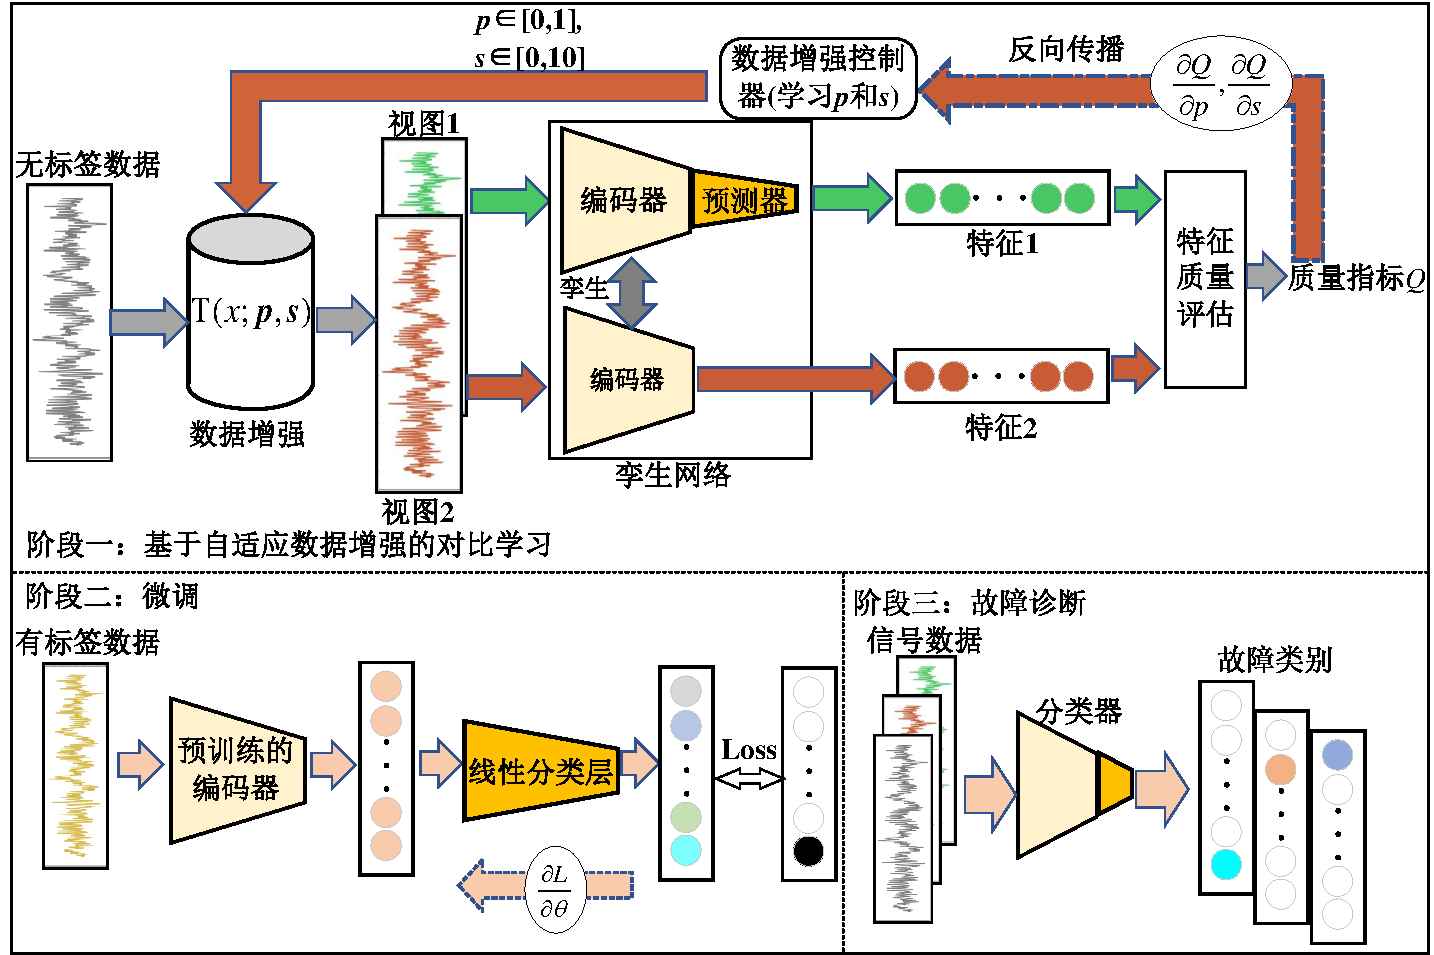
\includegraphics[width=15cm]{simsiam_net_aa.pdf}
    \caption{基于自适应数据增强优化的孪生故障诊断网络}
    \label{simsiam_net}
\end{figure}
\FloatBarrier  % 阻止后续浮动体越过这条线
\subsection{基于自适应数据增强的自监督对比学习}

对比学习是一种自监督学习方法,通过最大化正样本对之间的相似度并最小化负样本对之间的相似度,来学习有效的特征表示。具体来说,给定一个输入样本 $x$,通过数据增强操作生成多个不同的视图,如 $x_1, x_2$ 等。网络通过对比学习算法将这些视图映射到嵌入空间中,并尽量使得相同样本的视图(正样本对)之间的距离尽可能小,而不同样本的视图(负样本对)之间的距离尽可能大。最终,通过这种方式,模型能够学习到具有判别力的表示,使得相同类别的样本在嵌入空间中尽可能接近,而不同类别的样本尽可能远离。

在对比学习的应用中,数据增强起着至关重要的作用。编码器是否能从振动信号中成功提取可区分的故障特征,在很大程度上取决于数据增强策略的设计。当前,尽管图像领域的对比学习采用了多种数据增强方法,但针对时序数据(如振动信号)的增强手段相对较少。有效的数据增强方法不仅需要保证语义一致性,即噪声或变换不应改变样本的核心语义特征(如故障类别),还需要具备足够的多样性,以在特征空间中引入有效的变化,从而促进编码器学习到更具判别性的深层语义表示。传统的对比学习往往依赖于手工设计的增强策略,这些策略通常基于领域经验,但缺乏针对具体数据特征的适应性。一方面,固定策略难以保证在不同故障模式下的语义一致性;另一方面,手工设定的增强强度可能导致样本差异不足,从而限制判别特征的学习。

为此,本文引入了一个可学习的控制器,能够通过端到端优化自动调整增强操作的执行概率 $p$ 和增强强度 $s$,从而实现自适应的数据增强策略。该方法通过不断优化增强策略,提升特征表示的质量和判别能力。

如图~\ref{aa_module}所示,本文提出的自适应数据增强(AutoAugment)自监督对比学习框架包括以下步骤:首先,原始振动信号 $x$ 经由数据增强模块生成两个不同的视图 $x_1$ 和 $x_2$,这两个视图构成正样本对并输入到孪生网络进行对比学习。孪生网络分别提取这两个视图的特征表示 $z_1$ 和 $z_2$,并将这些表示传递给特征质量评估模块,评估当前增强策略下的特征提取效果。评估结果作为反馈输入到数据增强控制器,控制器根据反馈动态调整增强操作的执行概率 $p$ 和增强强度 $s$,不断优化数据增强策略。这个过程持续迭代,促使增强策略和特征表示的学习达到协同进化。

\begin{figure}[h]
    \centering
    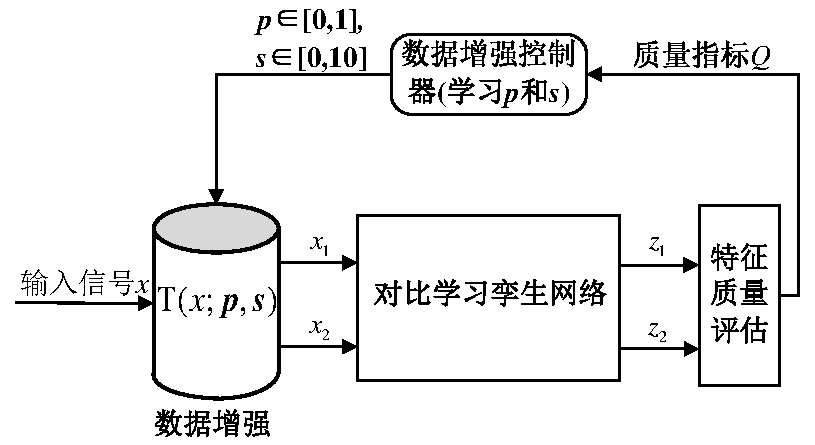
\includegraphics[width=10cm]{aa_module.pdf}
    \caption{自适应数据增强的对比学习框架图}
    \label{aa_module}
\end{figure}

数据增强模块由多个子策略组成,每个子策略由增强方法、应用概率 $p \in [0,1]$ 和增强强度 $s \in [0,10]$ 共同定义,旨在提升数据的多样性和模型的鲁棒性。本文采用了8种增强方法,详见表~\ref{tab:augmentation_descriptions},这些方法涵盖了高斯噪声、掩码、相位扰动、缩放等常见技术。图~\ref{data_augmentation}展示了不同增强方法对信号时域表现的影响,进一步揭示了各方法在实际应用中的有效性与差异。


\begin{table}[h]
    \caption{对比学习中使用的数据增强及强度映射}
    \centering
    \renewcommand\arraystretch{1.3}
    \begin{tabular}{clp{5cm}l} % 调整列宽,最后一列为自动宽度
    \toprule
    编号 & 增强方式 & 描述 & 强度映射 \\
    \midrule
    DA0 & 掩码 & 遮盖部分信号,增强鲁棒性 & 遮盖长度 $[1,5] \mapsto [0,10]$ \\
    DA1 & 高斯噪声 & 添加噪声,模拟干扰环境 & 信噪比 $[2,6] \mapsto [0,10]$ \\
    DA2 & 相位扰动 & 改变频域相位,保持幅值 & 相位幅度 $[0.1,0.5] \mapsto [0,10]$ \\
    DA3 & 块打乱 & 分块重排,提升多样性 & 块数 $[10,100] \mapsto [0,10]$ \\
    DA4 & 缩放 & 缩放幅度,模拟强弱变化 & 缩放比 $[0.05,0.6] \mapsto [0,10]$ \\
    DA5 & 绝对值 & 取正处理,统一极性 & -- \\
    DA6 & 竖直翻转 & 上下翻转,增强鲁棒性 & -- \\
    DA7 & 水平翻转 & 时间翻转,增加对称性 & -- \\
    \bottomrule
    \end{tabular}
    \label{tab:augmentation_descriptions}
\end{table}

\begin{figure}[H]
    \centering
    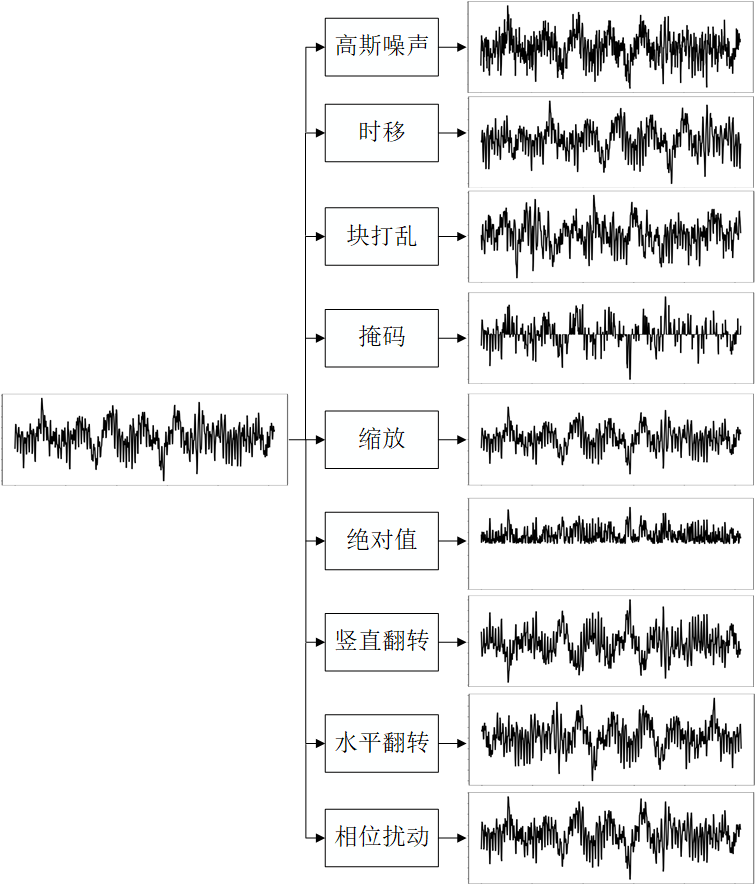
\includegraphics[width=10cm]{data_augmentation.png}
    \caption{数据增强方法效果示意图}
    \label{data_augmentation}
\end{figure}
特征质量评估模块衡量孪生网络编码器提取特征的有效性和判别能力,常用指标包括特征聚散度(同类特征聚合与异类特征分散程度)、KNN准确率、归一化互信息、调整兰德指数及轮廓系数等聚类指标。本文主要采用线性评估精度作为评价标准,即冻结编码器参数,训练线性分类器,并以其下游任务准确率衡量特征可分性,这有助于全面评估特征表示的质量和模型的泛化能力。

数据增强控制器作为框架核心模块,依据特征质量评估反馈动态调整各增强策略的执行概率 $p$ 和强度 $s$。训练过程中,控制器持续接收当前增强策略下特征质量指标,利用优化算法更新增强参数,实现增强策略自适应进化。此闭环机制有效引导数据增强向促进特征学习方向调整,提升无监督对比学习框架的表征能力及下游任务性能。控制器实现方式多样,常见包括基于长短时记忆网络的强化学习方法,将增强策略调整视作序列决策过程,通过强化学习最大化特征质量收益;基于数据分布密度匹配的贝叶斯优化方法,利用高斯过程建立增强参数与特征质量映射,通过采集函数引导全局搜索;以及遗传算法,通过编码增强参数为染色体,依靠选择、交叉与变异操作迭代优化种群,依据特征质量评价个体适应度,实现全局优化。本文采用遗传算法中的协方差矩阵自适应进化策略(CMA-ES)作为控制器实现,充分发挥其在非连续、非光滑优化问题中的优势,实现了数据增强参数的自适应学习与优化。


\subsection{基于预训练编码器的有监督微调}

在自监督对比学习阶段完成编码器的预训练后,为将模型迁移至具体的下游故障分类任务,本文采用了基于冻结特征提取器的初步微调策略。
微调过程中,我们固定预训练得到的编码器 $f(\cdot)$ 参数不变,仅在其输出后接入一个全连接分类器 $g(\cdot)$,其形式为:
\begin{equation}
    \hat{y} = \text{softmax}(g(f(x)))
\end{equation}
其中 $x$ 为输入样本,$f(x)$ 为提取的特征向量,$g(\cdot)$ 输出类别概率分布。

为了进行有监督分类训练,本文采用标准的交叉熵损失函数作为优化目标,其定义如下:
\begin{equation}
    \mathcal{L}_{\text{CE}} = - \sum_{i=1}^{C} y_i \log(\hat{y}_i)
\end{equation}
其中 $C$ 为类别数,$y_i$ 为真实标签的 one-hot 编码,$\hat{y}_i$ 为对应类别的预测概率。


% \FloatBarrier  % 阻止后续浮动体越过这条线

\subsection{实验设置}
\textbf{编码器,预测器和分类器}:编码器是孪生网络结构中的关键部分。本研究主要使用其提取的故障特征来完成分类任务。由于孪生网络是一个框架,可以根据需要构建编码器模型和预测器,其中预测器是一个相对简单的非线性函数。在第二阶段,需要在预训练的编码器后添加一个分类器层用于故障诊断,如图~\ref{simsiam_net}所示。为了方便起见,本研究使用多个常规的卷积神经网络(CNN)块来构建编码器,并使用全连接层来构建预测器和分类器。模型的整体结构参数如表\ref{tab:simsiam_para}所示。每个卷积块(CB)包括三个层:一个 1-D 卷积层\( f_{\text{BN}} \)、一个激活函数层 \( f_{\text{ReLU}} \),以及一个池化层 \( f_{\text{Pool}} \)。 方程(\ref{eq:CNN})展示了 1-D 卷积层的操作,其中输入的形状为 \( (N, C_{\text{in}}, L) \),输出的形状为 \( (N, C_{\text{out}}, L_{\text{out}}) \),其中 \( N \) 是样本的数量,\( C \) 表示通道数,\( L \) 表示数据的长度。
\begin{equation}
    \begin{aligned}
    \operatorname{out}(N_i, C_{\mathrm{out}_j}) &= \operatorname{bias}(C_{\mathrm{out}_j}) + \sum_{k=0}^{C_{\mathrm{in}}-1} \operatorname{weight}(C_{\mathrm{out}_j}, k) \otimes \operatorname{input}(N_i, k).
    \end{aligned}
    \label{eq:CNN}
    \end{equation}
BN 层 \( f_{\text{BN}} \) 用于加速训练过程并减少由于层输入分布不同而导致的内部协变量偏移(ICS)的影响 \citing{ioffe2015batch},当模型较深时,这种影响尤为严重。公式(\ref{eq:BN})展示了批归一化的过程。
\begin{equation}
    f_{\text{BN}}(x_i, \mathbf{x}) = \gamma \frac{x_i - \mathbb{E}(\mathbf{x})}{\sqrt{\sigma(\mathbf{x})^2 + \epsilon}} + \beta
\label{eq:BN}
\end{equation}    
\begin{equation}
\mathbb{E}(\mathbf{x}) = \frac{1}{N}\sum_{i=1}^N x_i
\label{eq:exp_BN}
\end{equation}
\begin{equation}
\sigma(\mathbf{x}) = \sqrt{\frac{1}{N}\sum_{i=1}^N (x_i - \mathbb{E}(\mathbf{x}))^2}
\label{eq:sigma_BN}
\end{equation}
其中 \( x \) 是整个小批量(mini batch)的向量,批量大小为 \( N \),\( x_i \) 表示小批量中的第 \( i \) 个样本。  
\( \mathbb{E}(x) \) 和 \( \sigma(x) \) 分别表示向量批量的均值和方差,如公式 (\ref{eq:exp_BN}) 和 (\ref{eq:sigma_BN}) 所示。\( \epsilon \) 是一个超参数,通常设置为 \( 10^{-5} \),而 \( \gamma \) 和 \( \beta \) 分别是缩放因子和偏移因子,它们是可学习的参数,初始值分别设置为 1 和 0。
激活函数层 \( f_{\text{ReLU}} \) 可以表示为公式 (\ref{eq:relu}):
\begin{equation}
    f_{\text{ReLU}} = \max(0, x)
    \label{eq:relu}
\end{equation}
\( x_i^{(n)} \) 表示通过第 \( n \) 个卷积块(CB)的第 \( i \) 个输出向量,可以用公式 (\ref{eq:output_of_encoder}) 表示:
\begin{equation}
    \begin{aligned}
    x_i^{(n)} = f_{\text{Pool}}\bigl\{f_{\text{ReLU}}\bigl[f_{BN}\Bigl(f_{\text{conv}}\bigl(\mathbf{x}^{(n-1)}\bigr), f_{\text{conv}}\Bigl(x_i^{(n-1)}\Bigr)\Bigr)\bigr]\bigr\}
    \end{aligned}
    \label{eq:output_of_encoder}
\end{equation}

在该实验中,堆叠了十个 CNN 块作为编码器,其中卷积层的核大小设置为 3,填充设置为 1,步幅设置为 1,隐藏层采用 256 个核。使用两个线性全连接层构建预测器,分别具有 \( 256 \times 512 \) 和 \( 512 \times 256 \) 个神经元。在它们之间放置了一个批归一化层和一个修正线性单元(ReLU)层。分类器层部署了两个线性全连接层,分别具有 \( 256 \times 256 \) 和 \( 256 \times \text{num\_class} \) 个神经元,其中 \(\text{num\_class}\) 表示故障类别的数量。在两个线性层之间也放置了一个批归一化层和一个 ReLU 层。

\begin{table}[h]
\centering
\caption{简单暹罗孪生网络模型结构参数总览}
\renewcommand\arraystretch{1.2}
\begin{tabular}{c c c}
\toprule
模块 & 层级 & 参数说明 \\
\midrule
\multirow{5}{*}{编码器} 
& Conv1d & 卷积核3,填充1,步长1,输入通道1,输出通道256 \\
& ReLU & 激活函数 \\
& BatchNorm1d & 归一化通道256 \\
& MaxPool1d / AvgPool1d & 池化核2,步长2 \\
& 重复上述结构 & 堆叠10次卷积+池化模块 \\
\midrule
\multirow{4}{*}{预测器} 
& 线性层 & 输入特征256,输出特征512 \\
& BatchNorm1d & 归一化通道512 \\
& ReLU & 激活函数 \\
& 线性层 & 输入特征512,输出特征256 \\
\midrule
\multirow{4}{*}{分类器} 
& 线性层 & 输入特征256,输出特征256 \\
& BatchNorm1d & 归一化通道256 \\
& ReLU & 激活函数 \\
& 线性层 & 输入特征256,输出特征为类别数 \\
\bottomrule
\end{tabular}
\label{tab:simsiam_para}
\end{table}


\textbf{优化器(Optimizer)}:模型的训练不需要使用大批量优化器,例如分层自适应速率缩放(LARS)\citing{you2017large},因为所提出的方法可以在典型批量大小下工作,而不依赖于大批量训练。本研究使用 SGD 优化器训练模型。网络参数通过公式 (\ref{eq:SGD}) 更新。
\begin{equation}
    \theta_{l+1} = \theta_l - \eta_l \cdot \nabla_{\theta} \mathcal{L}(\mathbf{x}; \theta_l)
\label{eq:SGD}
\end{equation}
其中 \( \theta_t \) 表示时间 \( t \) 时的可学习参数,\( \eta_t \) 表示时间 \( t \) 时的学习率,\( L(\cdot) \) 表示损失函数。

学习率初始设置为 \( 0.05 \times \frac{\text{BatchSize}}{256} \),学习率采用余弦衰减调度。余弦衰减调度的公式为:
\begin{equation}
    \eta_t = \eta_{\text{min}} + \frac{1}{2} (\eta_{\text{max}} - \eta_{\text{min}}) \left(1 + \cos\left(\frac{t \pi}{T}\right)\right)
    \label{eq:cos_decay}
\end{equation}
    其中:
        \(\eta_t\) 是第 \(t\) 步的学习率,
        \(\eta_{\text{max}}\) 是初始学习率(最大学习率),
        \(\eta_{\text{min}}\) 是最小学习率,
        \(t\) 是当前训练步数,
        \(T\) 是总训练步数(衰减周期),
        \(\cos\) 是余弦函数。
    权重衰减为 0.0001,SGD 动量为 0.9。

\textbf{损失函数}:对比学习预训练阶段的损失函数为余弦相似度见式(\ref{eq:distance}),微调阶段的损失函数为交叉熵损失函数(Cross-Entropy Loss Function)。对于多分类问题,交叉熵损失函数表示为
\begin{equation}
    \mathcal{L}_{\text{CE}} = -\sum_{i=1}^{C} y_i \log(\hat{y}_i)
    \label{eq:cross_entropy}
    \end{equation}        
    其中:
        \( C \) 是类别数量,
        \( y_i \) 是真实标签的 one-hot 编码(第 \( i \) 类的真实概率),
        \( \hat{y}_i \) 是模型预测的第 \( i \) 类的概率。

\textbf{数据细节}:
根据不同不平衡因子构造帕累托分布的有标签数据集,测试集为均匀分布。每个样本包含 1024 个数据点。
    训练过程分为两个阶段:
    \begin{itemize}
        \item 在第一阶段,随机选择每个故障类别的 100 个无标签样本进行模型训练,训练总计 500 个周期。
        \item 在第二阶段,根据式(\ref{pareto_sample})构造服从帕累托分布的长尾分布有标签样本,以此微调模型,微调总计 150 个周期。
    \end{itemize}
    在整个训练过程中,每个输入模型的 mini-batch 大小设定为 64。

\textbf{自适应数据增强}:  
数据增强模块所采用的基本策略及其对应的增强强度映射关系如表~\ref{tab:augmentation_descriptions}所示。为了衡量特征的可分性,本文采用线性评估精度作为特征质量指标,具体做法是将全部样本的 80\% 用于训练线性分类器,其余 20\% 用于测试并计算分类准确率。该准确率作为当前增强策略下特征质量的衡量标准。

在增强参数的优化方面,本文基于CMA-ES实现数据增强控制器。具体而言,将所有增强策略的执行概率 $p$ 与增强强度 $s$ 组成14维参数向量,作为CMA-ES的优化变量。控制器超参数设置如下:变量维度为14(即 $\text{len}(p) + \text{len}(s)$),种群规模设定为11,最大迭代次数为10轮。

\textbf{微调(Fine-tuning)}:在对比学习阶段完成后,从模型中取出训练好的编码器 \( f \),并将其与一个多层感知器(MLP)模块连接,该MLP部署了两个线性全连接层,分别具有 \( 256 \times 256 \) 和 \( 256 \times \text{num\_class} \) 个神经元,其中 \(\text{num\_class}\) 表示故障类别的数量。在两个线性层之间也放置了一个批归一化层和一个 ReLU 层。用带标签的数据微调构建一个完整的分类器用于故障诊断任务,从而使模型获得分类能力。以准确率为性能指标,如公式 (\ref{eq:acc}):
    \begin{equation}
        \text{Accuracy} = \frac{TN + TP}{TN + TP + FP + FN}
        \label{eq:acc}
    \end{equation}
    其中,\( TN \) 表示真阴性,即正确预测为阴性的样本数;\( TP \) 表示真阳性,即正确预测为阳性的样本数;\( FP \) 表示假阳性,即错误分类为阳性的阴性样本数;\( FN \) 表示假阴性,即错误分类为阴性的阳性样本数。
    
    当验证集的样本均匀采样后(本研究采用此方法),准确率等于宏平均召回率(Macro-Averaged Recall)。宏平均召回率是对每个类别单独计算召回率,然后取平均值:
    \begin{equation}
        \text{Macro-Recall} = \frac{1}{C} \sum_{i=1}^{C} \frac{TP_i}{TP_i + FN_i}
        \label{eq:macro_recall}
    \end{equation}
    其中,\( C \) 是类别的总数,\( TP_i \) 和 \( FN_i \) 分别是第 \( i \) 类的真正例和假负例。
    
\textbf{性能评估}:  
    测试集由每个故障类别均匀地随机选取 \textbf{100} 个样本组成。需要注意的是,微调过程中使用的子集、对比学习过程中用到的无监督数据集与测试集完全独立。  
    用到的四种性能评估指标如下:
    
    验证集准确率/宏平均召回率:在验证集上评估模型的分类准确率,以衡量模型的泛化能力。该指标表示了模型对未知数据的分类能力。计算公式如式(\ref{eq:acc})。宏平均召回率用于评估模型对各个类别的分类准确率,由于验证集的样本均匀分布,其数值上与准确率相等,计算公式如式(\ref{eq:macro_recall})。
    
    t-SNE特征提取可视化:使用t-SNE方法将高维特征降维至二维空间进行可视化分析,直观展示不同类别之间的聚类情况。该方法有助于分析模型对不同故障类别的区分能力。
    
    归一化特征标准差:用于衡量编码器所提取特征的分布情况,从而评估对比学习模型的表征能力。具体方法为:对训练集中所有样本,通过预训练编码器提取特征 $\mathbf{z}_i \in \mathbb{R}^d$,并对每个特征向量进行 $L_2$ 归一化,得到单位范数特征 $\tilde{\mathbf{z}}_i = \frac{\mathbf{z}_i}{\|\mathbf{z}_i\|_2}$。随后,对归一化特征的每一维计算标准差 $\sigma_j$,并取其平均值作为最终评估指标:$\bar{\sigma} = \frac{1}{d} \sum_{j=1}^d \sigma_j$。该指标反映了特征空间的分布多样性,进而用于判断模型是否发生表征退化或网络坍塌。当 $\bar{\sigma}$ 接近 $1/\sqrt{d}$ 时,表示模型提取的特征分布充分、表征能力良好;而当 $\bar{\sigma} \to 0$ 时,则表明所有特征趋于一致,网络可能已发生坍塌,丧失有效表征能力。
    
    验证集KMeans分类准确率:在验证集上使用KMeans算法对Encoder提取的特征进行无监督分类,并计算分类准确率。通过与真实标签对比,评估模型在无监督情境下的表现,进一步验证其分类能力。

\FloatBarrier  % 阻止后续浮动体越过这条线
\section{实验与分析}
为了验证所提出方法的有效性,本研究选择了CWRU数据集和PU数据集进行实验。为了验证所提方法的优越性,选择了几种流行的对比方法,分为传统机器学习算法和基于对比学习的智能方法两类。
\begin{enumerate}[label={(\arabic*)}]
    \item \textbf{SVM\citing{ziani2017bearing}}:多类 SVM 是一种强大且多功能的机器学习模型,能够处理线性或非线性的分类任务,通过构建多个二分类器来实现对多个类别的区分。首先,将计算原始数据的 16 个时域指标(均值、平方根、偏度等),并将它们作为 SVM 分类器的输入。

    \item \textbf{CNN\citing{eren2019generic}}:CNN 是一种监督学习方法。在这里,CNN 的网络架构与所提出方法的编码器 \(f\) 相同。

    \item \textbf{BYOL\citing{grill2020bootstrap}}:BYOL(Bootstrap Your Own Latent)是一种基于自监督学习的表示学习方法。与传统的对比学习方法不同,BYOL 不依赖于负样本对进行训练,而是通过最大化正样本对之间的相似度,从而学习到更具判别性的图像表示。该方法采用两个神经网络模块,其中一个作为在线网络,另一个作为目标网络,通过不断更新目标网络来提高模型的稳定性和性能。两个网络共享相同的编码器 \(f\),但参数更新的方式不同:在线网络的参数通过反向传播进行更新,而目标网络的参数则通过指数滑动平均进行更新。编码器 \(f\) 和数据增强方法与所提出方法相同。

    \item \textbf{SimCLR\citing{chen2020simple}}:SimCLR 是一种基于对比学习的自监督表示学习方法,通过构造正负样本对并最大化正样本对的相似度,从而学习出具有高质量表示的特征。该方法使用一个编码器 \(f\),通常是一个卷积神经网络(CNN),并通过数据增强技术生成不同的图像视图。SimCLR 的训练目标是最大化正样本对的相似性,同时最小化负样本对的相似性,来优化表示学习的质量。该方法的关键创新是引入了基于温度缩放的对比损失函数,进而提升了模型的表达能力。编码器 \(f\) 和数据增强方法与所提出方法相同。

    \item \textbf{SwAV\citing{caron2020unsupervised}}:SwAV(Swapping Assignments between Views)是一种自监督学习方法,通过在线聚类将不同视图的特征分配到相同的簇,从而实现无监督的特征学习。不同于传统对比学习依赖于负样本对,SwAV 利用“簇分配交换”的机制,最大化不同增强视图间的聚类一致性,从而提升模型的表征能力。该方法使用与所提出方法相同的编码器 \(f\) 及数据增强策略。

    \item \textbf{MoCo v2\citing{chen2020improved}}:MoCo v2(Momentum Contrast v2)是基于动量编码器的对比学习方法,采用一个动态字典和动量更新的队列机制,保持负样本的多样性和一致性。MoCo v2 通过动量更新目标编码器的参数,避免了对比学习中负样本不足的问题,同时结合了更强的数据增强和归一化策略来提升性能。编码器 \(f\) 和数据增强方法与所提出方法相同。

\end{enumerate}

\FloatBarrier  % 阻止后续浮动体越过这条线

\subsection{在长尾分布的CWRU数据集和PU数据集上的实验结果}
在本节中,我们将探讨自适应数据增强模块(AutoAugment)在长尾分布数据集上的应用,并评估其对主流对比学习方法的影响。为了全面比较,我们还使用了文献[53]中为训练SimSiam提出的固定数据增强策略作为对照。实验采用CWRU数据集和PU数据集,并在这两个数据集上构造了不同不平衡因子的长尾分布数据集。实验目标是验证在长尾数据环境下,AutoAugment如何缓解少数类样本稀缺带来的问题,提升对比学习模型的整体性能。接下来,我们将分析实验结果,探讨自适应数据增强对长尾分布数据集上对比学习方法的实际影响。

表~\ref{tab:longtail_autoaugment_comparison} 和表~\ref{tab:longtail_autoaugment_comparison_pu}分别展示了在CWRU和PU数据集上,不同类别不平衡程度下,主流对比学习方法及传统机器学习方法在引入AutoAugment前后的准确率变化情况。整体来看,AutoAugment对多数自监督对比学习模型均带来了明显的性能提升,且随着数据分布的不均衡程度加剧,增强策略的积极作用愈发突出,尤其在少数类样本稀缺的条件下表现尤为显著。

具体来看,在CWRU数据集中,随着不平衡因子$\beta$的增大,主流对比学习模型在引入AutoAugment后的平均提升呈上升趋势。具体来看,当不平衡因子为1时,5个对比学习模型的平均提升约为3.01\%;当不平衡因子增至10,平均提升降至2.61\%;而当不平衡因子达到50和100,平均提升分别达到了3.58\%和5.56\%。这表明,在极度不平衡的数据分布下,AutoAugment对模型性能的促进作用尤其显著,尤其在$\beta=100$时,模型的提升幅度最大。自适应数据增强策略能够有效缓解长尾分布对模型训练的负面影响,尤其在少数类样本的表征能力上,从而提高模型的准确率。

在PU数据集中,虽然整体准确率略低于CWRU,但引入AutoAugment后,5个对比学习模型表现出稳步的提升。平均提升在不同不平衡因子下均超过1.7\%,并且随着不平衡因子的增大,提升幅度有所增加,最大提升达到3.80\%。这一结果表明,AutoAugment在长尾数据环境下具备良好的适应性,能够在多种不平衡数据分布中促进模型性能的提升。

通过对比不同模型在各类数据集中的表现,可以看出,AutoAugment的提升效果与数据的不平衡程度密切相关,并对不同模型架构的适应性存在差异。这一点将在后文中对各个具体模型的分析中体现。

具体来看,SimSiam和SimCLR作为代表性的对比学习框架,在所有测试的不平衡系数$\beta$下均表现出稳健且显著的提升趋势。以CWRU数据集最极端的不平衡情况($\beta=100$)为例,SimSiam的准确率提升了约5.22个百分点;SimCLR更是增幅达到6.58个百分点。这充分说明AutoAugment生成的多样化、富有变化的增强样本为模型提供了更多不同的特征视角,极大地增强了模型对尾部少数类别的判别能力,缓解了样本稀缺导致的过拟合和偏差问题。在PU数据集上,两者同样表现出良好的迁移适应性和稳定性,最大提升幅度分别达到4.15\%和4.00\%。

\begin{table}[htbp!]
    \caption{CWRU 数据集上不同 $\beta$ 值下各方法加入 AutoAugment 策略与固定数据增强策略时的准确率}
    \centering
    \renewcommand\arraystretch{1.2}
    \begin{tabular}{ccccc}
        \toprule
        $\beta$ & 方法 & 固定数据增强策略 & 加入 AutoAugment 后 & 提升 \\
        \midrule
        \multirow{8}{*}{1} 
            & SimSiam & 88.29\% & 92.08\% & +3.79\% \\
            & SimCLR  & 89.13\% & 93.98\% & +4.85\% \\
            & BYOL    & 88.13\% & 89.04\% & +0.91\% \\
            & MoCo v2 & 89.69\% & 92.81\% & +3.12\% \\
            & SwAV    & 90.21\% & 92.60\% & +2.39\% \\
            & CNN     & 89.79\% & -       & -       \\
            & SVM     & 71.98\% & -       & -       \\
            & 平均提升 & - & - & 3.01\% \\
        \midrule
        \multirow{8}{*}{10} 
            & SimSiam & 89.56\% & 94.23\% & +4.67\% \\
            & SimCLR  & 91.46\% & 94.58\% & +3.12\% \\
            & BYOL    & 90.63\% & 89.42\% & -1.21\% \\
            & MoCo v2 & 88.44\% & 88.23\% & -0.21\% \\
            & SwAV    & 86.88\% & 93.54\% & +6.67\% \\
            & CNN     & 85.38\% & -       & -       \\
            & SVM     & 29.90\% & -       & -       \\
            & 平均提升 & - & - & 2.61\% \\
        \midrule
        \multirow{8}{*}{50} 
            & SimSiam & 85.94\% & 91.33\% & +5.39\% \\
            & SimCLR  & 86.69\% & 91.98\% & +5.29\% \\
            & BYOL    & 83.02\% & 84.81\% & +1.79\% \\
            & MoCo v2 & 81.98\% & 82.92\% & +0.94\% \\
            & SwAV    & 77.92\% & 82.40\% & +4.48\% \\
            & CNN     & 68.04\% & -       & -       \\
            & SVM     & 39.17\% & -       & -       \\
            & 平均提升 & - & - & 3.58\% \\
        \midrule
        \multirow{8}{*}{100} 
            & SimSiam & 82.38\% & 87.60\% & +5.22\% \\
            & SimCLR  & 83.46\% & 90.04\% & +6.58\% \\
            & BYOL    & 74.48\% & 81.12\% & +6.64\% \\
            & MoCo v2 & 78.13\% & 83.75\% & +5.62\% \\
            & SwAV    & 78.65\% & 82.40\% & +3.75\% \\
            & CNN     & 53.58\% & -       & -       \\
            & SVM     & 31.15\% & -       & -       \\
            & 平均提升 & - & - & 5.56\% \\
        \bottomrule
    \end{tabular}
    \label{tab:longtail_autoaugment_comparison}
\end{table}

\begin{table}[htbp!]
    \caption{PU 数据集上不同 $\beta$ 值下各方法加入 AutoAugment 策略与固定数据增强策略时的准确率}
    \centering
    \renewcommand\arraystretch{1.2}
    \begin{tabular}{ccccc}
        \toprule
        $\beta$ & 方法 & 原始准确率 & 加入 AutoAugment 后准确率 & 提升 \\
        \midrule
        \multirow{8}{*}{1} 
            & SimSiam & 78.62\% & 82.15\% & +3.53\% \\
            & SimCLR  & 77.85\% & 82.00\% & +4.15\% \\
            & BYOL    & 73.54\% & 75.54\% & +2.00\% \\
            & MoCo v2 & 79.15\% & 79.38\% & +0.23\% \\
            & SwAV    & 76.62\% & 76.62\% & +0.00\% \\
            & CNN     & 62.73\% & -       & -       \\
            & SVM     & 50.36\% & -       & -       \\
            & 平均提升 & - & - & 2.11\% \\
        \midrule
        \multirow{8}{*}{10} 
            & SimSiam & 76.00\% & 79.54\% & +3.54\% \\
            & SimCLR  & 75.38\% & 79.38\% & +4.00\% \\
            & BYOL    & 71.38\% & 74.38\% & +3.00\% \\
            & MoCo v2 & 72.46\% & 76.15\% & +3.69\% \\
            & SwAV    & 68.92\% & 73.69\% & +4.77\% \\
            & CNN     & 60.18\% & -       & -       \\
            & SVM     & 20.46\% & -       & -       \\
            & 平均提升 & - & - & 3.80\% \\
        \midrule
        \multirow{8}{*}{50} 
            & SimSiam & 69.85\% & 71.54\% & +1.69\% \\
            & SimCLR  & 70.46\% & 73.00\% & +2.54\% \\
            & BYOL    & 62.31\% & 63.92\% & +1.61\% \\
            & MoCo v2 & 70.92\% & 74.00\% & +3.08\% \\
            & SwAV    & 72.00\% & 72.92\% & +0.92\% \\
            & CNN     & 47.70\% & -       & -       \\
            & SVM     & 27.10\% & -       & -       \\
            & 平均提升 & - & - & 1.97\% \\
        \midrule
        \multirow{8}{*}{100} 
            & SimSiam & 69.23\% & 70.08\% & +0.85\% \\
            & SimCLR  & 68.15\% & 70.77\% & +2.62\% \\
            & BYOL    & 55.85\% & 59.08\% & +3.23\% \\
            & MoCo v2 & 64.77\% & 67.08\% & +2.31\% \\
            & SwAV    & 64.31\% & 66.62\% & +2.31\% \\
            & CNN     & 37.84\% & -       & -       \\
            & SVM     & 21.63\% & -       & -       \\
            & 平均提升 & - & - & 2.26\% \\
        \bottomrule
    \end{tabular}
    \label{tab:longtail_autoaugment_comparison_pu}
\end{table}

相比之下,BYOL在两个数据集上的表现相对波动较大。在CWRU数据集中,尤其是中度不平衡情况下,准确率甚至出现了小幅下降,表明其对增强扰动较为敏感。PU数据集上的表现有所改善,最高提升达到3.23\%,但整体仍不及SimSiam和SimCLR。该现象可能与BYOL训练时对不同视图间特征一致性的严格依赖有关,增强引入的强扰动可能影响了其稳定性,限制了性能的进一步提升。

MoCo v2和SwAV则表现出较强的适应性,尤其是在不平衡条件下提升明显。MoCo v2通过动量编码机制稳定了特征更新过程,使得模型能够更有效地利用增强样本中的多样信息,CWRU数据集最不均衡时提升达到5.62\%,PU数据集中度不平衡时提升3.69\%。SwAV采用多视角聚类策略,有助于捕获类别内多样性,进一步提升了尾部类别的表征能力,PU数据集中在中度不平衡时提升达到4.77\%。这些结果表明,结构设计上更注重样本多样性和特征稳定性的模型,更能从增强策略中获益。

而传统的CNN和SVM方法在面对长尾分布数据时表现出明显劣势。两者的性能随着样本不均衡加剧而大幅下降,反映出传统监督学习方法在处理极度不平衡的故障数据时,难以有效捕捉少数类别的特征差异,泛化能力不足。这进一步凸显了自监督对比学习结合自适应增强策略在解决长尾分布问题上的独特优势。

此外,从两个数据集的对比结果可以看出,AutoAugment在不同环境与数据分布下均表现出较强的通用性和稳定性,验证了该方法的广泛适用价值。通过引入自适应的数据增强,模型不仅提升了整体准确率,更显著改善了少数类的识别效果,为实际工业设备故障诊断中常见的类别不平衡问题提供了一条有效且可推广的解决路径。

综上所述,AutoAugment作为一种灵活且高效的数据增强策略,结合现代对比学习方法,能够显著缓解长尾分布数据中的类别不均衡问题,提升模型对稀缺故障类别的识别能力。未来可以进一步探索增强策略与模型结构的协同优化,结合领域知识设计更具针对性的增强方法,从而推动故障诊断技术向更加精准和智能化方向发展。
\FloatBarrier

\subsection{基于T-SNE的特征提取可视化的实验结果}
在本节中,我们通过T-SNE可视化方法,进一步分析了不同对比学习模型在长尾数据分布下的表现。通过对比引入AutoAugment前后模型在特征空间中的分布变化,我们能够直观地了解增强策略对模型特征表示的影响。通过比较SimSiam、SimCLR、BYOL、MoCo和SwAV等五种主流自监督学习方法在CWRU数据集和PU数据集上的t-SNE可视化结果,我们能够评估AutoAugment在不同数据分布和不同对比学习模型下的作用。

图~\ref{tsne_of_all_models}和图~\ref{tsne_of_all_models_pu} 展示了在CWRU数据集和PU数据集上,不同对比学习模型在引入AutoAugment 前后的特征分布情况。在CWRU数据集的可视化结果中(图~\ref{tsne_of_all_models}),可以清晰地看到,SimSiam在未使用AutoAugment时,特征表示存在较严重的类别重叠现象,多个类别之间的边界模糊,且聚类效果较差。引入AutoAugment 后,特征空间中的各类别样本表现出更加明显的聚类效果,类别间的边界更加清晰,整体类间分布呈现出较强的区分性,表明AutoAugment对于提升SimSiam 在长尾数据上的特征提取能力具有显著效果。类似地,SimCLR、BYOL、MoCo 和SwAV在使用AutoAugment后,也表现出更清晰的类间分离效果。与未增强版本相比(图~\ref{simsiam_baseline_tsne}、图~\ref{simclr_baseline_tsne}、图~\ref{byol_baseline_tsne}、图~\ref{moco_baseline_tsne}、图~\ref{swav_baseline_tsne}),特征重叠明显减少,类别分布更加有序。

然而,尽管引入AutoAugment后各个模型的类间分离效果普遍得到提升,但在一些极端类别间,类别边界依然存在模糊或轻微混淆的现象。这表明,即便在自适应数据增强策略的帮助下,特征提取的质量仍然存在提升空间,尤其在面对工况复杂、类别差异微小的场景时,模型可能仍然难以做到完全准确的类别区分。为了进一步提高模型在难分类别上的表现,未来可以通过更精细化的增强策略或更复杂的模型架构来进一步优化。

在更具挑战性的PU数据集上(图~\ref{tsne_of_all_models_pu}),t-SNE可视化结果展现了更加复杂的分布形态。在未引入AutoAugment时,各模型普遍存在严重的特征混叠,类别间几乎无法区分,显示出该数据集在特征学习任务中的难度。引入AutoAugment后,尽管大多数模型的类别间重叠有所减轻,类内聚集程度提高,但与CWRU数据集相比,改善幅度较小,说明AutoAugment在更复杂的数据条件下的增强对对比学习的改善仍然有限。此外,PU数据集中的部分类别样本较难区分,导致即便通过对比学习,模型对这部分类别依然难以获得较好的特征区分能力,给下游分类器训练带来挑战。此趋势也与表~\ref{tab:longtail_autoaugment_comparison_pu}中较低的分类性能指标相呼应,进一步表明在长尾分布背景下,特征学习方法仍需优化。

值得注意的是,在PU数据集的t-SNE可视化中,尽管AutoAugment在缓解部分类别间的重叠上取得了一定成效,但由于该数据集本身的复杂性,许多类别样本在增强后依然难以实现显著的边界分离,尤其是对于少数类别。部分类别在数据集中样本数量极少,导致这些类别在高维特征空间中难以学习到有效的区分特征。因此,尽管数据增强策略对少数类样本进行了扩展和增强,但由于类内差异较小、类间混叠较多,模型难以实现显著的特征分离。这也在一定程度上影响了分类器的训练效果,说明在面对极度不平衡的数据集时,特征学习和增强策略仍需进一步优化,以更好处理稀有类别的学习任务。

\begin{figure}[H]
    \centering
    % 第一行:SimSiam、SimCLR、BYOL
    \subfloat[]{
        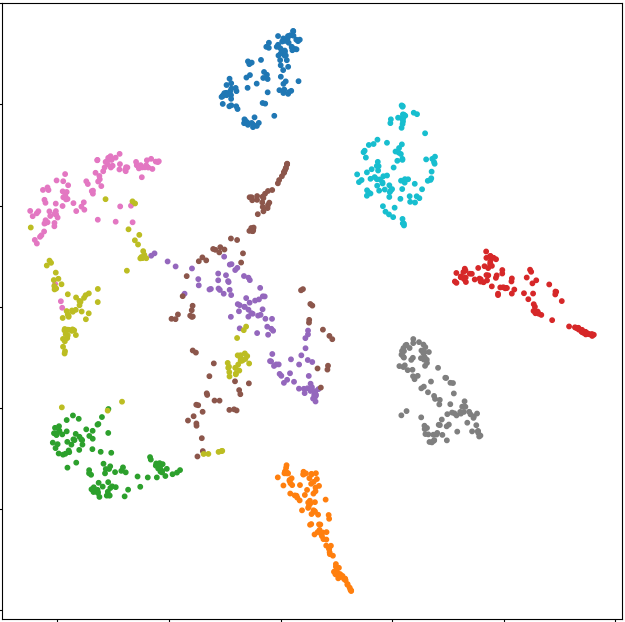
\includegraphics[width=0.26\linewidth]{simsiam_baseline.png}
        \label{simsiam_baseline_tsne}
    }
    \subfloat[]{
        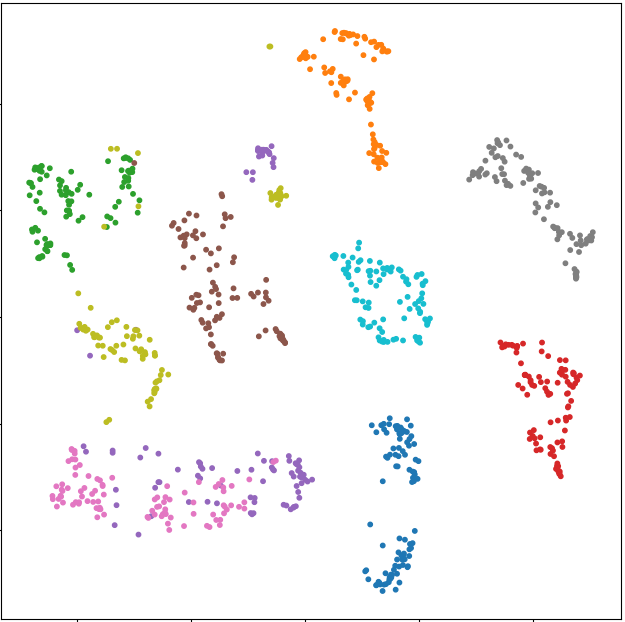
\includegraphics[width=0.26\linewidth]{simclr_baseline.png}
        \label{simclr_baseline_tsne}
    }
    \subfloat[]{
        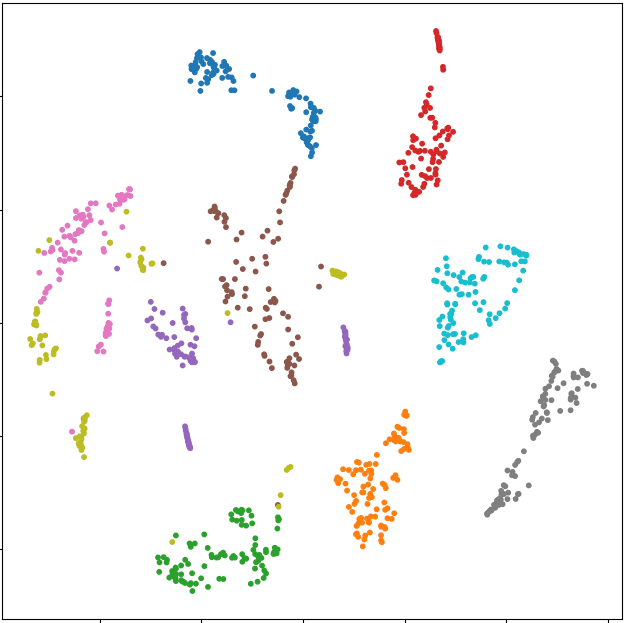
\includegraphics[width=0.26\linewidth]{byol_baseline.png}
        \label{byol_baseline_tsne}
    }
    \\
    % 第二行:MoCo、SwAV
    \subfloat[]{
        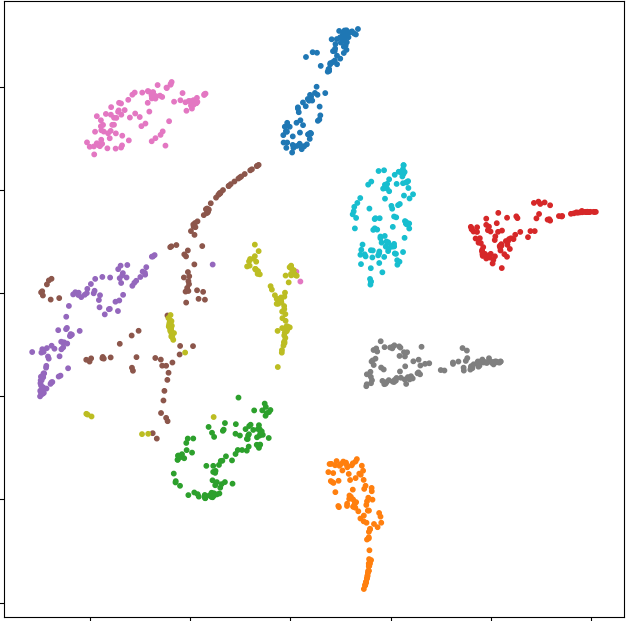
\includegraphics[width=0.26\linewidth]{moco_baseline.png}
        \label{moco_baseline_tsne}
    }
    \subfloat[]{
        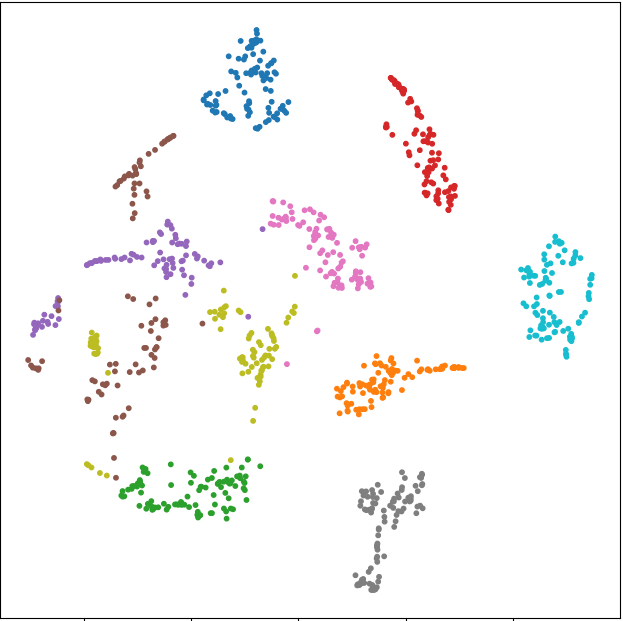
\includegraphics[width=0.26\linewidth]{swav_baseline.png}
        \label{swav_baseline_tsne}
    }
    \\
    % 第三行:SimSiam AA、SimCLR AA、BYOL AA
    \subfloat[]{
        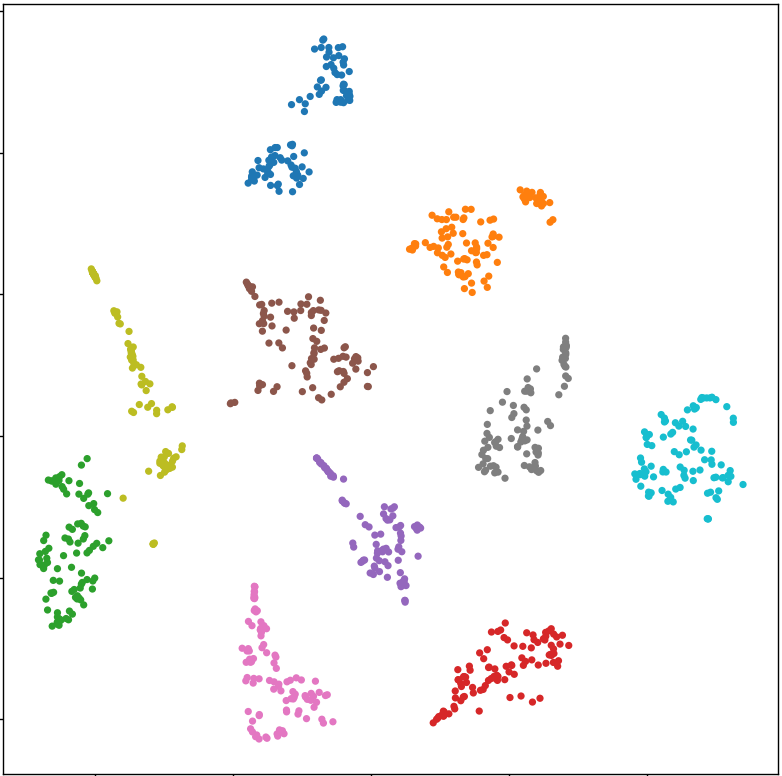
\includegraphics[width=0.26\linewidth]{simsiam_tsne.png}
        \label{simsiam_tsne}
    }
    \subfloat[]{
        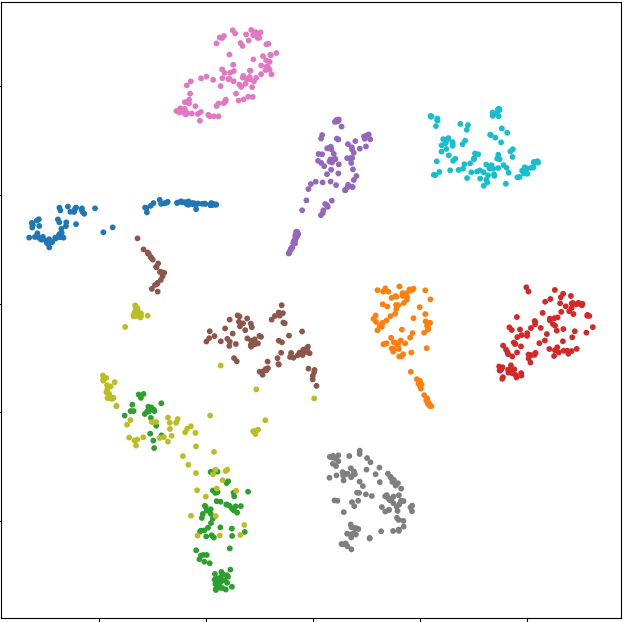
\includegraphics[width=0.26\linewidth]{simclr_batch_size_16.png}
        \label{simclr_tsne}
    }
    \subfloat[]{
        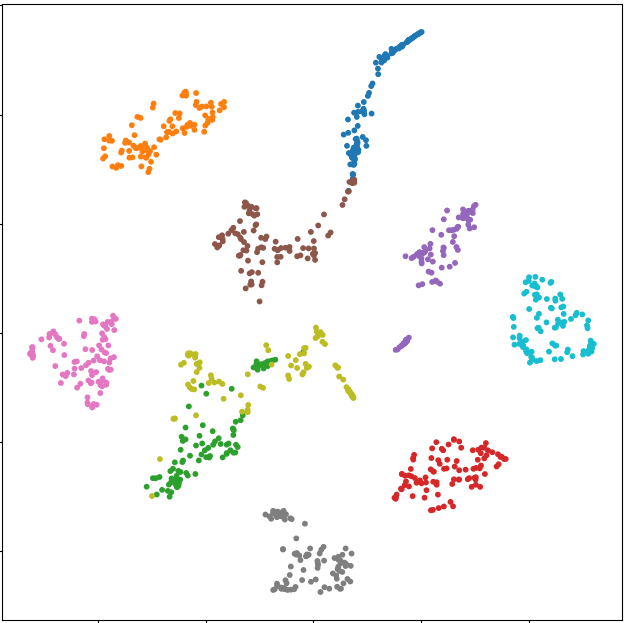
\includegraphics[width=0.26\linewidth]{byol_batch_size_128.png}
        \label{byol_tsne}
    }
    \\
    % 第四行:MoCo AA、SwAV AA、CNN、SVM
    \subfloat[]{
        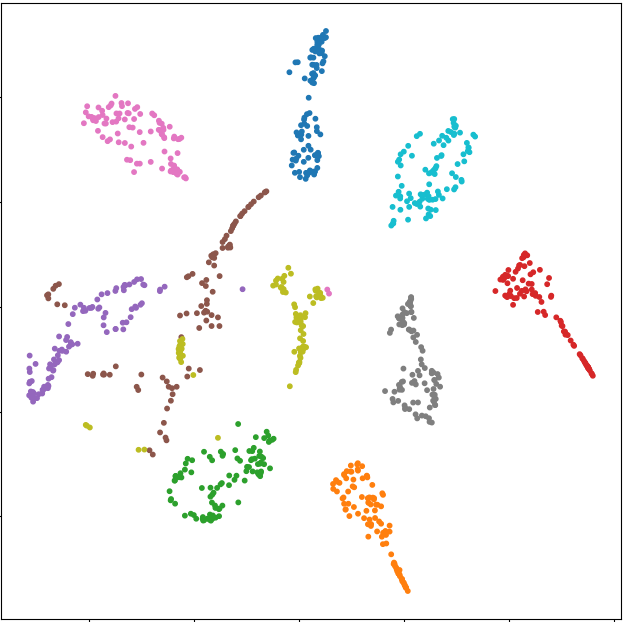
\includegraphics[width=0.26\linewidth]{moco_tsne.png}
        \label{moco_tsne}
    }
    \subfloat[]{
        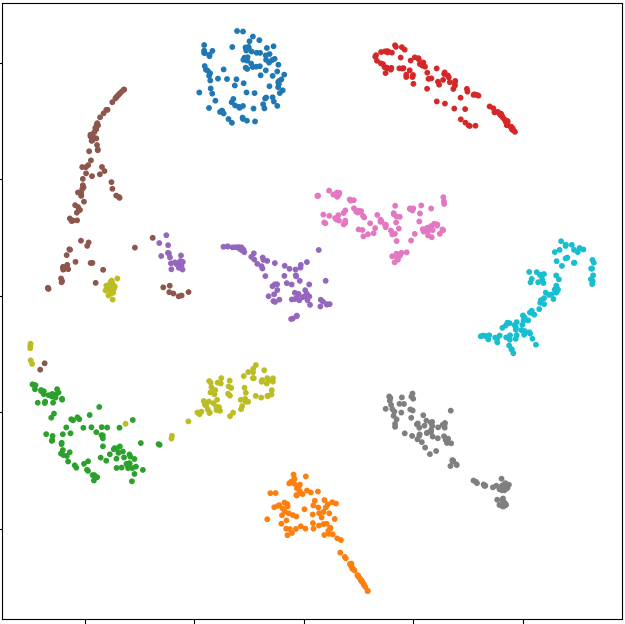
\includegraphics[width=0.26\linewidth]{swav_tsne.png}
        \label{swav_tsne}
    }
    \caption{CWRU数据集验证集数据经特征提取的 T-SNE 可视化:(a) SimSiam;(b) SimCLR;(c) BYOL;(d) MoCo;(e) SwAV;(f) SimSiam + AutoAugment;(g) SimCLR + AutoAugment;(h) BYOL + AutoAugment;(i) MoCo + AutoAugment;(j) SwAV + AutoAugment}
    \label{tsne_of_all_models}
\end{figure}

\begin{figure}[H]
    \centering
    % 第一行:SimSiam、SimCLR、BYOL(before)
    \subfloat[]{
        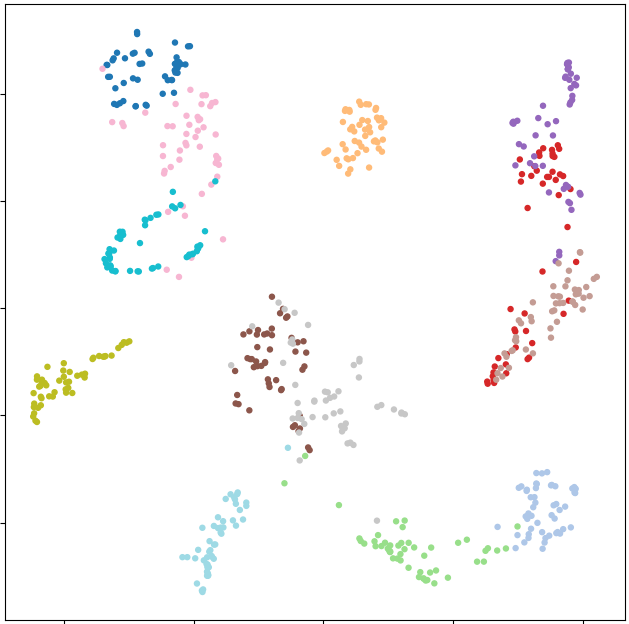
\includegraphics[width=0.26\linewidth]{simsiam_before.png}
        \label{simsiam_before_tsne}
    }
    \subfloat[]{
        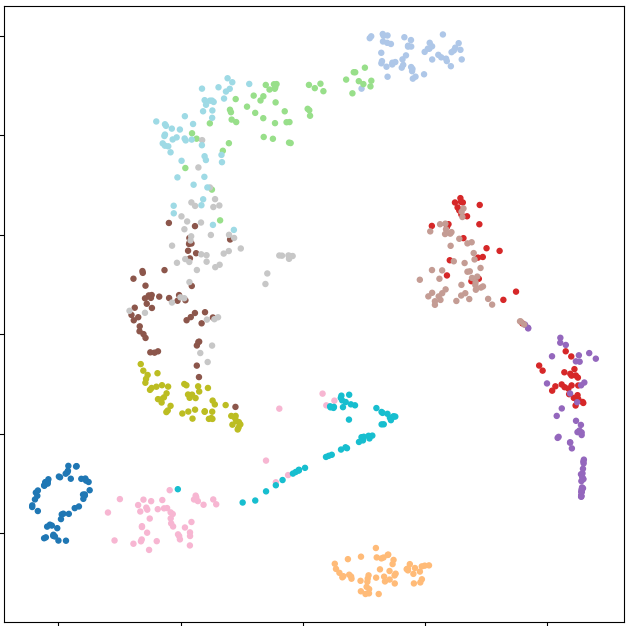
\includegraphics[width=0.26\linewidth]{simclr_before.png}
        \label{simclr_before_tsne}
    }
    \subfloat[]{
        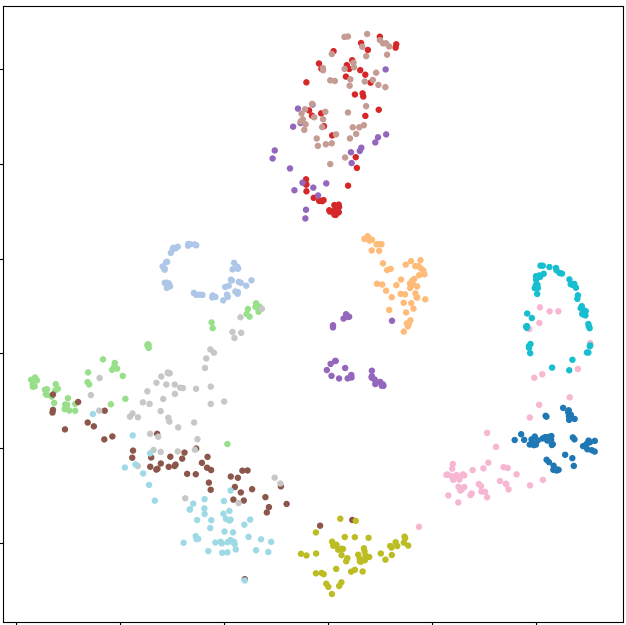
\includegraphics[width=0.26\linewidth]{byol_before.png}
        \label{byol_before_tsne}
    }
    \\
    % 第二行:MoCo、SwAV(before)
    \subfloat[]{
        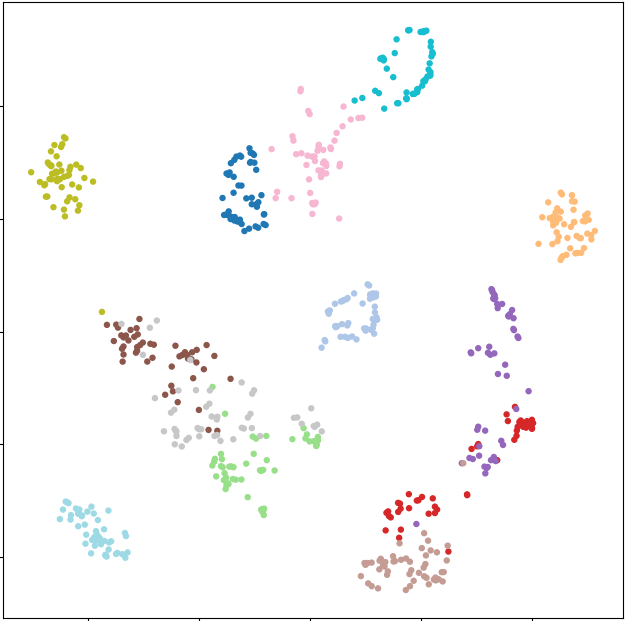
\includegraphics[width=0.26\linewidth]{moco_before.png}
        \label{moco_before_tsne}
    }
    \subfloat[]{
        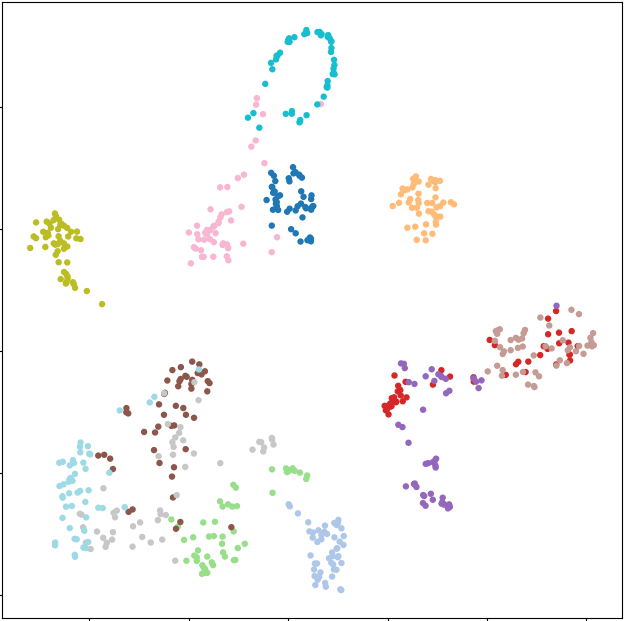
\includegraphics[width=0.26\linewidth]{swav_before.png}
        \label{swav_before_tsne}
    }
    \\
    % 第三行:SimSiam、SimCLR、BYOL(after)
    \subfloat[]{
        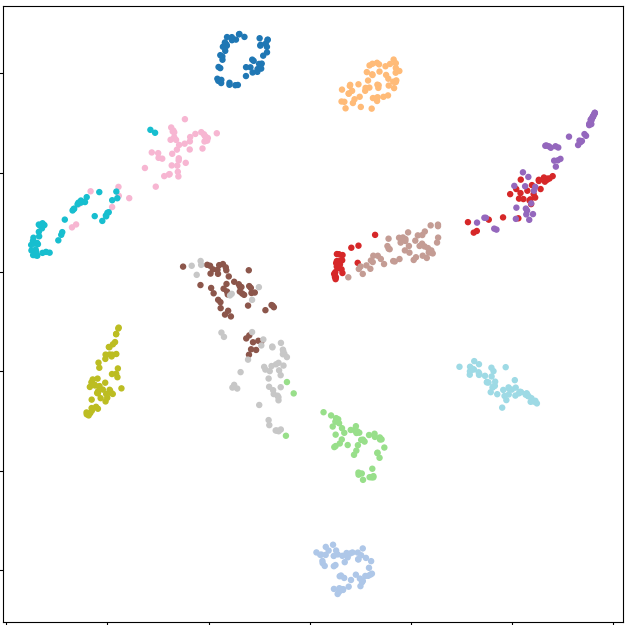
\includegraphics[width=0.26\linewidth]{simsiam_after.png}
        \label{simsiam_after_tsne}
    }
    \subfloat[]{
        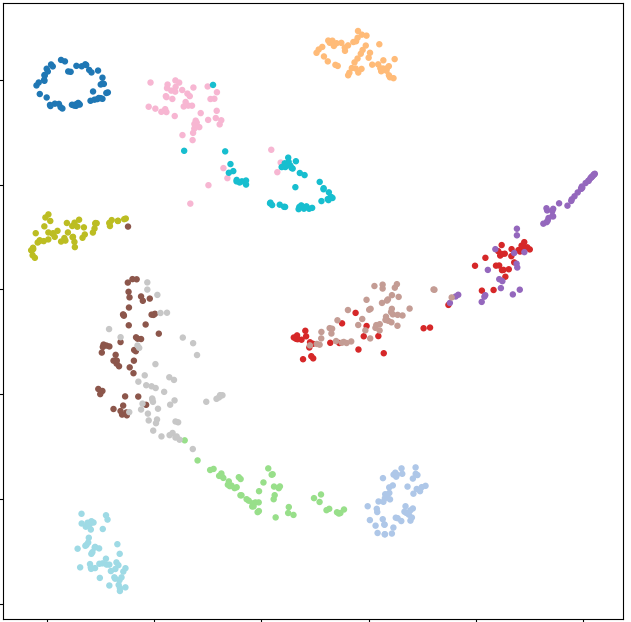
\includegraphics[width=0.26\linewidth]{simclr_after.png}
        \label{simclr_after_tsne}
    }
    \subfloat[]{
        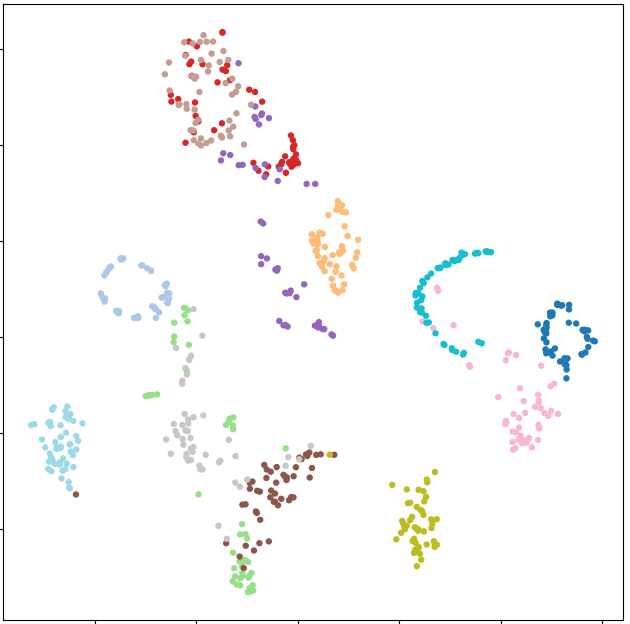
\includegraphics[width=0.26\linewidth]{byol_after.png}
        \label{byol_after_tsne}
    }
    \\
    % 第四行:MoCo、SwAV(after)
    \subfloat[]{
        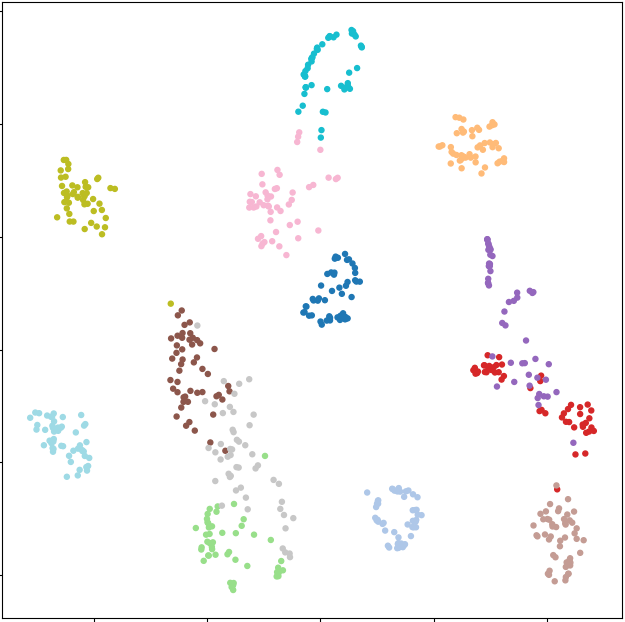
\includegraphics[width=0.26\linewidth]{moco_after.png}
        \label{moco_after_tsne}
    }
    \subfloat[]{
        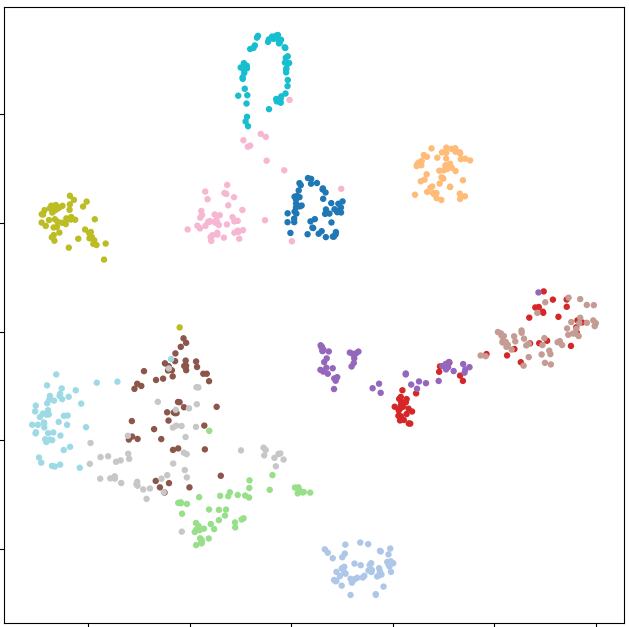
\includegraphics[width=0.26\linewidth]{swav_after.png}
        \label{swav_after_tsne}
    }
    \caption{PU数据集验证集数据经特征提取的 T-SNE 可视化:(a) SimSiam;(b) SimCLR;(c) BYOL;(d) MoCo;(e) SwAV;(f) SimSiam + AutoAugment;(g) SimCLR + AutoAugment;(h) BYOL + AutoAugment;(i) MoCo + AutoAugment;(j) SwAV + AutoAugment}
    \label{tsne_of_all_models_pu}
\end{figure}

此外,t-SNE图也揭示了不同模型对AutoAugment敏感性的差异。SimSiam和SimCLR 的表现改进较为显著,尤其在类间边界的清晰度上,它们能够较好地从增强样本中提取到更丰富的特征信息,并进一步提升了在长尾数据中的表征能力。与此相比,MoCo和SwAV的提升幅度相对有限,表明这些模型对于增强策略的依赖性较低,可能由于其结构设计本身已经能够较好地处理数据的不平衡性。

总体来看,AutoAugment 的引入在所有自监督方法中都有效提升了其在特征学习阶段的判别性能,增强了类内聚集和类间分离的能力。这种提升在两个数据集上均有体现,并与表~\ref{tab:longtail_autoaugment_comparison}和表~\ref{tab:longtail_autoaugment_comparison_pu}中的定量评估结果相一致。然而,也应注意到,特征空间可视化的改善并不总是直接转化为分类性能的提升。例如,在CWRU数据集中,尽管SimSiam的特征分布相比SimCLR更加分明,表明其在特征表示能力上有所优势,但在最终分类结果上,SimCLR仍在多个$\beta$值下表现优于SimSiam。特别是在$\beta=100$时,SimSiam的分类准确率比SimCLR低了2.44\%。这种偏差可能是由于微调阶段的分类器在训练过程中仍受到长尾数据分布带来的样本不均衡影响,导致模型更容易对高频类别过拟合,从而影响整体分类表现。这一现象表明,虽然增强策略能够显著改善特征学习阶段的表现,但对于极度不平衡的数据,如何合理调整分类器的训练过程仍是一个亟待解决的问题,在下一章我们将结合半监督学习思想和决策边距调整优化长尾分布数据在微调训练过程对模型分类器层的影响。

\FloatBarrier  % 阻止后续浮动体越过这条线

\subsection{自适应数据增强策略迁移实验结果}
在本节中,我们将探讨自适应数据增强策略的迁移实验结果,重点分析不同对比学习方法之间的迁移效果。由于从头开始训练自适应数据增强策略控制器需要较长时间,本实验旨在研究是否可以将已训练完成的控制器输出参数迁移到新的训练任务中,以节省计算资源和时间。具体而言,我们将一种对比学习方法中学到的自适应数据增强策略控制器输出参数迁移至其他对比学习方法中,评估其在不同目标模型上的迁移效果与表现。

表~\ref{tab:autoaugment_transfer_estimation}与表~\ref{tab:autoaugment_transfer_estimation_pu}展示了将某一对比学习方法中学到的自适应数据增强策略迁移至其他方法时的分类准确率表现。对角线上的数值表示各方法在使用自身策略时的性能,而非对角线上的数值则反映该方法的策略在其他目标模型中的迁移效果。总体来看,SimSiam和SimCLR学到的增强策略在CWRU和PU数据集上均展现了较强的通用性和适应性,能够在多个目标模型中迁移并保持较高的准确率,表明这些策略具有较好的跨模型重用价值。而BYOL的策略在迁移时表现较差,尤其是在PU数据集上的迁移效果较低,可能与其特有的训练机制和优化目标有关,限制了其在其他模型中的适用性。MoCo v2和SwAV的策略迁移稳定,尽管准确率有所下降,但迁移效果仍较为可接受。以下进行具体分析。

在CWRU数据集上,SimCLR和SimSiam的增强策略表现出色,分别在迁移后的准确率上达到了93.98\%和92.22\%,均为较高水平。这表明,SimCLR和SimSiam学到的增强策略具有较强的通用性,能够适应不同模型架构及数据分布。相对而言,BYOL在CWRU数据集上的迁移效果较差,其策略在迁移到其他模型时的准确率普遍低于90\%,最高为90.12\%。这表明,BYOL的增强策略可能与其特有的无负样本机制和非对称结构密切相关,使得其策略在迁移时对模型架构具有较强的依赖性,难以适应其他模型。

在PU数据集上,SimSiam和SimCLR的迁移效果依然稳定,SimSiam的策略在迁移后的准确率为82.15\%,而SimCLR的策略为82.00\%,这表明它们的增强策略能够适应PU数据集的特性。然而,BYOL在PU数据集上的表现不佳,策略迁移后的准确率仅为75.54\%,说明其增强策略对PU数据集特定数据分布的适应性较差。MoCo v2和SwAV的策略迁移效果相对稳定,尽管准确率略有下降,但仍维持在较高水平。例如,MoCo v2的迁移准确率为79.38\%,SwAV为76.62\%,这些结果表明,尽管迁移性能略逊于SimCLR和SimSiam,MoCo v2和SwAV的增强策略在多种模型架构中都能较好适应。

\begin{table}[h]
    \centering
    \caption{CWRU数据集不同对比学习方法的自适应数据增强策略学习到的控制器输出参数迁移效果准确率}
    \renewcommand\arraystretch{1.3}
    \begin{tabular}{lccccc}
        \toprule
        源策略 $\rightarrow$ 目标模型 & SimSiam & SimCLR & BYOL & MoCo v2 & SwAV \\
        \midrule
        SimSiam    & \textbf{92.08\%} & 92.22\% & 91.91\% & 92.31\% & 92.13\% \\
        SimCLR     & 92.87\% & \textbf{93.98\%} & 91.97\% & 92.43\% & 91.93\% \\
        BYOL       & 89.92\% & 89.53\% & \textbf{89.04\%} & 89.62\% & 90.12\% \\
        MoCo v2    & 91.23\% & 91.63\% & 90.88\% & \textbf{92.81\%} & 92.43\% \\
        SwAV       & 90.83\% & 92.03\% & 90.72\% & 91.92\% & \textbf{92.60\%} \\
        \bottomrule
    \end{tabular}
    \label{tab:autoaugment_transfer_estimation}
\end{table}

综上所述,SimSiam和SimCLR的增强策略在不同数据集和对比学习模型中展现了较强的迁移适应性,而BYOL的策略在迁移时的效果相对较差,尤其是在PU数据集上的迁移表现较为低下。MoCo v2和SwAV的策略迁移效果稳定,尽管准确率有所下降,但在跨模型迁移时依然保持了较高的性能。这些实验结果验证了自适应数据增强策略在不同模型和数据集间的迁移能力,为未来构建具有更强迁移适应性的增强方法提供了实证依据,同时也为开发更加通用和模块化的数据增强方法奠定了基础。

\begin{table}[h]
    \centering
    \caption{PU数据集不同对比学习方法的自适应数据增强策略学习到的控制器输出参数迁移效果准确率}
    \renewcommand\arraystretch{1.3}
    \begin{tabular}{lccccc}
        \toprule
        源模型 $\rightarrow$ 目标模型 & SimSiam & SimCLR & BYOL & MoCo v2 & SwAV \\
        \midrule
        SimSiam    & \textbf{82.15\%} & 81.84\% & 78.52\% & 79.55\% & 78.24\% \\
        SimCLR     & 81.34\% & \textbf{82.00\%} & 78.98\% & 80.31\% & 79.15\% \\
        BYOL       & 76.13\% & 76.22\% & \textbf{75.54\%} & 75.24\% & 76.48\% \\
        MoCo v2    & 79.55\% & 79.15\% & 77.46\% & \textbf{79.38\%} & 78.26\% \\
        SwAV       & 77.04\% & 77.53\% & 75.12\% & 76.68\% & \textbf{76.62\%} \\
        \bottomrule
    \end{tabular}
    \label{tab:autoaugment_transfer_estimation_pu}
\end{table}

\subsection{消融实验}
本节基于CWRU与PU两个滚动轴承故障诊断数据集,系统分析了AutoAugment中各数据增强子策略的具体作用。通过对比表~\ref{tb:da_discuss_results}与表~\ref{tb:da_discuss_results_pu}中不同数据增强子策略移除后模型在不同超参数$\beta$值下的性能变化,并结合图~\ref{train_process_da_discuss}所示训练过程中损失函数与特征标准差的演化过程,深入探讨了各策略对模型稳定性与泛化能力的影响。

实验结果表明,缩放操作对模型性能的提升最为显著。在表格3-7中,移除缩放操作(DA4)后,模型在CWRU数据集上的平均准确率下降至0.8127,较Baseline下降0.0998,是所有子策略中性能下降幅度最大的;表格3-8中,PU数据集上的平均准确率亦下降至0.7239,下降幅度为0.0344。缩放增强模拟了振动信号在幅值与尺度上的变化,使模型能够捕捉多尺度特征,提升对运行状态差异的识别能力,其缺失导致模型对幅度变异信号的适应能力明显削弱,泛化性能受限。

块打乱与掩码策略在两个数据集中亦表现出稳定的性能贡献。在CWRU数据中,移除块打乱(DA3)与掩码(DA0)后的平均准确率分别为0.8541与0.8759,性能下降幅度分别为0.0584与0.0366;而在PU数据集上,相应准确率分别为0.7357与0.7530,下降0.0226与0.0053。这类策略通过引入局部扰动与信息缺失,强化了模型在时序结构不连续或局部遮挡情形下的特征感知能力。块打乱扰乱了信号的连续性,引导模型学习局部模式;掩码则引入局部空洞,迫使模型从残缺信息中提取完整语义,增强鲁棒性。

相比之下,高斯噪声与相位扰动对模型性能的影响相对温和。CWRU数据中,移除高斯噪声(DA1)与相位扰动(DA2)后准确率分别下降至0.8756与0.8444,变化幅度为0.0369与0.0681;PU数据中准确率分别为0.7484与0.7340,下降0.0099与0.0243。这类增强通过微弱扰动模拟实际工况下的传感器噪声或频域偏移,虽能增加样本多样性,但其生成数据与原始信号相似度较高,未能显著增强模型对复杂分布的适应能力。

\begin{table}[H]
    \caption{CWRU数据集移除不同数据增强子策略在不同 $\beta$ 值下的准确率/宏平均召回率,以及相比于Baseline的变化(以SimSiam为例),移除的数据增强子策略按编号顺序为掩码、高斯噪声、相位扰动、块打乱、缩放、绝对值、竖直翻转、水平翻转}
    \centering
    \begin{tabular}{ccccccccc}
    \toprule
    $\beta$  & DA0 & DA1 & DA2 & DA3 & DA4 & DA5 & DA6 & DA7 \\
    \midrule
    1   & 0.9279  & 0.9127 & 0.9254 & 0.9204 & 0.9106 & 0.9298 & 0.9394 & 0.9338  \\
    10  & 0.9258  & 0.9348 & 0.8944 & 0.9298 & 0.8792 & 0.9358 & 0.9333 & 0.9442  \\
    50  & 0.8563  & 0.8379 & 0.8221 & 0.8467 & 0.7490 & 0.8165 & 0.8573 & 0.8387  \\
    100 & 0.7935  & 0.8169 & 0.7356 & 0.7194 & 0.7119 & 0.7912 & 0.8333 & 0.7869  \\
    \midrule
    平均值 & 0.8759 & 0.8756 & 0.8444 & 0.8541 & 0.8127 & 0.8683 & 0.8908 & 0.8759 \\
    \midrule
    变化 & -0.0366 & -0.0369 & -0.0681 & -0.0584 & \textbf{-0.0998} & -0.0442 & -0.0217 & -0.0366 \\
    \bottomrule
    \end{tabular}
    \label{tb:da_discuss_results}
\end{table}

\begin{table}[H]
\caption{PU数据集移除不同数据增强子策略在不同 $\beta$ 值下的准确率,以及相比于Baseline的变化(以SimSiam为例),移除的数据增强子策略按编号顺序为掩码、高斯噪声、相位扰动、块打乱、缩放、绝对值、竖直翻转、水平翻转}
\centering
\begin{tabular}{ccccccccc}
\toprule
$\beta$ & DA0 & DA1 & DA2 & DA3 & DA4 & DA5 & DA6 & DA7 \\
\midrule
1 & 0.8196 & 0.8202 & 0.7902 & 0.8025 & 0.7808 & 0.7932 & 0.8104 & 0.8085 \\
10 & 0.7914 & 0.7804 & 0.7794 & 0.7734 & 0.7695 & 0.7844 & 0.7876 & 0.7814 \\
50 & 0.7052 & 0.6986 & 0.6952 & 0.6965 & 0.6844 & 0.6968 & 0.7074 & 0.7052 \\
100 & 0.6958 & 0.6944 & 0.6712 & 0.6704 & 0.6608 & 0.6856 & 0.6915 & 0.6888 \\
\midrule
平均值 & 0.7530 & 0.7484 & 0.7340 & 0.7357 & 0.7239 & 0.7400 & 0.7492 & 0.7460 \\
\midrule
变化 & -0.0053 & -0.0099 & -0.0243 & -0.0226 & -0.0344 & -0.0183 & -0.0091 & -0.0123 \\
\bottomrule
\end{tabular}
\label{tb:da_discuss_results_pu}
\end{table}

绝对值操作对模型性能亦有一定促进作用。在CWRU数据中移除此策略(DA5)后,模型平均准确率下降至0.8683,下降幅度为0.0442;在PU数据中为0.7400,下降0.0183。该策略通过将信号中的负值映射为正值,引入了对称性变化,使模型在处理具有周期性或镜像对称性的信号时更具稳健性,同时在一定程度上缓解了表征空间坍塌现象。

竖直翻转与水平翻转策略对性能的影响最小。在CWRU数据集中,移除竖直翻转(DA6)与水平翻转(DA7)后模型准确率分别为0.8908与0.8759,变化幅度为0.0217与0.0366;PU数据集中分别为0.7492与0.7460,下降幅度为0.0091与0.0123。这类空间排列变换未显著改变信号的频谱特征,对于具有周期性结构的振动信号而言,其增强效果相对有限。

为了进一步理解各增强策略在训练动态中的作用及其对表征分布的影响,训练过程的演化曲线亦被纳入分析。图~\ref{train_process_da_discuss:std}进一步展示了移除不同数据增强子策略后模型训练过程中的损失函数与特征标准差变化曲线。在所有实验中,模型最终均收敛于稳定水平,特征标准差收敛值约为$1/\sqrt{d} \approx 0.625$,说明即便在缺失个别增强策略的情况下,对比学习网络仍能维持分布控制能力。然而在缩放与块打乱移除的情形下,训练曲线波动明显,收敛速度变慢,表明这些策略对模型训练过程的稳定性起到了关键作用。

综上所述,缩放操作是最具影响力的增强策略,其次为块打乱与掩码操作;高斯噪声、相位扰动及绝对值操作提供了中等增益;竖直与水平翻转的贡献最小。合理组合上述增强策略不仅能够丰富输入数据的表达形式,还能有效引导孪生网络学习更具判别力与泛化能力的特征表示,为滚动轴承的无监督故障诊断提供坚实基础。
\begin{figure}[H]
    \centering
    \subfloat[]{
        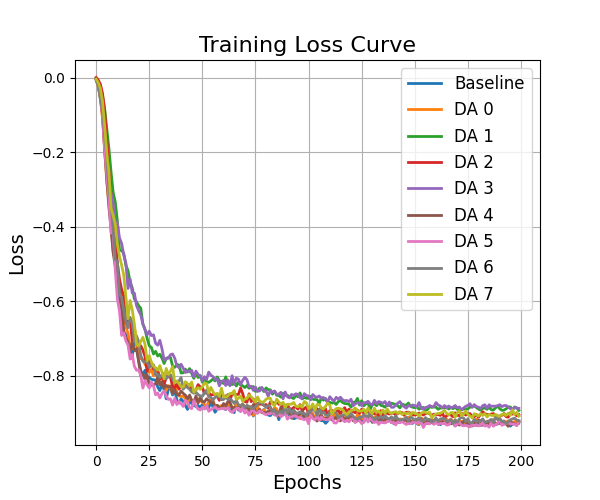
\includegraphics[width=0.45\linewidth]{loss_da.png}
        \label{train_process_da_discuss:loss}
    }
    \subfloat[]{
        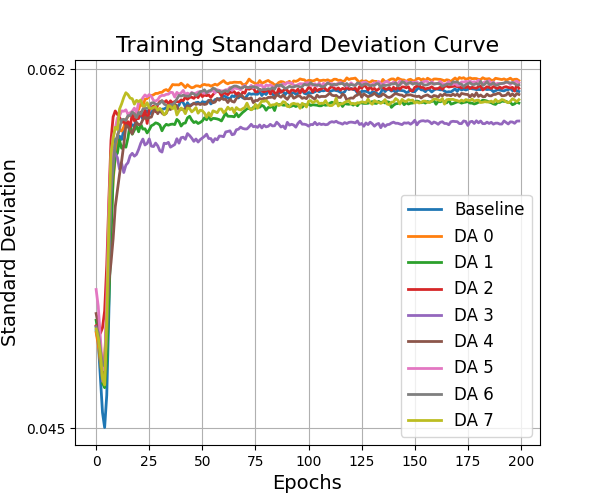
\includegraphics[width=0.45\linewidth]{std_da.png}
        \label{train_process_da_discuss:std}
    }
    \caption{移除不同数据增强子策略的训练过程对比,移除的数据增强子策略按编号顺序为掩码、高斯噪声、相位扰动、块打乱、缩放、绝对值、竖直翻转、水平翻转(a) 损失函数;(b) 提取特征的标准差}
    \label{train_process_da_discuss}
\end{figure}

\FloatBarrier  % 阻止后续浮动体越过这条线
\section{本章小结}
本章提出了一种自适应数据增强框架,旨在优化对比学习中传统的固定增强策略,并成功应用于构建符合帕累托长尾分布的CWRU和PU故障诊断数据集。实验结果表明,该方法在解决长尾分布问题时显著提升了模型性能,验证了其在轴承故障诊断任务中的实用性与有效性。此外,迁移实验结果表明,自适应数据增强控制器参数具有较强的迁移性,能够有效减少实际训练过程中的计算资源消耗。通过系统性的消融实验,进一步分析了不同增强子策略对模型性能的影响,揭示了自适应增强机制在提升模型泛化能力方面的关键作用。

然而实验也表明,在微调阶段,模型的分类器训练过程仍受到一定程度的长尾分布影响,造成分类偏差,主要源于样本分布不均所带来的训练偏差。为此,下一章将针对该问题,提出一种结合半监督边距调整优化的微调策略,以进一步提升模型在长尾条件下的分类性能。

\chapter{结合半监督边距调整优化的对比学习故障诊断网络}

在上一章节中,我们介绍了一种基于自适应数据增强优化的对比学习孪生故障诊断网络框架,在处理故障诊断中的长尾分布问题时表现出较好的性能。然而,在微调阶段,样本分布不均衡仍对模型性能造成一定影响,具体表现为分类器决策边界的偏移(如图~\ref{decision_edge_bias}所示):决策边界更倾向于尾部类的特征空间,导致头部类在特征空间中占据更大体积,进而影响尾部类的分类准确性。

针对这一问题,本章引入一种结合半监督学习与边距校准的微调策略,以缓解长尾分布对决策边界带来的偏移效应,并提升尾部类的识别能力。该方法基于决策边距调整机制,在微调阶段引入边距参数校准,通过训练可学习参数 $\omega$ 和 $\beta$ 对 logits 偏差进行修正,从而改善模型在类别不均衡场景下的判别能力。

文献~\cite{wang2023margin} 表明,边距调整在长尾学习任务中能够有效缓解类别不均带来的分类性能下降。然而,该方法未充分利用无标签数据,限制了其泛化能力和适应性。因此,本文在决策边距调整算法基础上引入半监督学习思想,结合伪标签机制和一致性正则化,利用未标记样本辅助模型边界校准,以增强模型在少样本类别下的判别能力。

本章提出的结合半监督边距调整的两阶段微调方法,在引入 AutoAugment 数据增强模块的基础上,旨在进一步提升长尾分布条件下的故障诊断性能。该方法特别适用于尾部类样本稀缺的轴承故障诊断环境,具有显著的优化潜力,能够有效缓解数据不平衡带来的挑战,增强模型在少数类样本上的判别能力。

\section{模型架构}

\subsection{结合半监督边距调整的两阶段式微调策略}

在完成对比学习模型的预训练后,如何在有限标注样本条件下充分挖掘未标注数据的潜在信息,是构建高鲁棒性智能诊断系统的关键。针对该问题,本文提出一种结合伪标签机制与边距调节策略的两阶段半监督微调框架(Semi-Marc),旨在进一步提升模型的判别能力与泛化性能。

该微调框架的整体流程如图~\ref{semi_Marc_simsiam}所示,主要包括两个阶段:

在第一阶段,利用经过预训练和初步微调的对比学习模型作为“基分类器”,对无标签样本进行推理并生成伪标签。随后,伪标签样本与原始有标签样本共同组成扩展训练集。在该阶段中,编码器部分保持冻结,仅对分类器进行微调,以获得适应新分布的“半监督分类器”。

在第二阶段,固定“半监督分类器”的全部参数,进一步引入边距校准模块,对分类器输出的 logits 进行后验调整。具体而言,基于伪标签样本与原始有标签样本共同组成的扩展训练集训练两个可学习的标量因子:尺度因子 $\omega$ 用于调节 logits 的幅度,偏置因子 $\beta$ 用于修正各类别间的边界偏差,以提升模型在不平衡分布下的置信度估计和分类能力。


\begin{figure}[H]
    \centering
    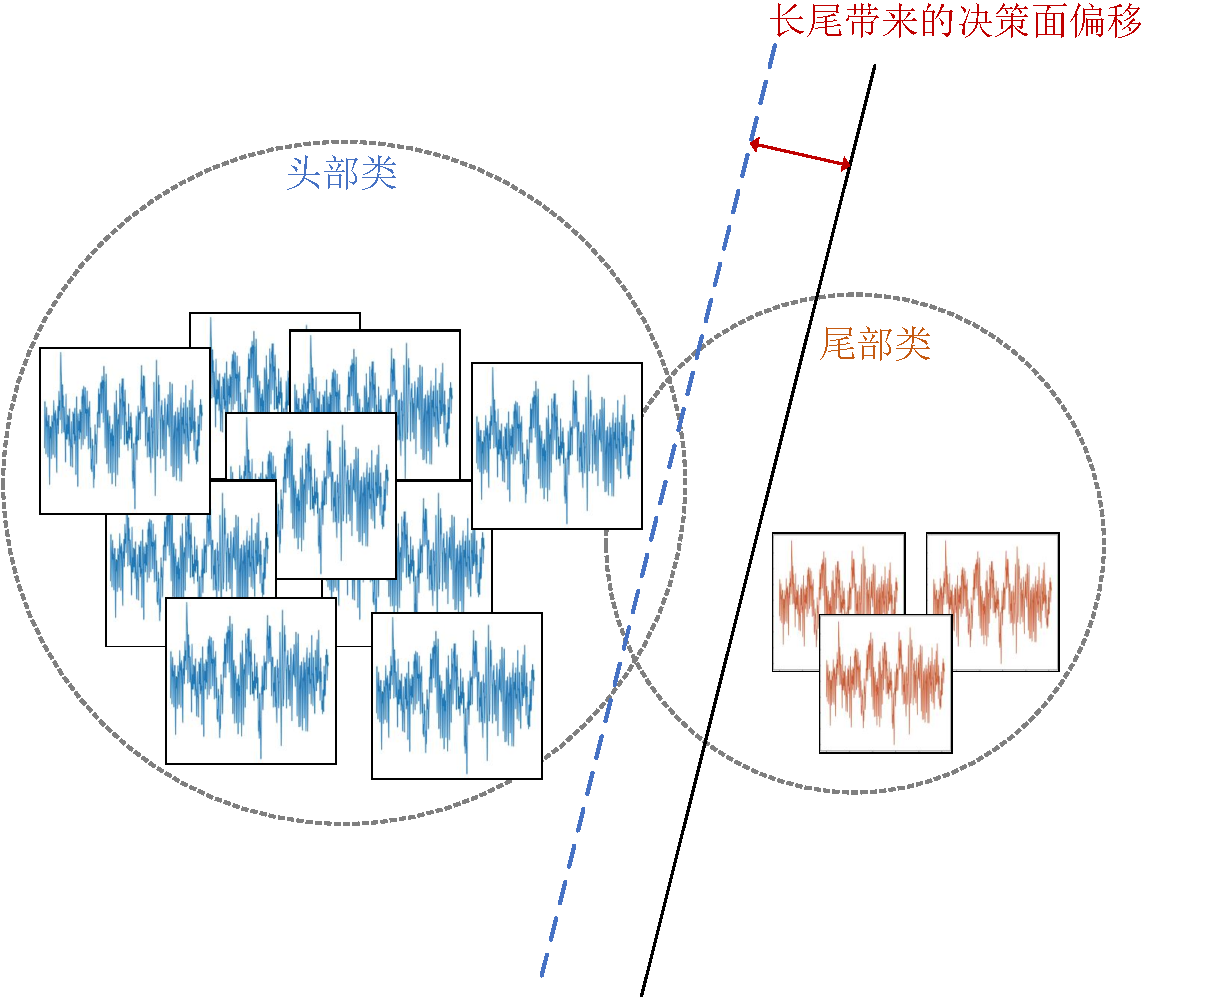
\includegraphics[width=12cm]{decision_edge_bias.pdf}
    \caption{由长尾分布带来的决策面偏移示意图}
    \label{decision_edge_bias}
\end{figure}

\begin{figure}[H]
    \centering
    \includegraphics[width=15cm]{semi_Marc_simsiam.pdf}
    \caption{结合半监督边距调整的微调策略流程框图}
    \label{semi_Marc_simsiam}
\end{figure}

该两阶段训练策略在不增加模型结构复杂度的前提下,结合了半监督伪标签扩展与边距校准的优势,有效缓解了长尾分布和标注不足带来的性能瓶颈,为轴承故障诊断场景中的少样本故障诊断任务提供了一种可行的优化路径。

\subsection{半监督学习模型架构}
本研究提出了一种结合半监督学习与决策边界调整算法的框架,以有效解决长尾分布和样本不平衡问题。受到文献\cite{yang2020rethinking,wang2023margin}的启发,研究借鉴了半监督学习(Semi-Supervised Learning)的经典流程(如图~\ref{semi_supervise_procedure}所示)。该流程分为两个阶段:

在第一阶段,使用原始的不平衡标记数据集 $\mathcal{D}_{L}$ 训练一个初步分类器 $f_{\hat{\theta}}$。随后,在第二阶段,利用该分类器对未标记数据集 $\mathcal{D}_{U}$ 进行推断并生成伪标签 $\hat{y}$。伪标签数据与标记数据结合,通过最小化以下损失函数优化模型:
\begin{equation} 
    \mathcal{L}(\mathcal{D}_{L},\theta) + \omega \mathcal{L}(\mathcal{D}_{U},\theta), 
    \label{eq:semi_loss}
\end{equation}
其中,$\omega$ 为未标记数据的损失权重,$\mathcal{L}(\mathcal{D}_{L},\theta)$ 和 $\mathcal{L}(\mathcal{D}_{U},\theta)$ 分别代表基于标记数据和伪标签数据的损失项。通过整合这两部分损失,最终得到优化后的分类器 $f_{\hat{\theta_f}}$,以更好地建模数据分布,尤其是尾部类别(少数类别)。该过程通过充分利用未标记数据 $\mathcal{D}_{U}$,提升模型对少数类别的分类能力,从而显著优化其决策边界。

\begin{figure}[h]
    \centering
    \includegraphics[width=10cm]{semi_supervise_procedure.pdf}
    \caption{半监督学习流程图}
    \label{semi_supervise_procedure}
\end{figure}

\subsection{经半监督优化的决策面调整算法}

在处理长尾分布和类别不平衡问题时,决策面调整方法被广泛认为是一种有效手段,能够显著提升模型在尾部类别上的判别能力。文献\citing{wang2023margin}提出了一种基于边距校准的决策面调整方法——Marc(Margin Calibration),通过显式调整每个类别的决策边距,改善分类器的鲁棒性与公平性。

在长尾学习任务中,模型对不同类别的决策边距(Margin)和logits存在显著偏差。图~\ref{Marc_illustration}直观展示了边距的定义。
设类别 $j$ 的仿射超平面为 $H_j \in \mathbb{R}^{p-1}$,定义为
\[
H_j: W_j z + b_j = 0,
\]
表示特征 $z$ 落在该超平面正侧时被判定为类别 $j$。令 $z_0$ 为满足 $W_j z_0 + b_j = 0$ 的点(即落在超平面 $H_j$ 上),任取特征向量 $z_1$,则其到超平面的边距 $d_j$ 计算如下:
\begin{equation}
    \begin{split}
        d_j &= \left\| \text{proj}_{W_j}(z_1 - z_0) \right\| \\
            &= \left\| \frac{W_j \cdot (z_1 - z_0)}{\|W_j\|} \right\| \\
            &= \frac{W_j \cdot z_1 - W_j \cdot z_0}{\|W_j\|} \\
            &= \frac{W_j z_1 + b_j}{\|W_j\|} \quad (\text{由于 } W_j z_0 + b_j = 0)
    \end{split}
\end{equation}
由此,logit $= W_j z_1 + b_j = \|W_j\| d_j$,即logit本质上是边距的加权形式。

Marc引入两个参数:缩放因子 $\omega$ 与 偏置项 $\beta$,用于对边距 $d_j$ 进行线性变换,得到校准后的边距 $\hat{d}_j$:
\begin{equation}
    \hat{d}_j = \omega_j \cdot d_j + \beta_j
\end{equation}

调整后的logits计算如下:
\begin{equation}
    \begin{split}
        logits_{Marc} &= \| W_j \| \cdot \hat{d}_j \\
                      &= \omega_j \cdot \|W_j\| d_j + \beta_j \cdot \|W_j\| \\
                      &= \omega_j \cdot \eta_j + \beta_j \cdot \|W_j\|,
    \end{split}
\end{equation}

其中 $\eta_j = \|W_j\| d_j$ 为原始logit。$\omega_j$ 与 $\beta_j$ 作为可学习参数,通过最小化类别平衡损失(如CB Loss)进行联合优化。
为进一步提升 Marc 算法在少样本类别上的判别性能,本文引入了半监督伪标签机制。该机制首先利用预训练的主干模型对未标注样本进行推理,并为其分配伪标签。随后,将这些带有高置信度伪标签的无标签样本与原始标注样本集合并,构建联合训练集 $\mathcal{D} = \mathcal{D}_L \cup \mathcal{D}_U$,其中 $\mathcal{D}_L$ 表示人工标注的数据集,$\mathcal{D}_U$ 则为通过模型自动生成标签的无标签样本。在此联合数据集上执行边距校准优化过程,不仅增强了模型对尾部类别的判别能力,也有效缓解了因类别分布不均而导致的决策边界偏移问题。该方法在保持整体训练稳定性的同时,实现了对尾部类别边界的自适应调整,从而进一步提升了 Marc 框架在长尾分布场景中的表现。

\begin{figure}[H]
    \centering
    \includegraphics[width=10cm]{Marc_illustration.png}
    \caption{决策面与边距示意图:红色为头部类,蓝色为尾部类}
    \label{Marc_illustration}
\end{figure}
该策略不仅增强了Marc模型的边界自适应能力,也缓解了类别间的不均衡性,特别是在弱特征或类间语义重叠场景下表现更优。

\begin{table}[h]
    \centering
    {\CJKfamily{song}
    \begin{tabular}{@{}l@{}}
    \toprule
    \textbf{Marc伪代码(使用PyTorch表示)} \\
    \midrule
    \begin{lstlisting}[basicstyle=\fontspec{Times New Roman}, frame=none]
1: 初始化边距校准参数:
    omega = torch.nn.Parameter(torch.ones(1, num_classes))
    beta = torch.nn.Parameter(torch.zeros(1, num_classes))

2: 输入:联合训练数据 x 
   (包括带标签数据 D_L 和伪标签数据 D_U)

3: with torch.no_grad():
4:     w_norm = torch.norm(model.fc.weight, dim=1)
5:     logit_before = model(x)
6:     logit_after = omega * logit_before + beta * w_norm

7: 计算损失(如CB Loss),优化 omega 和 beta。
    \end{lstlisting} \\
    \bottomrule
    \end{tabular}
    }
    \caption{{\CJKfamily{song}Marc 算法实现伪代码}}
    \label{alg:Marc}
\end{table}


\subsection{实验设置}
\textbf{模型配置}:对比学习的网络结构参数设置与上一章相同。在决策面调整过程中,将 $\omega$ 初始化为大小为 $1 \times \text{num\_classes}$ 的全 $1$ 向量,而 $\beta$ 则初始化为相同大小的全 $0$ 向量。

\textbf{优化器}:本研究使用 SGD 优化器训练模型。网络参数通过公式 (\ref{eq:SGD}) 更新。学习率初始设置为 \( 0.05 \times \frac{\text{BatchSize}}{256} \),学习率采用余弦衰减调度。余弦衰减调度的公式如式(\ref{eq:cos_decay})所示。

\textbf{损失函数}:损失函数为式(\ref{eq:semi_loss}),其中$\mathcal{L}$为交叉熵损失函数式(\ref{eq:cross_entropy}),$\omega$设为0.9。

\textbf{数据细节}:
无标签数据集的规模为类别数*100,有标签数据集为不同不平衡因子构造帕累托分布的数据,测试集为均匀分布。每个样本包含 1024 个数据点。每个阶段分别训练150个周期。
在整个训练过程中,每个输入模型的 mini-batch 大小设定为 64。
\FloatBarrier  % 阻止后续浮动体越过这条线

\section{实验与分析}

\subsection{在长尾分布的 CWRU 数据集和PU数据集上的实验结果}
在本节中,我们将探讨在长尾分布数据集上,结合自适应数据增强策略AutoAugment和Semi-Marc微调策略的应用。随着长尾分布数据集的引入,分类器的训练面临着少数类别样本稀缺和类间不平衡的问题,传统的分类方法往往受到这些因素的严重影响。为了缓解这一问题,我们在引入AutoAugment数据增强模块的基础上,进一步采用了Semi-Marc微调策略,旨在优化分类器层的训练过程,减小长尾数据分布对分类器的负面影响。实验将在CWRU数据集和PU数据集上进行,分别验证该策略在不同数据集上的表现,并与传统方法进行对比,评估其在长尾分布数据下的效果。

表~\ref{tab:longtail_Semi-Marc_comparison}和表~\ref{tab:longtail_Semi-Marc_comparison_pu}分别总结了在CWRU和PU两个数据集上,不同长尾不平衡因子 \(\beta\) 条件下,各主流对比学习方法在引入Semi-Marc策略前后的分类准确率变化。其中,\(\beta=1\) 时,数据集各类别样本数量较为均衡;随着 \(\beta\) 的增大,数据分布逐渐演变为典型的长尾形态,尾部类别的样本数量明显减少,分类任务的难度随之提升。

总体而言,引入Semi-Marc微调策略后,在两个数据集的不同样本不平衡度下均展现出一定程度的性能提升。在CWRU数据集中,平均提升至少为1.35\%,并且随着数据分布不均衡度的加剧,提升幅度逐渐增大。在PU数据集中,虽然提升幅度相对较小,但同样呈现出相似的趋势,平均提升至少为1.26\%,并且在不平衡度达到50时,提升幅度显著增加至2.53\%。这一结果表明,Semi-Marc微调策略在长尾分布数据集上有效地优化了模型性能,尤其是在高不平衡因子的情况下,其优化效果愈加明显。以下将对这些提升进行更为详细的分析。

\begin{table}[!h]
    \caption{CWRU 数据集上不同 $\beta$ 值下各方法在加入 Semi-Marc 策略前后的准确率变化}
    \centering
    \renewcommand\arraystretch{1.2}
    \begin{tabular}{ccccc}
    \toprule
    $\beta$ & 方法 & 加入 AutoAugment 后 & 加入 AutoAugment 与 Semi-Marc 后 & 提升 \\
    \midrule
    \multirow{6}{*}{1}   
        & SimSiam & 92.08\% & 94.02\% & +1.94\% \\
        & SimCLR  & 93.98\% & 95.50\% & +1.52\% \\
        & BYOL    & 89.03\% & 89.83\% & +0.80\% \\
        & MoCo v2 & 92.79\% & 94.02\% & +1.23\% \\
        & SwAV    & 92.59\% & 93.85\% & +1.26\% \\
        & 平均提升    & - & - & +1.35\% \\
    \midrule
    \multirow{6}{*}{10}  
        & SimSiam & 94.23\% & 96.24\% & +2.01\% \\
        & SimCLR  & 94.58\% & 95.82\% & +1.24\% \\
        & BYOL    & 89.42\% & 90.13\% & +0.71\% \\
        & MoCo v2 & 82.92\% & 90.26\% & +2.04\% \\
        & SwAV    & 93.53\% & 94.51\% & +0.98\% \\
        & 平均提升    & - & - & +1.40\% \\
    \midrule
    \multirow{6}{*}{50}  
        & SimSiam & 91.31\% & 92.73\% & +1.42\% \\
        & SimCLR  & 91.97\% & 94.12\% & +2.15\% \\
        & BYOL    & 84.79\% & 88.24\% & +3.45\% \\
        & MoCo v2 & 82.91\% & 85.07\% & +3.16\% \\
        & SwAV    & 82.39\% & 84.14\% & +2.75\% \\
        & 平均提升    & - & - & +2.59\% \\
    \midrule
    \multirow{6}{*}{100} 
        & SimSiam & 87.60\% & 91.45\% & +3.85\% \\
        & SimCLR  & 90.04\% & 93.02\% & +2.98\% \\
        & BYOL    & 81.12\% & 83.14\% & +2.02\% \\
        & MoCo v2 & 83.75\% & 84.35\% & +0.60\% \\
        & SwAV    & 82.40\% & 84.06\% & +1.66\% \\
        & 平均提升    & - & - & +2.22\% \\
    \bottomrule
    \end{tabular}
    \label{tab:longtail_Semi-Marc_comparison}
\end{table}

在样本数量分布较为平衡的情况下,Semi-Marc已展现出显著的性能提升效果。例如,在CWRU数据集上,SimSiam的准确率从92.08\%提升至94.02\%,提升幅度为1.94\%。这表明,即便在数据样本分布较为均衡的场景下,Semi-Marc依然能通过伪标签生成和边界调节机制,挖掘数据潜力,进而增强模型的判别能力与泛化性能。同时,SimCLR、MoCo v2和SwAV等方法也展现出不同程度的提升,进一步验证了该策略的广泛适用性。

\begin{table}[!h]
    \caption{PU 数据集上不同 $\beta$ 值下各方法在加入 Semi-Marc 策略前后的准确率变化}
    \centering
    \renewcommand\arraystretch{1.2}
    \begin{tabular}{ccccc}
    \toprule
    $\beta$ & 方法 & 加入 AutoAugment 后 & 加入 AutoAugment 与 Semi-Marc 后 & 提升 \\
    \midrule
    \multirow{6}{*}{1}   
        & SimSiam & 82.15\% & 84.04\% & +1.89\% \\
        & SimCLR  & 82.00\% & 84.32\% & +2.32\% \\
        & BYOL    & 75.54\% & 76.86\% & +1.32\% \\
        & MoCo v2 & 79.38\% & 81.07\% & +1.69\% \\
        & SwAV    & 76.62\% & 77.86\% & +1.24\% \\
        & 平均提升    & - & - & +1.35\% \\
    \midrule
    \multirow{6}{*}{10}  
        & SimSiam & 79.54\% & 81.60\% & +2.06\% \\
        & SimCLR  & 79.38\% & 80.62\% & +1.24\% \\
        & BYOL    & 74.38\% & 75.32\% & +0.94\% \\
        & MoCo v2 & 76.15\% & 77.49\% & +1.34\% \\
        & SwAV    & 73.69\% & 74.41\% & +0.72\% \\
        & 平均提升    & - & - & +1.35\% \\
    \midrule
    \multirow{6}{*}{50}  
        & SimSiam & 71.54\% & 74.96\% & +3.42\% \\
        & SimCLR  & 73.00\% & 76.15\% & +3.15\% \\
        & BYOL    & 63.92\% & 65.06\% & +1.14\% \\
        & MoCo v2 & 74.00\% & 75.42\% & +1.42\% \\
        & SwAV    & 72.92\% & 76.46\% & +3.54\% \\
        & 平均提升    & - & - & +1.35\% \\
    \midrule
    \multirow{6}{*}{100} 
        & SimSiam & 70.08\% & 72.52\% & +2.44\% \\
        & SimCLR  & 70.77\% & 72.65\% & +1.88\% \\
        & BYOL    & 59.08\% & 60.40\% & +1.32\% \\
        & MoCo v2 & 67.08\% & 68.48\% & +1.40\% \\
        & SwAV    & 66.62\% & 67.48\% & +0.86\% \\
        & 平均提升    & - & - & +1.35\% \\
    \bottomrule
    \end{tabular}
    \label{tab:longtail_Semi-Marc_comparison_pu}
\end{table}

随着 \(\beta\) 的持续增大,代表数据分布逐步偏向长尾,尾部类别样本数量显著减少,模型面临更为严峻的少数类学习挑战。此时,Semi-Marc的性能增益更加明显,尤其在极端长尾条件下,SimSiam准确率提升高达3.85\%,SimCLR也提升近3\%,BYOL在该阶段的提升达到2.02\%。这充分体现了Semi-Marc对尾部类别识别和表征能力的显著促进作用,能够有效缓解长尾数据导致的类别不平衡问题。

值得关注的是,MoCo v2与SwAV在中等不平衡条件下取得了最大性能提升。MoCo v2准确率从82.91\%上升到90.07\%,提升达到7.16\%;SwAV也有6.75\%的显著提升,表明Semi-Marc与基于字典和聚类机制的方法存在良好协同效应,显著改善尾部类别的表示能力。

BYOL的表现呈现出一定的阶段性特征。在均衡及轻度不平衡条件时,提升幅度较小,分别为0.80\%和0.71\%,但在中度和严重不平衡条件下,提升分别达到3.45\%和2.02\%,显示其在尾部类别样本稀缺时更依赖Semi-Marc所带来的边界调节机制,以提升少数类的学习能力。

SimCLR的性能提升在所有 \(\beta\) 条件下均维持在1.24\%至2.98\%之间,表现较为稳定。SimSiam虽然在均衡及轻度不平衡条件下表现优异,但在中度不平衡时提升幅度有所下降至1.42\%,表明其对尾部类别的建模能力存在一定局限,但在极端条件下仍具有较强恢复能力。

PU数据集上的实验结果与CWRU数据集表现高度一致,验证了Semi-Marc在不同数据分布和应用场景下的通用性和有效性。均衡分布下,SimSiam准确率提升1.89\%,SimCLR和BYOL也分别提升2.32\%和1.32\%。随着 \(\beta\) 增大至50,SwAV和SimSiam的提升分别达到3.54\%和3.42\%,表明在严重长尾分布中,Semi-Marc对尾部类别的表征提升尤为显著。即使在极端长尾条件下,所有方法依然保持稳定的提升幅度,表现出良好的鲁棒性。

综上所述,Semi-Marc作为一种通用且高效的半监督微调策略,在多种主流对比学习框架如SimSiam、SimCLR、BYOL、MoCo v2与SwAV下均能显著提升故障诊断准确率。其在处理长尾分布数据时表现尤为突出,能够有效缓解尾部类别样本稀缺所带来的识别困难,展现出优异的稳定性和适应能力,为轴承故障诊断领域中长尾不平衡问题提供了切实可行的解决方案。

在整体准确率提升的基础上,为了更深入地理解Semi-Marc在不同类别,尤其是尾部少数类上的表现,我们进一步分析了长尾分布数据集上各类别的分类准确率变化情况。通过对比各类别的识别效果,可以直观地观察到Semi-Marc对尾部类别样本的增强作用及其在缓解类别不平衡问题上的具体贡献。以下内容将详细展示该分析结果。



\subsection{长尾分布的数据集上训练时的各类别准确率变化}
在长尾分布数据集上,类别间的样本数量差异往往导致模型对尾部少数类的识别能力较弱。为了更好地理解Semi-Marc微调策略在长尾数据中的表现,本节将重点分析在引入该策略后,各个类别的分类准确率变化,特别是对尾部类别的影响。

从图~\ref{fig:semi_Marc_class_acc_for_beta}中可以观察到,在引入Semi-Marc微调策略后,尾部类别(如Class8)的分类准确率显著提升,表明该方法在改善模型对尾部类别判别能力方面表现出色。值得注意的是,虽然Semi-Marc的核心优化目标主要针对少样本类的边界判别力,但从图中结果来看,其对头部类与中部类的分类表现也具有一定的促进作用,这一现象在图~\ref{fig:semi_Marc_class_acc_for_beta10}、图~\ref{fig:semi_Marc_class_acc_for_beta50}和图~\ref{fig:semi_Marc_class_acc_for_beta100}中表现得尤为明显。

具体而言,在 \(\beta=10\) 的轻度不平衡设置下,尾部类别的准确率首先获得了较为温和但稳定的提升,表明伪标签和边距调整机制已初步建立对尾类的有效补偿机制。而在 \(\beta=50\) 与 \(\beta=100\) 的高度不平衡条件下,尾部类别的准确率提升幅度更为显著,说明Semi-Marc能够根据类别分布适应性地调节判别边界,在数据倾斜较严重的场景下同样保持良好的泛化能力。

值得一提的是,在绝大多数类别上引入Semi-Marc并未导致分类性能的下降。相反,头部类与中部类的准确率在一定程度上也有所提升。这可能得益于联合训练集 \(D = D_L \cup D_U\) 的构建机制在维持原始分布结构的同时,通过增加边缘样本提升了整体决策边界的清晰度,从而在全局范围内优化了类间隔。尤其是在中部类别上,这种正向迁移效应更为明显,表现为整体准确率的连续增长。

\begin{figure}[h]
    \centering
    \subfloat[]{
        \includegraphics[width=0.47\linewidth]{class_acc_for_beta=1_10avg.png}
        \label{fig:semi_Marc_class_acc_for_beta1}
    }
    \subfloat[]{
        \includegraphics[width=0.47\linewidth]{class_acc_for_beta=10.png}
        \label{fig:semi_Marc_class_acc_for_beta10}
    }
    \par\medskip
    \subfloat[]{
        \includegraphics[width=0.47\linewidth]{class_acc_for_beta=50.png}
        \label{fig:semi_Marc_class_acc_for_beta50}
    }
    \subfloat[]{
        \includegraphics[width=0.47\linewidth]{class_acc_for_beta=100.png}
        \label{fig:semi_Marc_class_acc_for_beta100}
    }
    \caption{不同$\beta$值下基于Semi-Marc微调的各类别准确率/宏平均召回率的变化(以SimSiam为例) (a) $\beta=1$;(b) $\beta=10$;(c) $\beta=50$;(d) $\beta=100$}
    \label{fig:semi_Marc_class_acc_for_beta}
\end{figure}

此外,Semi-Marc在保持编码器冻结的基础上,仅对分类器进行微调,并引入决策边界调节机制,有效缓解了类别间边界模糊的问题,从而进一步提升了模型的分类性能。该策略无需依赖复杂的数据增强操作,具备较低的计算开销与实现复杂度,仅需冻结特征提取层并对顶部分类器进行轻量级训练,因此在实际应用中具有良好的部署灵活性与扩展性,尤其适用于数据获取成本高、类别分布严重不均的故障诊断任务。

Semi-Marc作为一种轻量级的自监督模型优化方案,既提升了模型对无标签数据的利用效率,又显著增强了在尾部类别上的判别能力。图~\ref{fig:semi_Marc_class_acc_for_beta}系列进一步展示了其在多种不平衡强度下对各类别分类性能的改善趋势,尤其在尾部类上表现突出,同时也兼顾了头部与中部类别的性能稳定性,展现出良好的模型适应性与任务通用性。上述发现不仅验证了Semi-Marc在长尾场景下的有效性,也为后续提升对比学习模型在应用中的实用性与鲁棒性提供了新的研究方向。


\subsection{消融实验}
在本小节中,基于CWRU数据集和PU数据集对本章提出的模型进行了消融实验。图\ref{fig:all_models_before_after_SemiMarc}和图~\ref{fig:all_models_before_after_SemiMarc_pu}分别展示了五种主流对比学习方法(SimSiam、SimCLR、BYOL、MoCo v2和SwAV)在CWRU和PU两个数据集上,采用不同微调策略下的分类准确率表现。主要结论如下:

首先,在基础数据增强策略AutoAugment的条件下,CWRU数据集上的五种模型准确率均处于较高水平,平均约为92.13\%;而PU数据集准确率相对较低,平均约为79.14\%,反映了两个数据集在任务难度和数据分布上的差异。

引入半监督策略后,两个数据集所有模型均实现了明显的性能提升。CWRU数据集平均准确率提升至约95.46\%,提升幅度显著,表明充分利用未标注数据有助于模型捕获更丰富的特征信息,增强泛化能力。PU数据集准确率也从约79.14\%提升至约80.32\%,表现出良好的增益,尤其对任务难度较高的PU数据集意义重大。

单独采用决策边距调整策略时,两个数据集的模型表现同样有所提升。CWRU数据集平均准确率约为93.64\%,PU数据集约为79.93\%。虽然提升幅度略逊于半监督策略,但仍体现了通过调整模型决策边界增强分类判别力的有效性。

当半监督学习与决策边距调整策略结合使用时,两个数据集的模型准确率均达到最高水平。CWRU数据集平均准确率达到约95.82\%,PU数据集也提升至约80.83\%,显示两种策略在提升模型性能上具有良好互补性。尤其是在复杂工况和数据稀缺的情况下,联合策略显著促进了模型对故障特征的深度挖掘和判别能力。

\begin{figure}[H]
    \centering
    \includegraphics[width=15cm]{all_models_before_after_semimarc_pu.png}
    \caption{CWRU数据集五种主流对比学习方法在不同微调策略(仅 AutoAugment,AutoAugment+半监督,AutoAugment+决策边距调整,AutoAugment+半监督结合决策边距调整)下的分类准确率对比}
    \label{fig:all_models_before_after_SemiMarc}
\end{figure}

\begin{figure}[H]
    \centering
    \includegraphics[width=15cm]{all_models_before_after_semimarc.png}
    \caption{PU数据集五种主流对比学习方法在不同微调策略(仅 AutoAugment,AutoAugment+半监督,AutoAugment+决策边距调整,AutoAugment+半监督结合决策边距调整)下的分类准确率对比}
    \label{fig:all_models_before_after_SemiMarc_pu}
\end{figure}


综上所述,基于两类不同难度数据集的实验结果验证了多策略集成微调方法的有效性。半监督学习在提升模型泛化性上贡献最大,而决策边距调整策略则优化了分类边界。两者结合实现了对比学习模型在故障诊断任务中的显著性能提升,体现了该方法在实际应用中的广阔前景。

为了更深入理解无标签数据规模对模型性能的影响,本节进一步分析了不同规模的无监督数据在Semi-Marc微调框架下对五种主流对比学习方法分类准确率的影响。通过系统调整无标签数据数量,揭示了数据量变化对模型泛化能力和判别能力的具体作用,为后续实际应用中无标签数据的合理利用提供指导。

图~\ref{acc_vs_ssvsize_semimarc}展示了五种对比学习方法(SimSiam、SimCLR、BYOL、MoCo v2和SwAV)在不同无标签数据规模下的分类准确率变化趋势,旨在探讨数据量对模型性能的影响。

\begin{figure}[H]
    \centering
    \includegraphics[width=12cm]{acc_vs_ssvsize_semimarc.png}
    \caption{不同无标签数据集规模和不平衡因子$\beta$配置下的Semi-Marc平均准确率/宏平均召回率折线图}
    \label{acc_vs_ssvsize_semimarc}
\end{figure}


在采用Semi-Marc微调策略的设定下,随着无标签样本规模从100增至1000,各模型准确率普遍呈现上升趋势,表明更多未标注数据的引入有助于模型更充分地挖掘潜在语义特征,提升特征表征能力。然而,当无标签数据规模进一步扩大至2000时,部分模型(如SimCLR和SimSiam)的准确率出现轻微波动,说明模型性能在一定数据规模后趋于饱和,存在边际效应递减现象。

值得注意的是,MoCo v2和SwAV在全程表现出稳定且持续上升的趋势,尤其在大规模数据下依然维持较高性能,显示其在利用未标注数据方面具备较强的鲁棒性与扩展性。相比之下,SimSiam在小规模无标签数据条件下表现出较大波动,但在数据量达到500及以上时其准确率显著提升并趋于稳定,体现了其对数据规模敏感的特性。

整体而言,该结果验证了无标签数据在增强对比学习模型性能方面的重要作用,同时提示在实际应用中需合理平衡数据规模与模型复杂度,以实现最佳训练效果。

\FloatBarrier  % 阻止后续浮动体越过这条线
\section{本章小结}
本章提出了一种结合半监督边距调整的两阶段微调架构(Semi-Marc),有效缓解了有标签微调阶段长尾分布对对比学习故障诊断网络分类层的负面影响,显著提升了模型在CWRU数据集和PU数据集上的诊断性能。通过消融实验,进一步验证了各阶段设计对模型性能的贡献。作为一种通用优化框架,Semi-Marc在五种主流对比学习模型上的应用均表现出良好的效果,体现了其优越的适应性和广泛的应用潜力。

\chapter{全文总结与展望}

\section{全文总结}
随着技术的不断发展,现代工业中的机械设备逐渐变得更加复杂,相应地,机械设备系统的故障种类也在不断增加。这导致在现实中,故障检测数据通常呈现长尾分布。然而,传统的智能故障诊断算法在处理此类长尾分布数据时,容易出现类别偏差,即模型倾向于将样本归类为头部类,而那些样本较少、但更具诊断价值和潜在危害的类别往往被忽视。此外,标注数据的获取通常需要付出高昂的时间和经济成本。

针对这一问题,本文以机械部位轴承为研究对象,首先调研了故障诊断领域及其他领域(如计算机视觉)在解决长尾学习问题时采用的方法和思路,发现基于对比学习的孪生网络在应用于故障诊断任务时存在一定困难。为此,本文提出了一种基于自适应数据增强优化的对比学习故障诊断网络框架,并结合半监督学习与决策边距调整算法,设计了二阶段微调策略。所提出的方法在CWRU数据集和PU数据集上进行了系统实验,取得了良好的性能。

在自适应数据增强方面,本文引入CMA-ES算法作为控制器,根据线性评估准确率动态调整数据增强模块参数,从而在不依赖人工设计的前提下,提升增强样本的质量与多样性,促进孪生网络学习更深层次的语义特征。实验结果表明,该方法在SimSiam、SimCLR、BYOL、SwAV和MoCo v2等五种主流对比学习模型上均实现了显著性能提升,验证了其在缓解长尾分布问题上的有效性。

同时,本文提出并优化了一种结合半监督学习与Marc边界调整策略的两阶段微调方法(Semi-Marc),在微调阶段引入边距调节机制,以减弱长尾分布对分类层的不利影响。实验显示,该方法具有良好的泛化性和迁移能力,显著增强了多种对比学习模型在故障诊断场景下的表现。

\section{后续工作展望}
尽管本文所提出的方法在轴承故障诊断任务中验证了其有效性,但在适用性与稳定性方面仍存在进一步研究空间。首先,本文的研究仅在CWRU和PU轴承故障数据集上进行了验证,实际工业场景中还涉及无人机、智能制造系统等更为复杂的应用对象,未来可在更多真实场景中测试所提方法的泛化能力和鲁棒性。其次,虽然本文对孪生网络中的数据增强模块进行了设计优化,但尚未明确量化不同增强方式对模型性能的具体影响。此外,CMA-ES在搜索最优数据增强策略过程中计算效率相对较低,未来可考虑引入强化学习等更高效的搜索方法,进一步提升优化效率。

最后,目前微调阶段并未采用任何数据增强策略,这在一定程度上限制了模型最终性能的发挥。未来可以考虑引入生成对抗网络(GAN)等技术,在微调阶段进行样本增强,从而提升模型在少样本及长尾分布场景下的表现能力。

\thesisacknowledgement
在攻读硕士学位期间,衷心感谢凡时财教授、周雪教授的耐心指导、关心、支持和帮助,以及房依琳、曾勇凯、刘佶佞、吴昕、马鑫祥、黄嘉龙、高冬煜、丁宇、陈彦吉、卜志伟、李卓辉、林镇标等同学的关心、支持和帮助!

\thesisappendix

% Uncomment to list all the entries of the database.
% \nocite{*}

\thesisbibliography{reference}

%
% Uncomment following codes to load bibliography database with native
% \bibliography command.
%
% \nocite{*}
% \bibliographystyle{thesis-uestc}
% \bibliography{reference}
%

\thesisaccomplish{publications}

\end{document}
